% collwrin.tex
% Apr 2020

\documentclass[]{interact}

%\usepackage{epstopdf}% To incorporate .eps illustrations using PDFLaTeX, etc.
%\usepackage[caption=false]{subfig}% Support for small, `sub' figures and tables
%\usepackage[nolists,tablesfirst]{endfloat}% To `separate' figures and tables from text if required

%\usepackage[doublespacing]{setspace}% To produce a `double spaced' document if required
%\setlength\parindent{24pt}% To increase paragraph indentation when line spacing is doubled
%\setlength\bibindent{2em}% To increase hanging indent in bibliography when line spacing is doubled

% Authors packages
\usepackage{graphicx,lscape,subfigure,caption}
\usepackage{caption,rotating}
\usepackage{tikz}
\usepackage{bm,longtable}
\usepackage{textcomp}
\usepackage{url}
\usepackage{lineno}
\linenumbers

\usepackage{natbib}% Citation support using natbib.sty
\bibpunct[, ]{(}{)}{;}{a}{}{,}% Citation support using natbib.sty
\renewcommand\bibfont{\fontsize{10}{12}\selectfont}% Bibliography support using natbib.sty

\theoremstyle{plain}% Theorem-like structures provided by amsthm.sty
\newtheorem{theorem}{Theorem}[section]
\newtheorem{lemma}[theorem]{Lemma}
\newtheorem{corollary}[theorem]{Corollary}
\newtheorem{proposition}[theorem]{Proposition}

\theoremstyle{definition}
\newtheorem{definition}[theorem]{Definition}
\newtheorem{example}[theorem]{Example}

\theoremstyle{remark}
\newtheorem{remark}{Remark}
\newtheorem{notation}{Notation}

\begin{document}

%\articletype{ARTICLE TEMPLATE}% Specify the article type or omit as appropriate

\title{Histology of collagen in Merino sheep skin and its association with skin wrinkle formation}

\author{
\name{J.~E. Watts\textsuperscript{a}, S. Maleki\textsuperscript{b}, J. Gordon\textsuperscript{c}, and N. Jackson\textsuperscript{d}\thanks{CONTACT N. Jackson. Email: nanddjackson@bigpond.com}}
\affil{\textsuperscript{a}Deceased; \textsuperscript{b}The University of Sydney, Sydney, Australia; \textsuperscript{c} Glensloy, Young, NSW, Australia; \textsuperscript{d}P.O. Box 2318, Bomaderry, 2541, Australia}
}

\maketitle

\begin{abstract}
Skin of Merino sheep contains collagen in the lower dermis. Amount and type of collagen (Type I or Type III) are shown to be associated with formation of skin wrinkles. 
It is proposed that wrinkles form when papillary dermis grows faster than the sub-dermis {\em and} the two are firmly bound together by presence of Type I collagen.  It is also proposed that the large number of secondary follicles in Merino sheep is implicated in overgrowth of the papillary dermis.
Skin wrinkles will only form in the presence of these two interacting factors.
Consequences for breeding low-wrinkle Merinos are explored. 
\end{abstract}

\begin{keywords}
Sheep; skin; collagen; wrinkle; fold 
\end{keywords}


\section{Introduction}

This study  is an attempt to understand the histological structure of skin wrinkles in Merino sheep, and the process of their formation.  The basic biology of Merino skin wrinkles needs to be examined, as an essential preliminary to research into methods that may remove wrinkles, whether by breeding or direct intervention.

There have been few attempts to define what a sheep skin wrinkle actually is. Early work of \citep{carter-1943} went as far as describing and naming all wrinkles on the neck, body, and breech of Merinos, and developed a set of photographic scores for degree of wrinkle. \citeauthor{carter-1943} used the terms {\em fold} and {\em wrinkle} interchangeably, noting that common usage was for {\em fold} to refer to larger wrinkles, but he distinguished small {\em pin wrinkles} present in all Merinos, from larger wrinkles which develop to various degrees as a sheep matures. From this early start,  somewhat surprisingly, nothing on biology of wrinkles  appears until the study of \citep{mitchell-1984}. 

The \citep{mitchell-1984} paper defines five tissue layers in sheep skin.
\begin{description}
\item[Layer1] epidermis is mainly keratinised protein
\item[Layer2] contains wool follicles and accessory glands and is part of the dermis. Sometimes called {\em papillary dermis}.
\item[Layer3] layers 2 and 3 together called 'dermis' . Contains fibrous proteins, collagen, and elastin. Sometimes called {\em reticular layer} although the structure is not always reticular, but may be interwoven.
\item[Layer4] contains voluntary muscle, collagen and elastin
\item[Layer5] adipose tissue
\end{description}

%\documentclass{article}
%\usepackage{graphicx,subfigure}
%\begin{document}

\begin{figure}[!h]
  \centering
  \captionsetup{width=0.7\textwidth}
  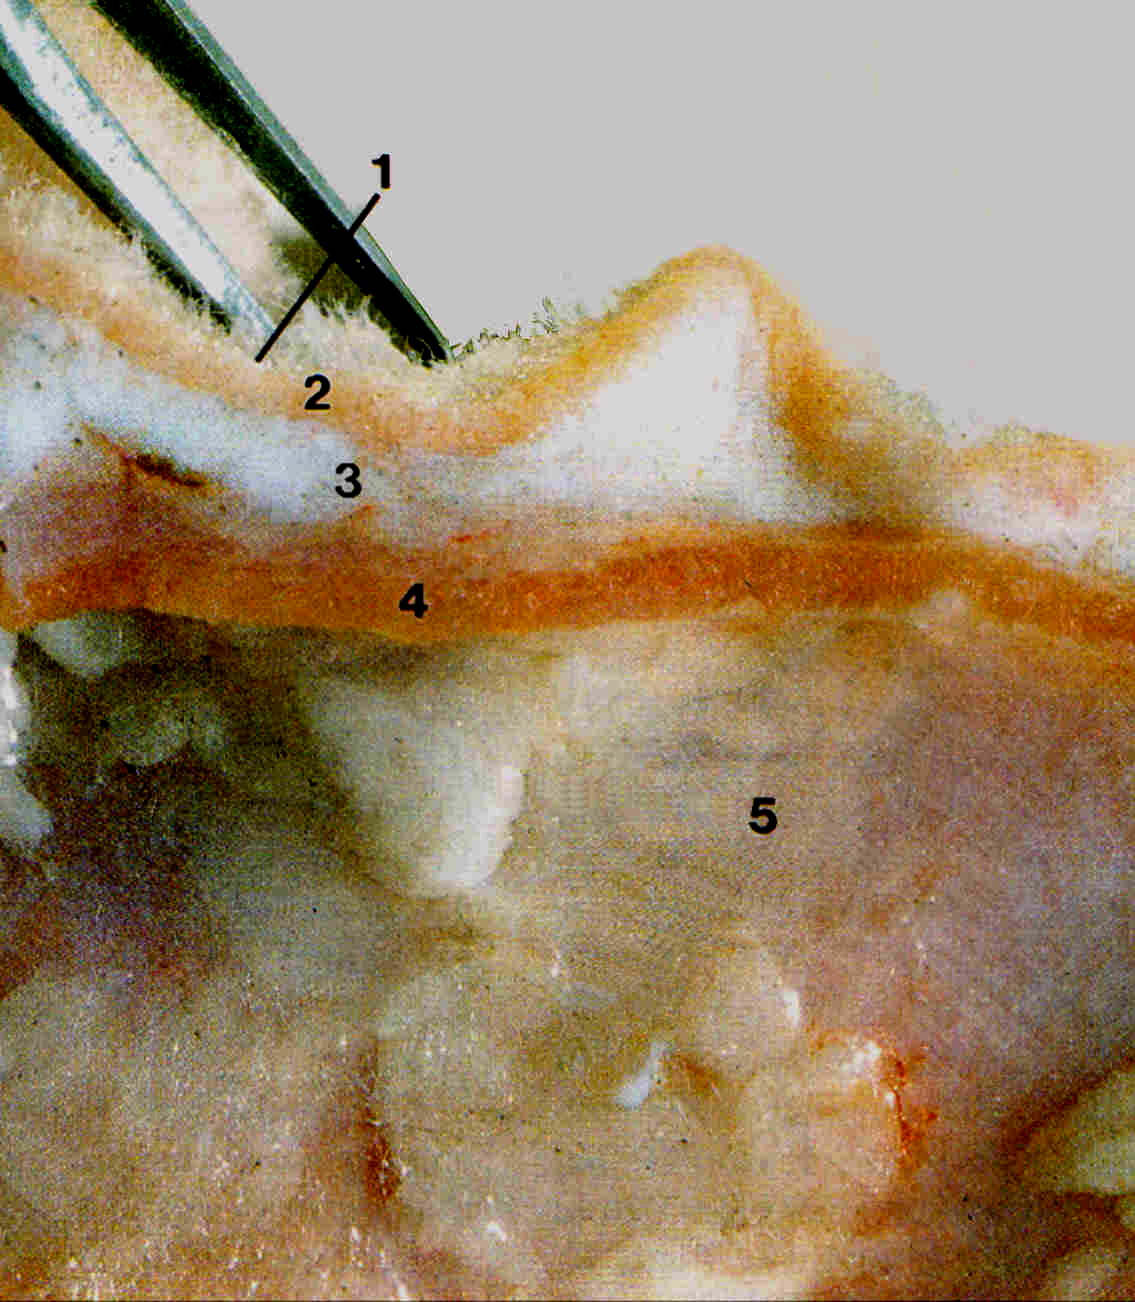
\includegraphics[width=0.7\textwidth]{mitchell.png}
  \caption{Merino sheep skin showing tissue layers. 1. epidermis with wool fibres; 2. papillary layer of dermis; 3. reticular layer of dermis; 4. areolar tissue and muscle; and 5. adipose tissue. One wrinkle is present on the right-hand side of the forceps. Forceps opening is $5 mm$. Modified from \citep{mitchell-1984}.}
  \label{fig:mitchell}
\end{figure}

%\end{document}


Only the first 2 layers curve upward in a folded section of skin, layer 3 expands to fill space under the wrinkle, layers 4 and 5 remain straight. This may be seen in Figure ~\ref{fig:mitchell}. Mitchell et al. noted that Layer2 is more elastic than Layer 3.  It appears as if wrinkles are formed either by an overgrowth of Layers 1-2, or by a shrinkage or tightening of Layer 4. Mitchell has demonstrated  that if Layer4 (and Layer 5) are dissected away from a skin specimen with wrinkles, the folds in Layers 1-2 flatten.  Therefore in a wrinkled sheep, Layer 4 is holding the skin under some tension, which relaxes when Layer 4 is removed.

Wrinkle development has been even less studied. Merino lambs are born with visible wrinkles.  \citep{bogolyubsky-1940} asserted that wrinkles were observed forming in foetal skin of Karakul and Merino lambs at around 100 days of gestation, which is about the time at which secondary derived follicles initiate \citep{fraser-1960}. A photograph of skin surface of a 10-day old Merino lamb \citep[see]{carter-1943} shows fine wrinkles of the type Carter termed {\em pin wrinkles}. Whilst studies of follicle development are extensive \citep[see]{fraser-1960,ryder-1968,maddocks-1988}, similar studies of foetal wrinkle development are lacking. 

 To bring new information to bear on wrinkle formation, this study focusses on amount, type, and arrangement of collagen in skin. Collagen is found in the dermis (layers 2 and 3) of foetal skin at the time follicles develop \citep{knight-1993}. 
\citeauthor{knight-1993} distinguish two collagen types (Type I or 'hard' collagen and Type III or 'soft' collagen) and note  that Type III is most prevalent at 75 days of gestation, and its proportion falls progressively as the foetus develops. Type I is least prevalent at day 75 and its proportion rises to over 50 percent by birth.


 In histological examination of skin, Type I or hard collagen forms thick bundles of eosin staining fibres. Its function is to bind tissues together in a rigid manner. Type III or soft or reticular collagen forms thin separate eosin staining fibres which cross-link to form a fine flexible mesh network supporting soft tissues. The strength, elasticity and flexibility of skin comes from presence of collagen and elastin fibres, and presumably variations in these properties derive from variations in amounts and proportions of these types of collagen. The basis of this study is an hypothesis that amount and type of collagen in the lower dermis determines how well the upper dermis and sub-dermis are bound together, and hence the likelihood that skin will form wrinkles.

 Collagen fibres are formed by fibroblast cells.  At 75-80 days fibroblasts appear as round, immature cells \citep{knight-1993} surrounded by reticular collagen fibres which are composed of Type III collagen and form a net-like structure. By birth fibroblasts have matured  and collagen fibres can be inter-meshed to various degrees forming thick bundles of fibres which are birefringent. If the fine reticular  or net-like fibre pattern remains, the mature sheep has soft or Type III collagen; if fibres inter-mesh and form thicker and longer bundles the mature sheep has  hard or Type I collagen. 

Collagen development, secondary follicle development and wrinkle formation  all seem to commence at the same time of 75-100 days of foetal age.  Follicle initiation ceases at birth ( 150 days) but development of collagen and wrinkles continues into maturity. In this study we look at end point of development - that is we study collagen and follicles in adult sheep with and without wrinkles. 


\section{Materials and Methods}
\label{sec:matmeth}
The experimental design was to choose, by visual inspection, individual sheep with wrinkle-free skin and wrinkly skin from each of several Australian Merino flocks. 

Two trials were conducted
\begin{description}
\item[Trial 1]  Two sheep were chosen from each of six SRS\textsuperscript{\tiny\textregistered} Merino stud flocks, one wrinkle-free and one wrinkled. This is a randomised block design without replication .  The blocks are the flocks, and the treatment is presence or absence of wrinkle.
\item[Trial 2]  Eighteen sheep were chosen from each of two commercial flocks, nine wrinkle-free and nine with wrinkles. This is a randomised block design with replication. The second of these two flocks was more wrinkled. 
\end{description} 



\subsection{Skin samples}
In Trial 1 a biopsy sample was taken from the mid-side position on each sheep and specimens were trimmed \citep{maddocks-1988} before processing, so that only Layers 1-3  were present for histological observation.


In Trial 2 , for the sheep with wrinkled skins, skin biopsies were collected from on-wrinkle as well as off-wrinkle positions. For the wrinkle-free sheep only one biopsy sample was collected. These specimens were not trimmed, so they included Layers 1-3,  and in some cases part of Layers 4 and 5, depending on the depth of biopsy.

Mid-side skin biopsy samples were collected using a 10-millimetre
circular trephine (Acu Punch® skin biopsy punches, Acuderm, Inc.) and
fixed in 10\% buffered formol saline solution. 

\subsection{Histological skin processing and observations}
\subsubsection{Collagen observations}

Skin samples used for haematoxylin and eosin (H-E) and picrosirius red (PSR) staining, were fixed in 10\% neutral buffered formalin for 24 hours before being processed to wax in an automated tissue processing platform (Shandon Excelsior, Thermo Scientific, USA), and then embedded in paraffin wax. Four micron sections were cut and placed onto slides for H-E staining for tissue morphology. Serial section was also employed on a separate slide for PSR staining to highlight
collagen content. Staining was done manually.

Sections were then reviewed microscopically (BX53 Olympus, Australia)), and images taken on 3 CCD camera (DP72, Olympus, Australia) under both bright field and polarised conditions.

For PSR collagen analysis, a 40x objective was employed at a fixed exposure to take high power images of 5 random lower dermal fields of view for image analysis aimed at determining amount of collagen in each field. 

The five images for each sample were then uploaded for quantitative analysis via the ImagePro Plus (Media Cybernetics, USA) 7.1 software in which thresholds were set to count all pixels comprising of the red staining fibres in the PSR stained specimen field.  This provided a measure of area of the field occupied by red stained collagen fibres.

A measure of total amount of collagen in the field could be obtained by allowing for the intensity of red staining of each pixel. This  is a measure density of collagen within the pixel and depth of collagen through the thickness of the section.  Grey-values for each pixel were converted to optical density, and optical densities summed (ie integrated) over all pixels in the field.
Means were calculated for each specimen, averaged over 5 fields, and graphed.  Optical density data for each field subjected to analysis of variance to test for differences between wrinkle-free and wrinkled sheep, and , in Trial 2, to test for differences between on-wrinkle and off-wrinkle specimens within wrinkled sheep.
All specimens were measured in this way, and this is the main quantitative result of the study.

Polarised light was employed to determine type of collagen present within each sample. Bundles of fibrils stained with Sirius Red dye are strongly birefringent; single fibrils as in reticular collagen are not \citep{cuttle-2005}.
Collagen stained with PSR has enhanced birefringence compared with that in H-E stained sections \citep{junqueira-1979}. Under polarised light sections show coloured red,orange, yellow, or green, in order of thickness of bundles of fibres. Thus red or orange should indicate Type I or hard collagen (which has thick bundles of fibres) while yellow or green should indicate Type III collagen which has individual fibres in a net-like structure.

Attempts to use polarised light images to make quantitative assessments of amounts of each Type of collagen have been criticised \citep{lattouf-2014}.  The main issue seems to be that birefringence is directional, only fibres aligned with the direction of polarisation will show colours. We refrained from attempting this quantification, so our polarised light results are only qualitative.


\subsection{Statistical Methods}

Data were imported into the R statistical program \citep{rcoreteam-2017} and analysed using the {\em aov()} function for analysis of variance.
Allowance was made for sub-sampling design by choosing  an appropriate error level for F tests in analysis of variance. 

\section{Results}
We look first at overall morphology of skin specimens, then at details of collagen structure, and finally at related observations

\subsection{Skin tissue Morphology}
Pairs of wrinkle-free and wrinkled sheep from each flock in Trials 1 and 2 showed consistent visual differences in their tissue structure. Figure~\ref{fig:trial24xhe} shows vertical sections stained with H-E from a wrinkled and wrinkle-free pair of sheep. 

%\documentclass{article}
%\usepackage{graphicx,subfigure}
%\usepackage{caption,rotating}
%\begin{document}

\begin{figure}[!h]
\centering
\captionsetup{width=0.7\textwidth}
 \subfigure[Sheep 3437 Wrinkled]{
%   \label{fig:trial1he(i)}
%   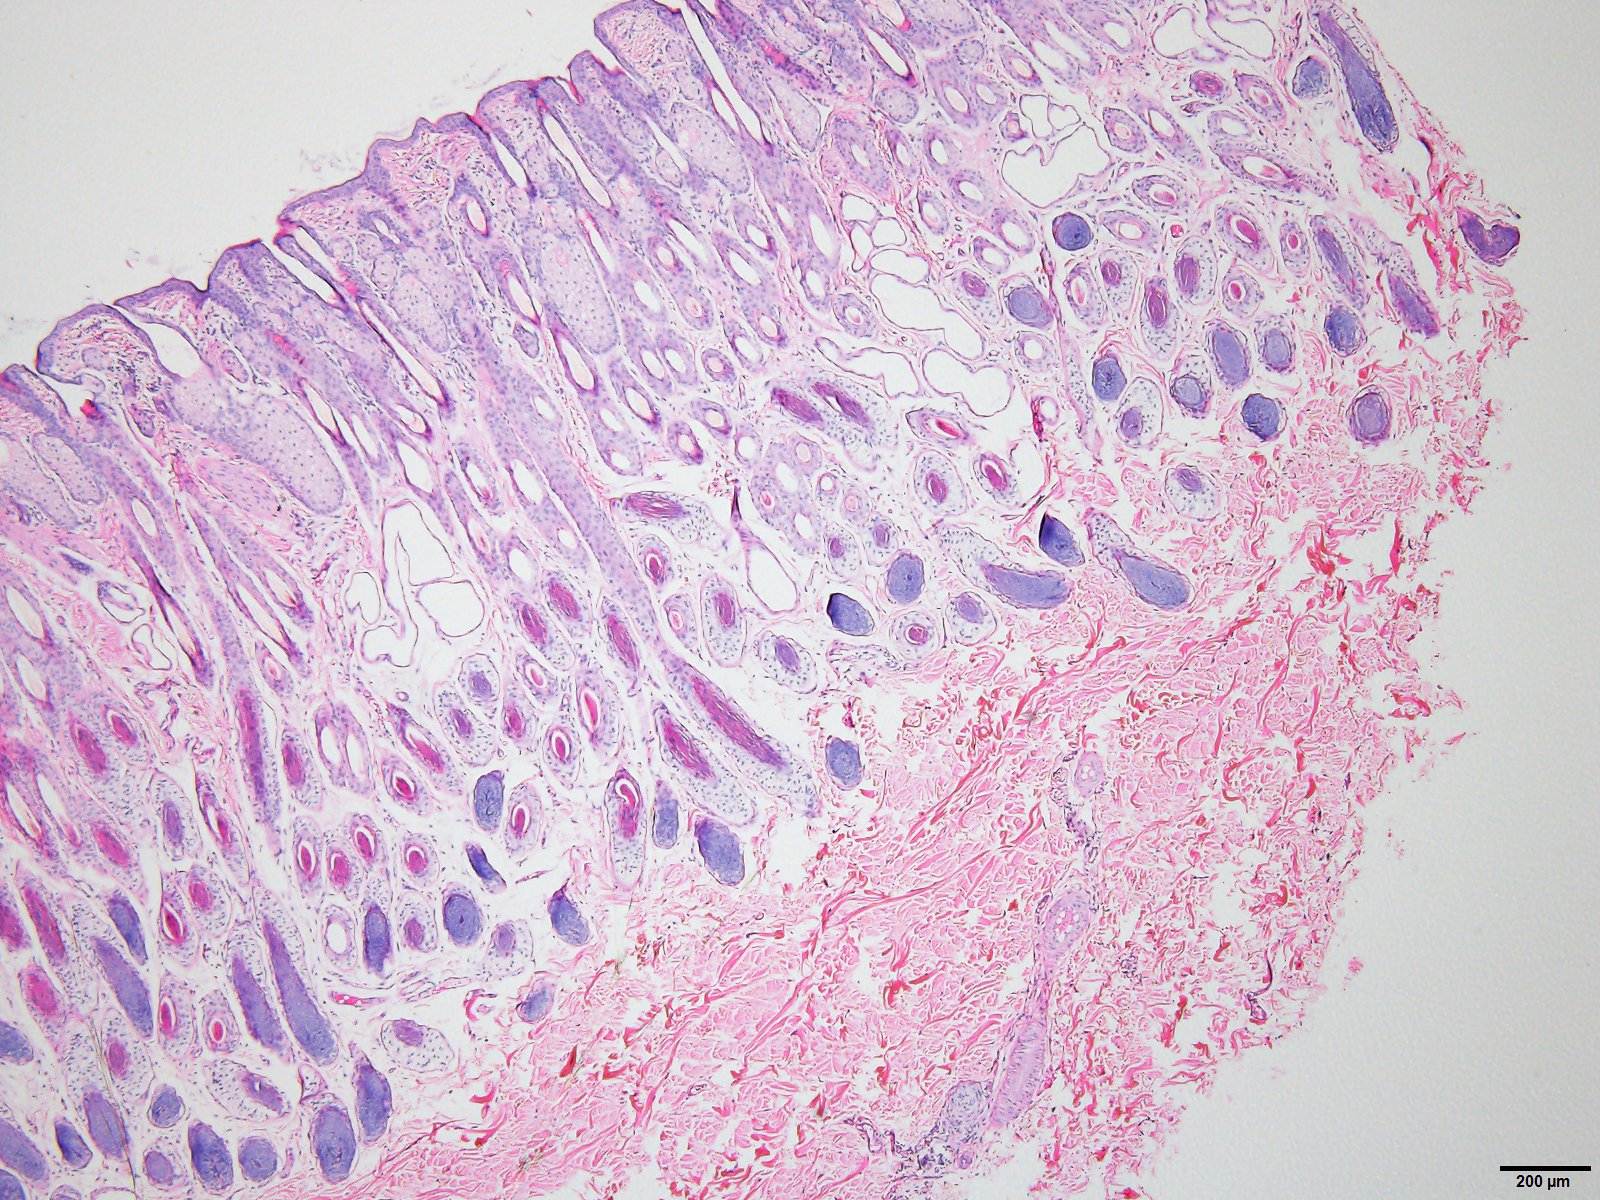
\includegraphics[scale=0.20]{3437_on_wrinkle_4x.jpg}
%    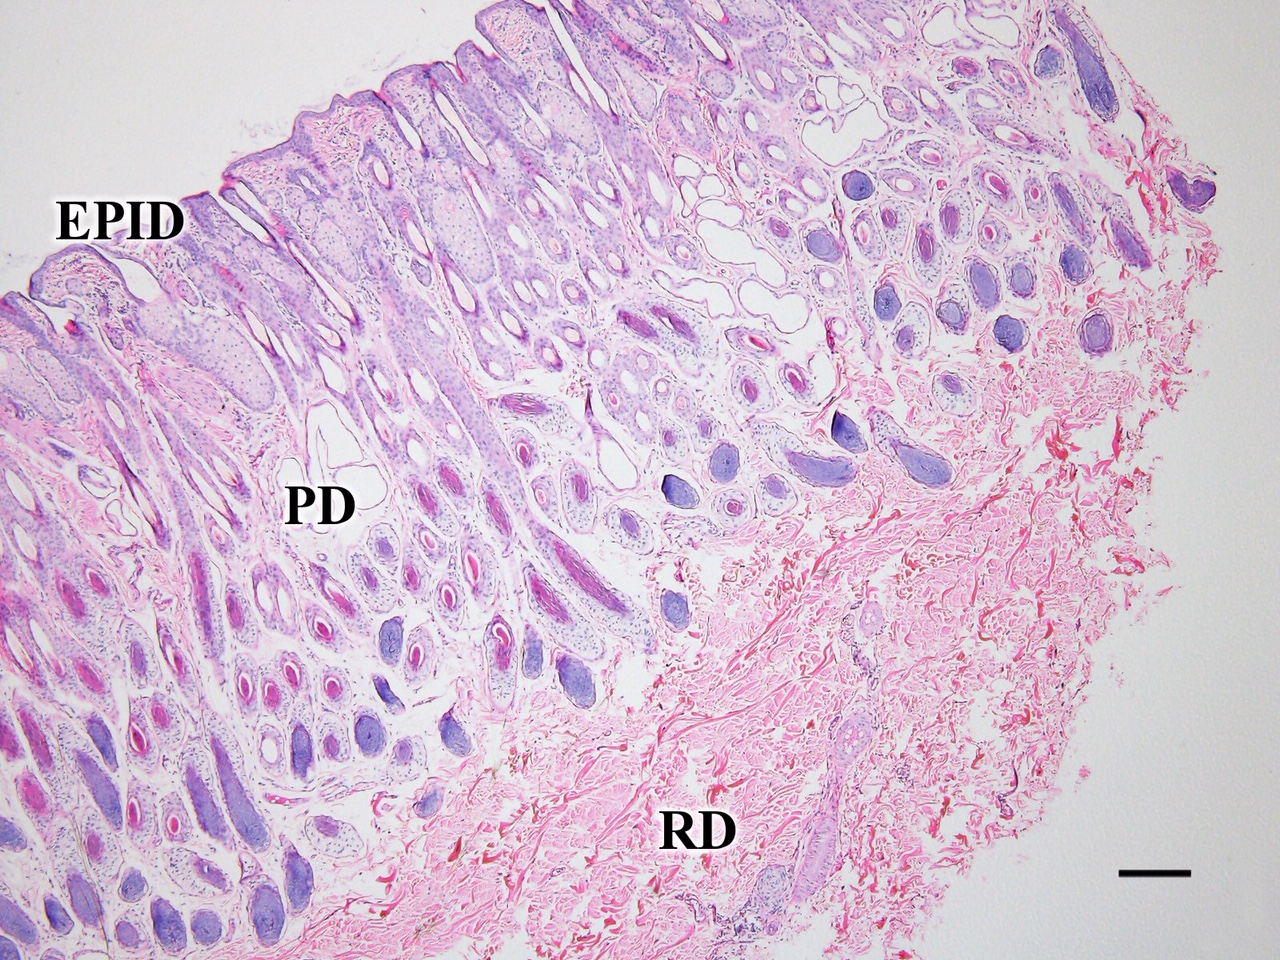
\includegraphics[scale=0.10]{fig2a.jpg}
     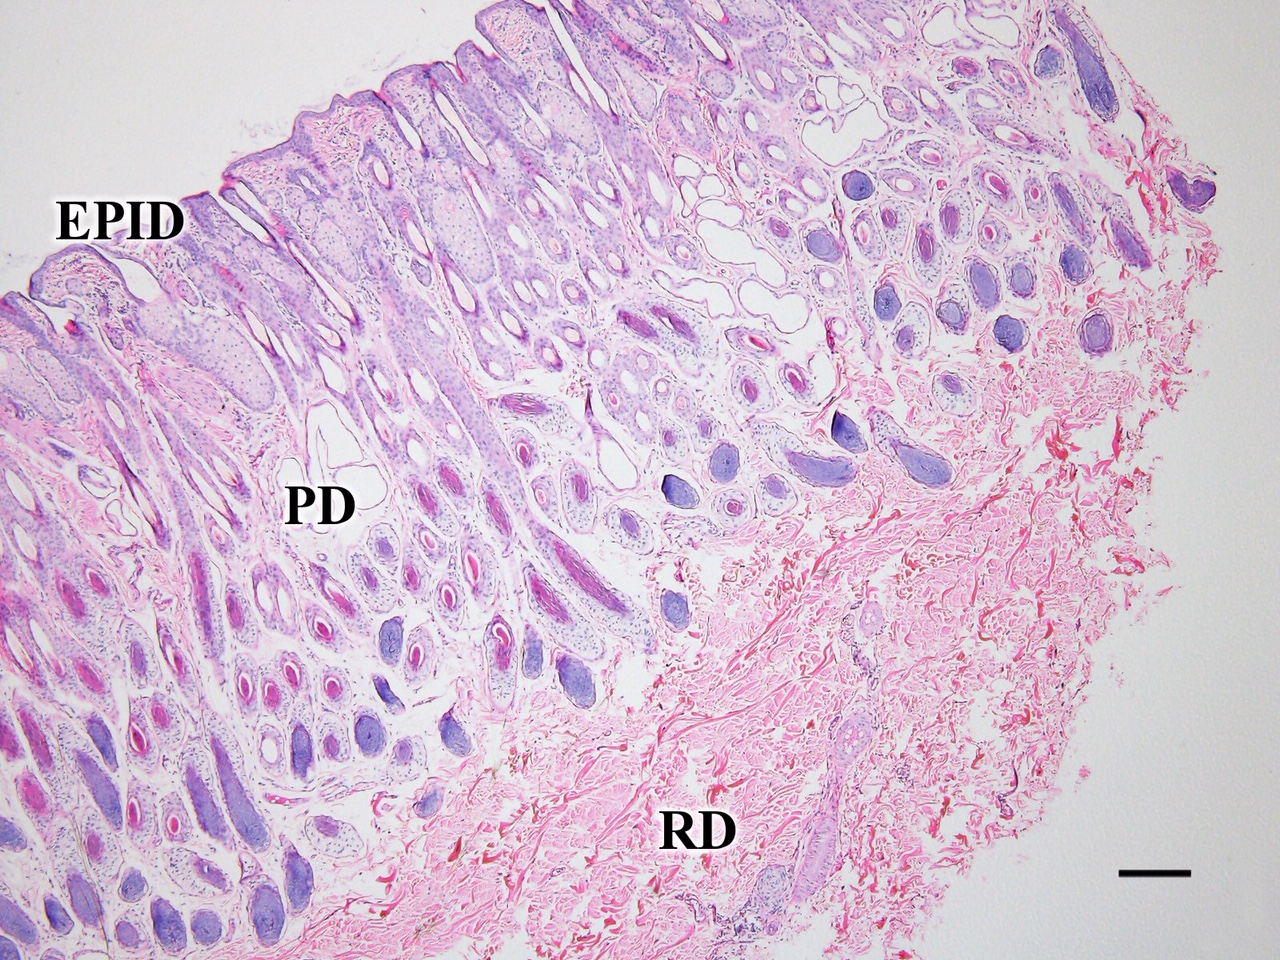
\includegraphics[width=0.7\textwidth]{fig2a.jpg}
% 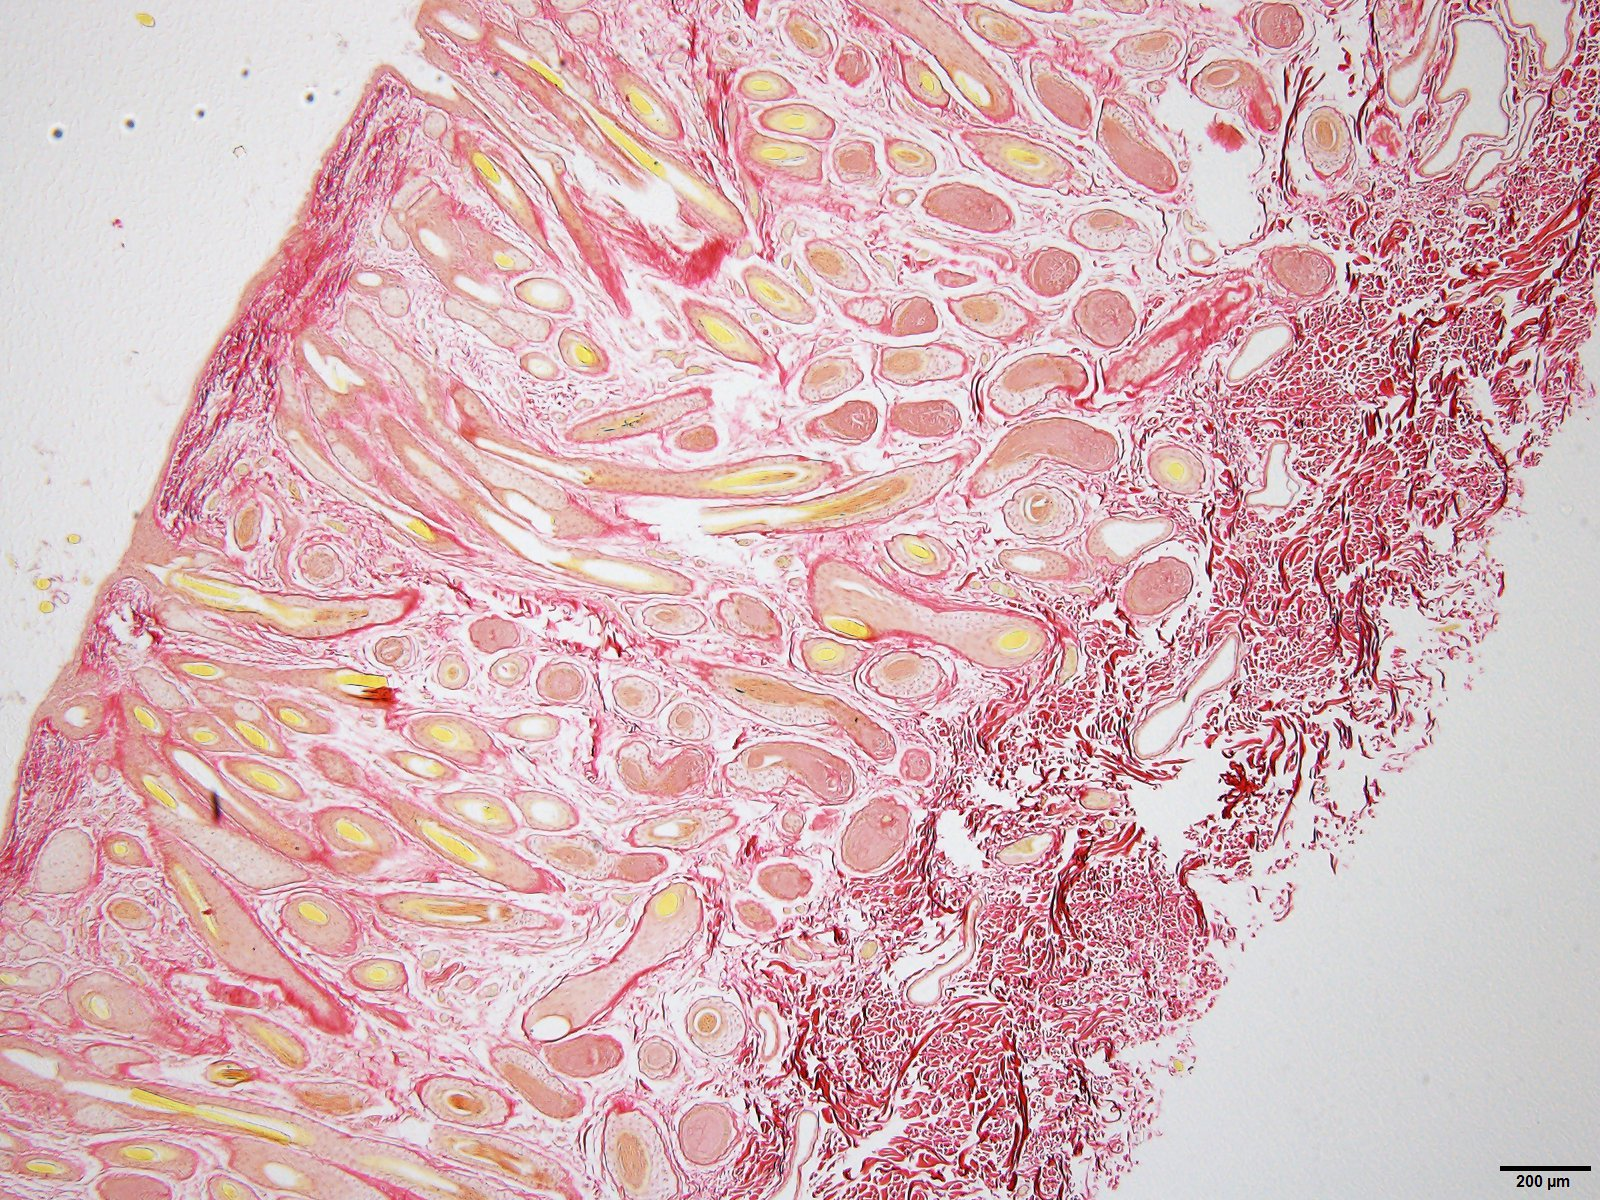
\includegraphics[width=1.0\textwidth]{w479-2-rigid.jpg}
  }
 \subfigure[Sheep 3457 Wrinkle-free]{
%   \label{fig:trial1he(ii)}
%   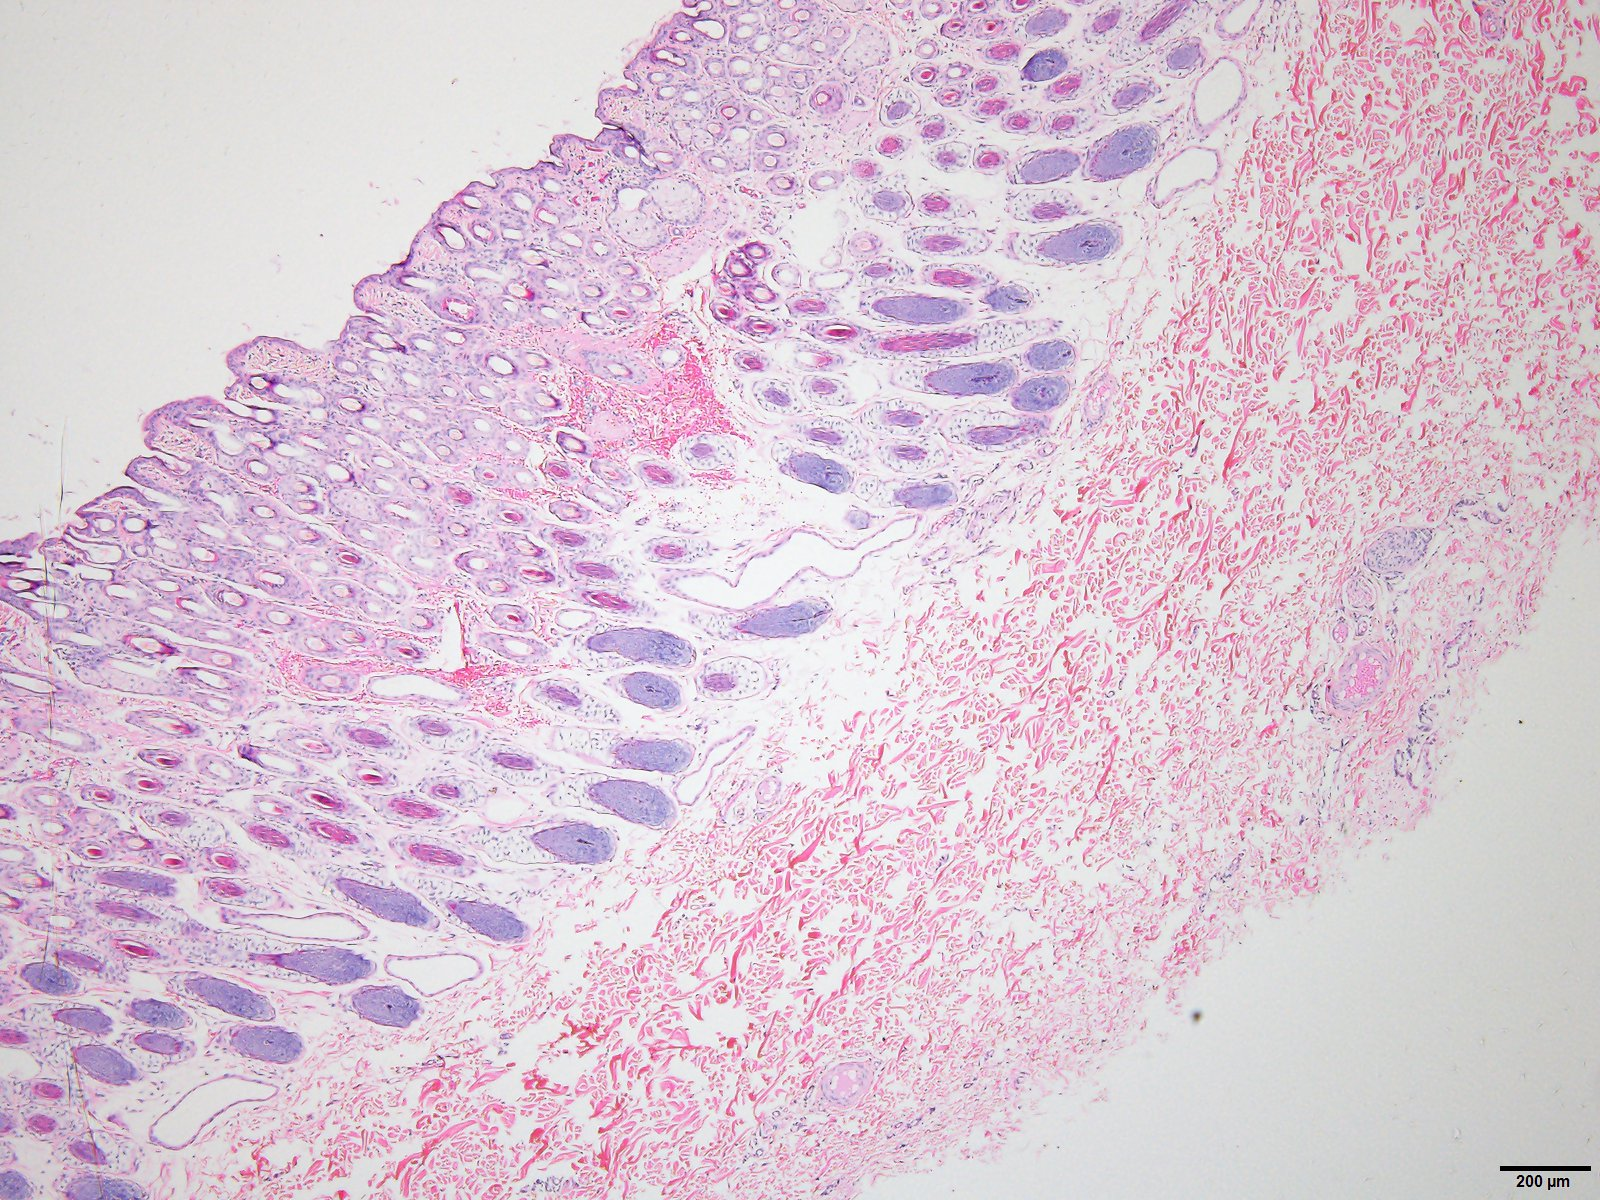
\includegraphics[scale=0.20]{JW_3457_smooth_4x.jpg}
%    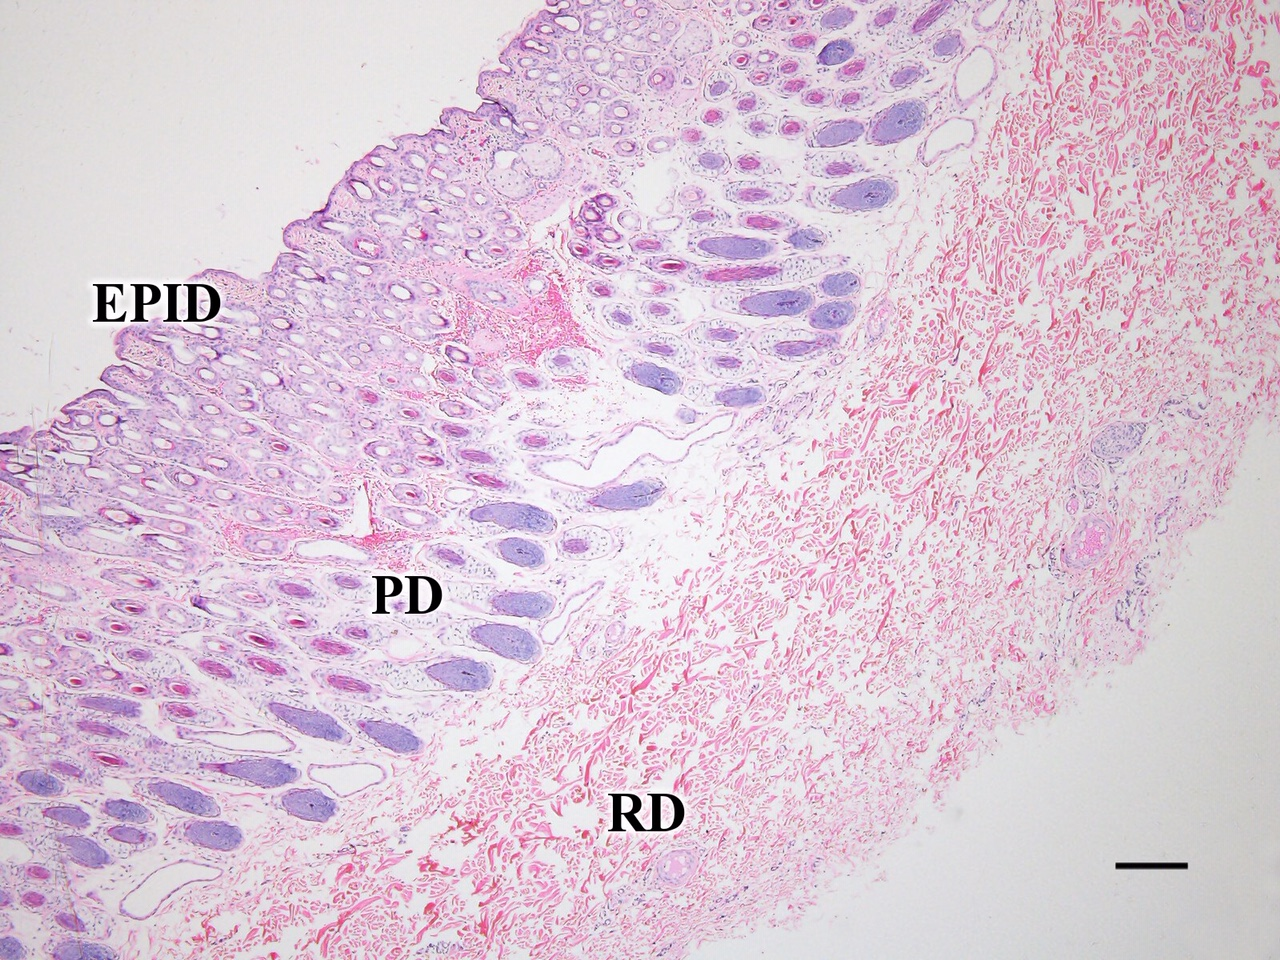
\includegraphics[scale=0.10]{fig2b.jpg}
     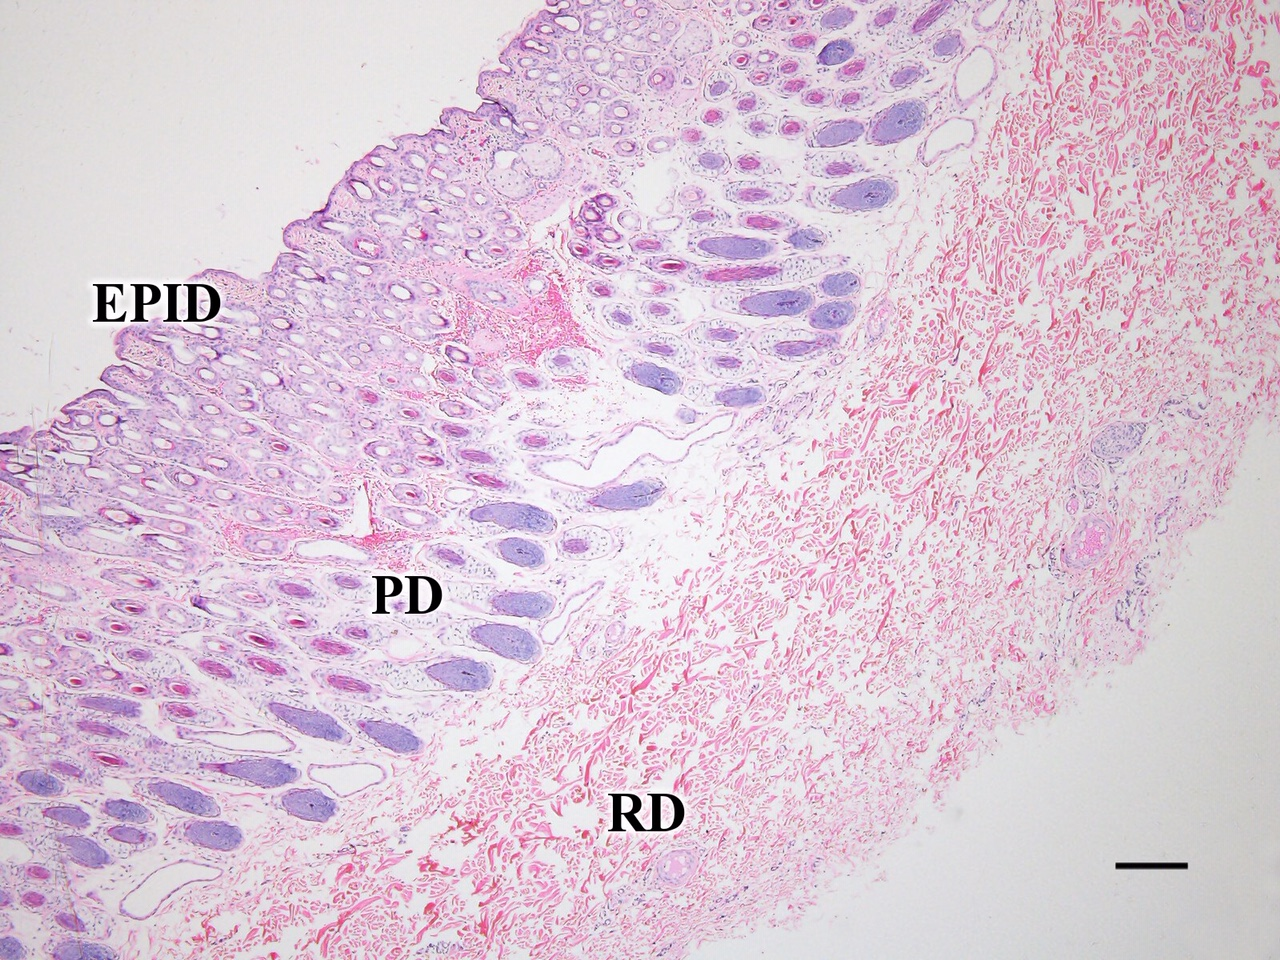
\includegraphics[width=0.7\textwidth]{fig2b.jpg}
  }
  \caption{Vertical sections from a wrinkled (a) and a wrinkle-free (b)  sheep from Trial 2 flock 1 stained with H-E. Skin layers are: {\bf EPID} epidermis, {\bf PD} papillary dermis, and {\bf RD} reticular dermis. Scale bar is 200 $\mu m$ }
\vfill
  \label{fig:trial24xhe}
\end{figure}

%\end{document}



The connective tissue of the lower dermis below follicle bulbs was more heavily stained in wrinkled sheep. The stained lower dermal material is in clumps in wrinkled sheep, whereas in wrinkle-free sheep the proximal connective tissue has a finer more uniform structure. 
These differences were consistent across all sheep.

Although the Trial 2 biopsy samples were not trimmed before sectioning, the specimens displayed in Figure~\ref{fig:trial24xhe} do not show any layers below Layer 3.  This is because biopsy specimens are not regularly taken deep enough to include layers 4 and 5.

 To check if connective tissue extends into Layers 4 and 5  we look at a deeper biopsy specimen that has Layer 4 intact.   Figure~\ref{fig:trial2he} shows one example section which is from a wrinkled sheep.
%\documentclass{article}
%\usepackage{graphicx,subfigure}
%\begin{document}

\begin{figure}[!h]
  \centering
  \captionsetup{width=0.7\textwidth}
%  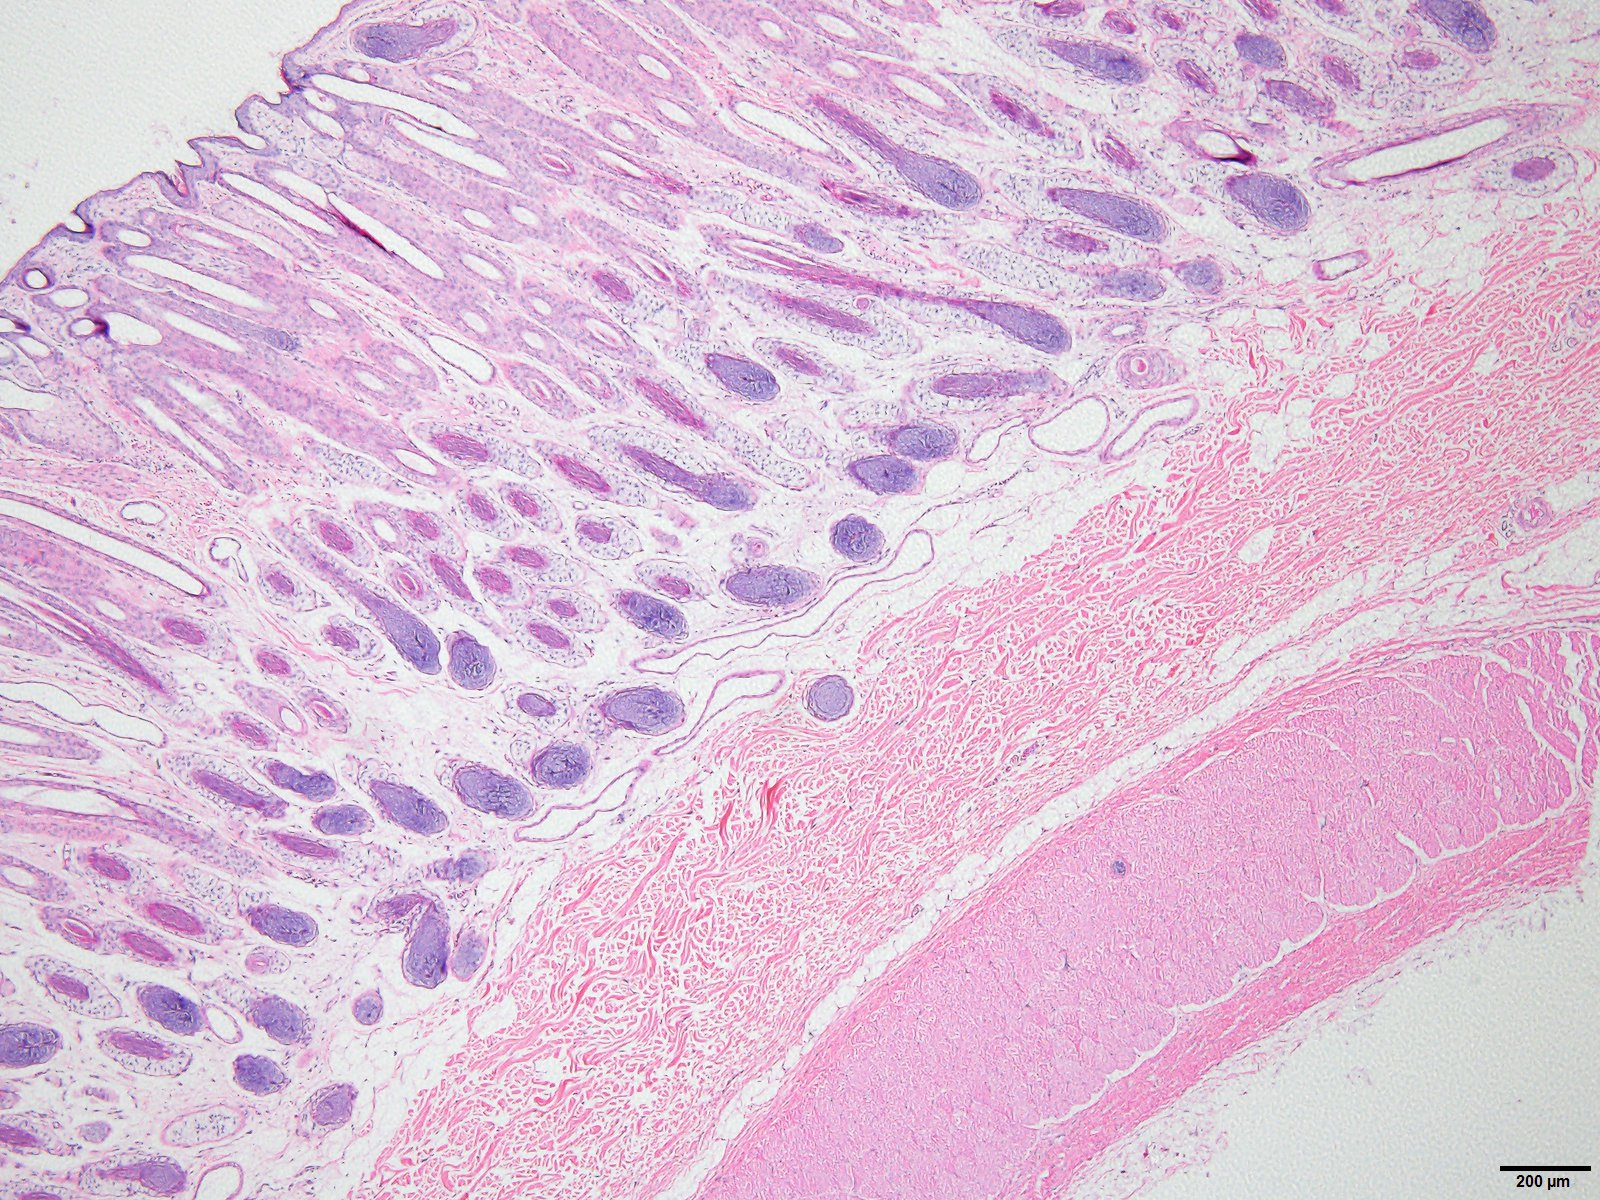
\includegraphics[width=1.0\textwidth]{3456_4layers_4x.jpg}
  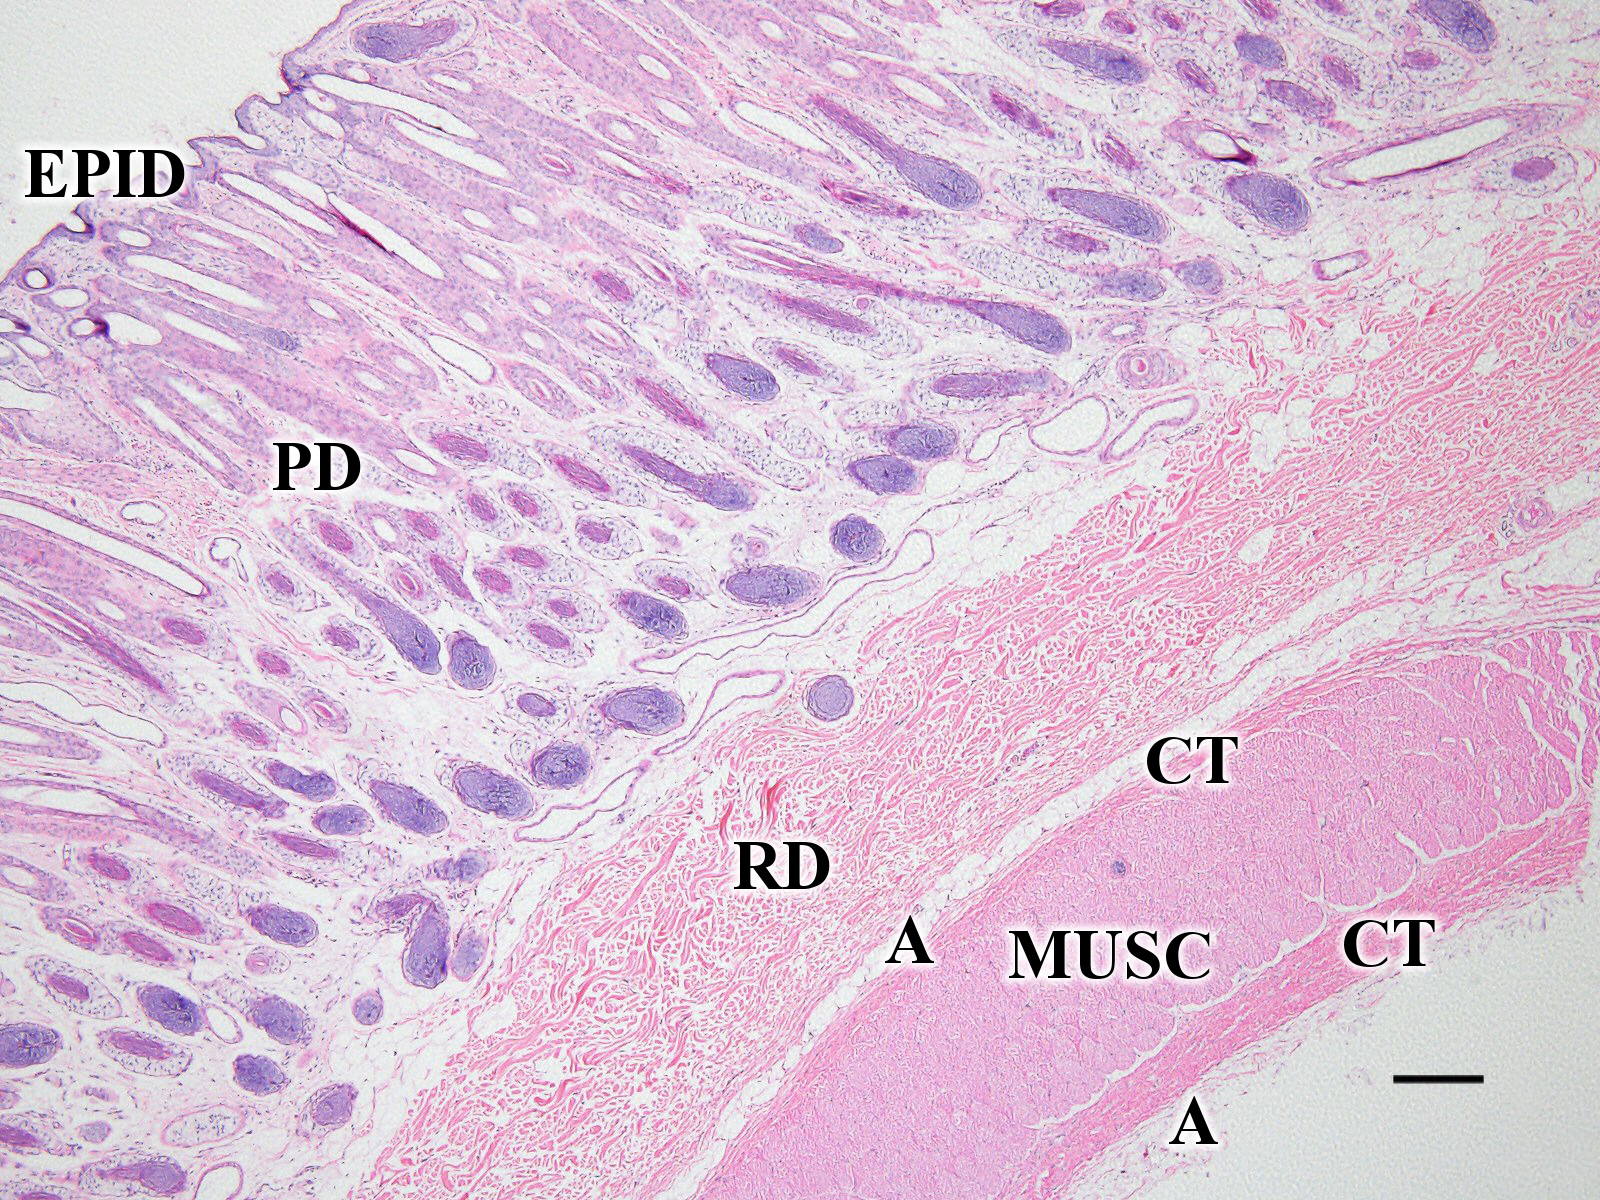
\includegraphics[width=0.7\textwidth]{fig3.jpg}
% 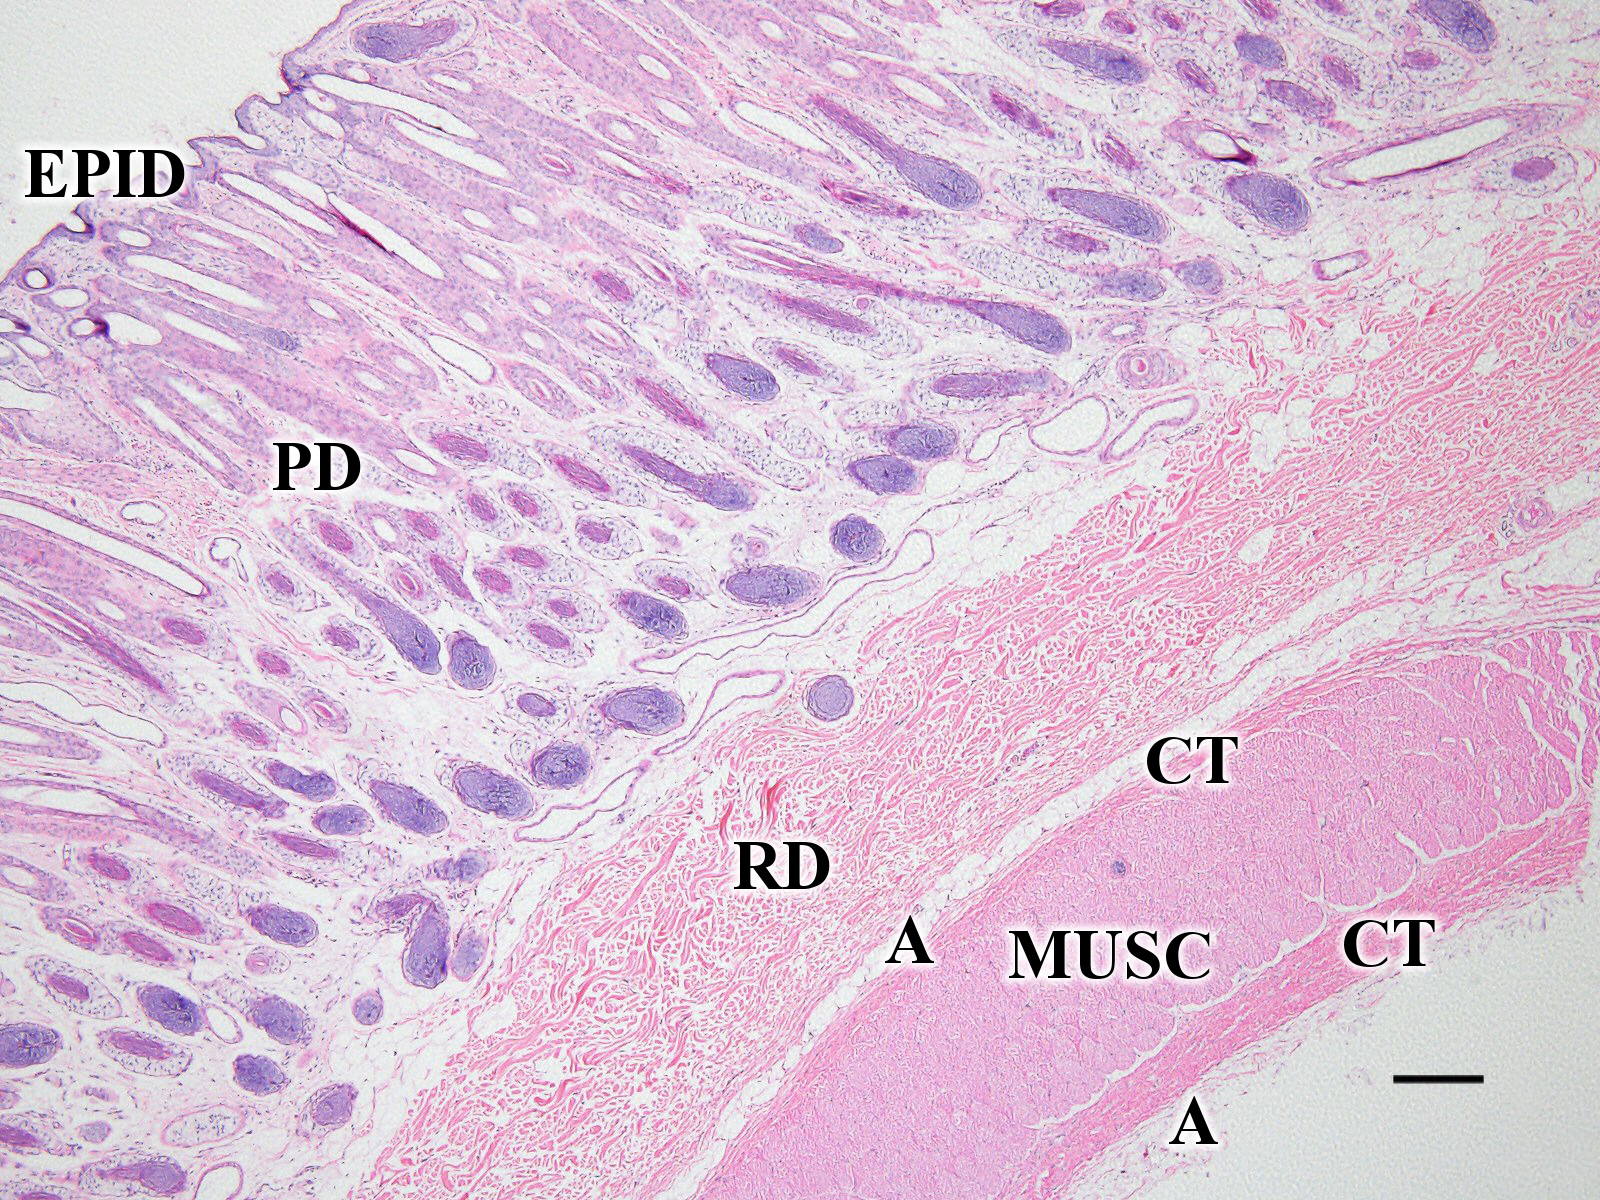
\includegraphics[scale=0.10]{fig3.jpg}
  \caption{Vertical section from a wrinkled sheep (3456) from Trial 2 Flock 1 stained with H-E. This section is from an untrimmed biopsy specimen and shows all 5 layers  identified by Mitchell: {\bf EPID} epidermis, {\bf PD} papillary dermis, {\bf RD} reticular dermis, {\bf MUSC} muscle, and {\bf A} adipose tissue). In addition there are two layers of {\bf CT} connective tissue, either side of the muscle layer, and a thin layer of {\bf A} adipose tissue between the reticular dermis and the muscle. Scale bar is $200\mu m$.}
  \label{fig:trial2he}
\end{figure}

%\end{document}



Figure~\ref{fig:trial2he} shows connective tissue in Layer 3 (lower or reticular dermis), followed by a thin layer of adipose tissue , then a wider layer of muscle tissue  (stained pink with eosin) evidently bordered by thin bands of connective tissue, which has a denser appearance  compared to connective tissue in the reticular dermis. A trace of adipose tissue is present below the muscle layer,as in Figure~/ref{fig:mitchell}; the biopsy specimen was not taken deep enough to include all of Layer 5.


Our focus is on connective tissue in the lower dermis. We wish to quantify and qualify the way in which it differs between wrinkled and wrinkle-free sheep.

\subsection{Detailed morphology of connective tissue} 
The stain picrosirius red (PSR) differentiates collagen from other components of connective tissue. Figure~\ref{fig:trial2psr} shows a section from the same sheep as Figure~\ref{fig:trial2he} stained with PSR and examined with bright field microscopy. 
%\documentclass{article}
%\usepackage{graphicx,subfigure}
%\begin{document}

\begin{figure}[!h]
  \centering
  \captionsetup{width=0.7\textwidth}
% 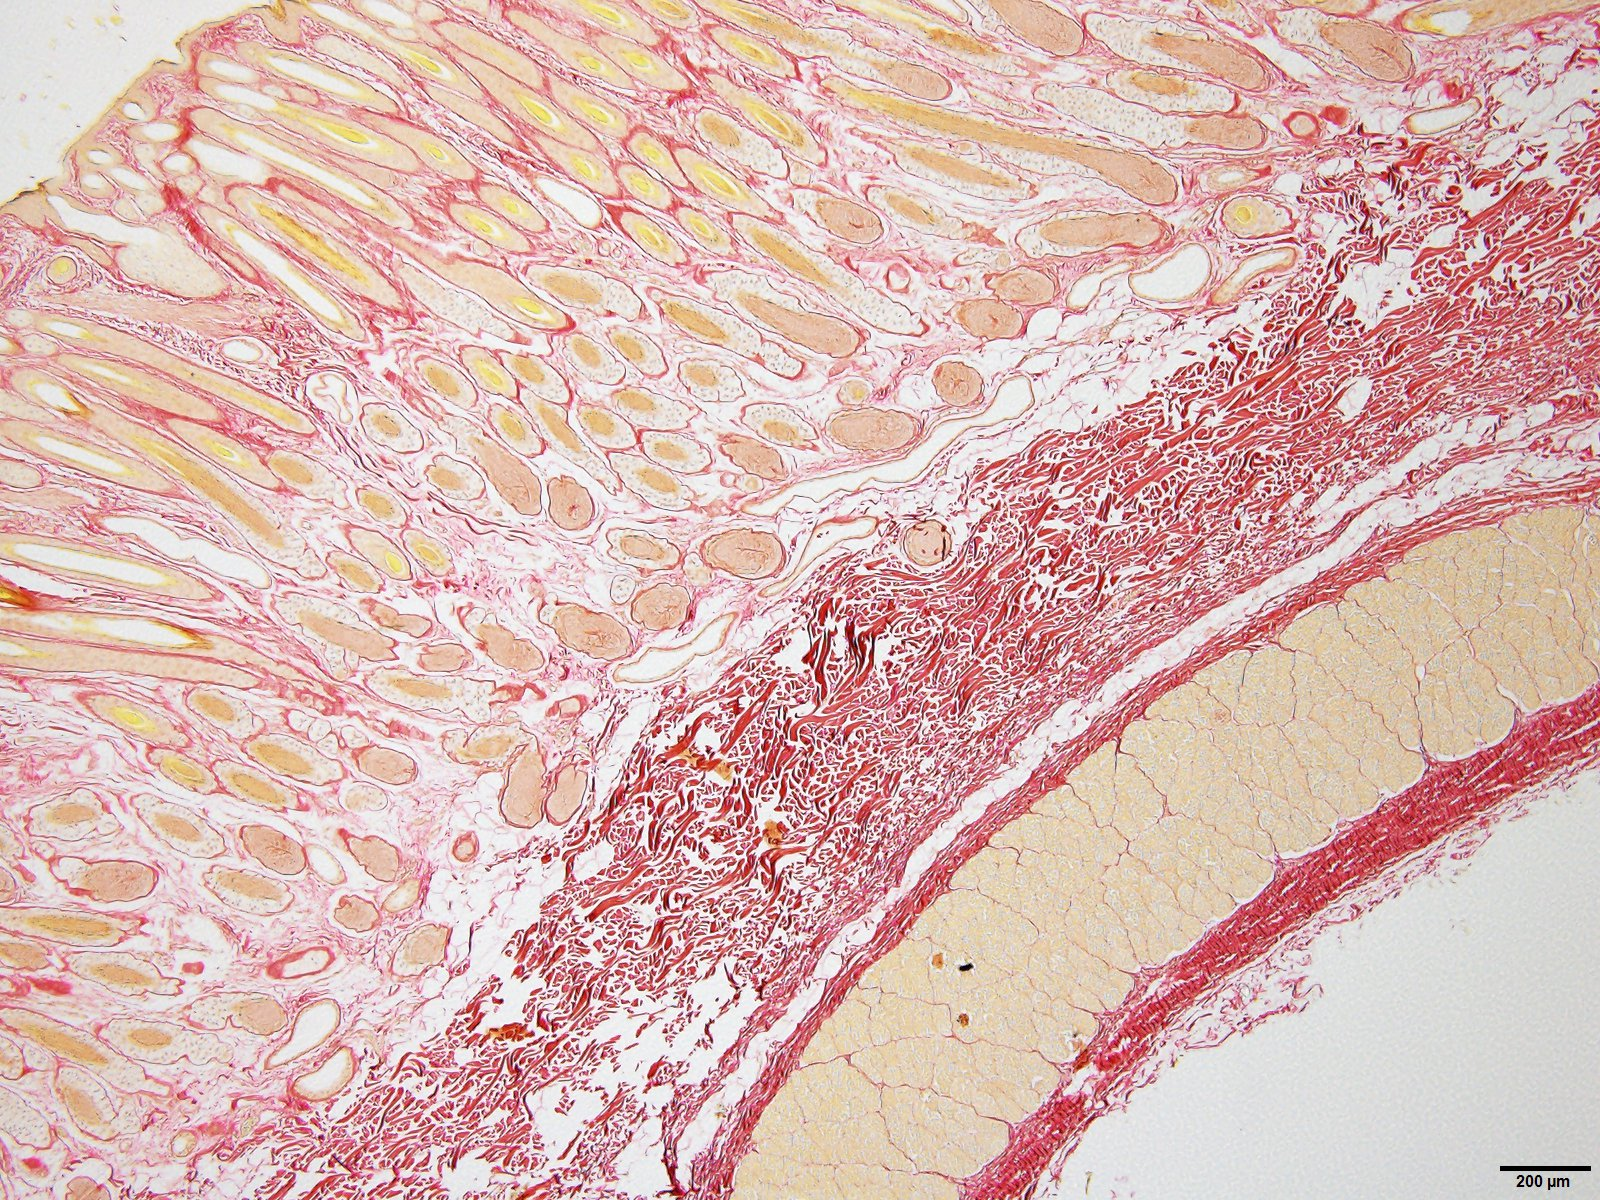
\includegraphics[width=1.0\textwidth]{3456_4layers_4x_PSR.jpg}
  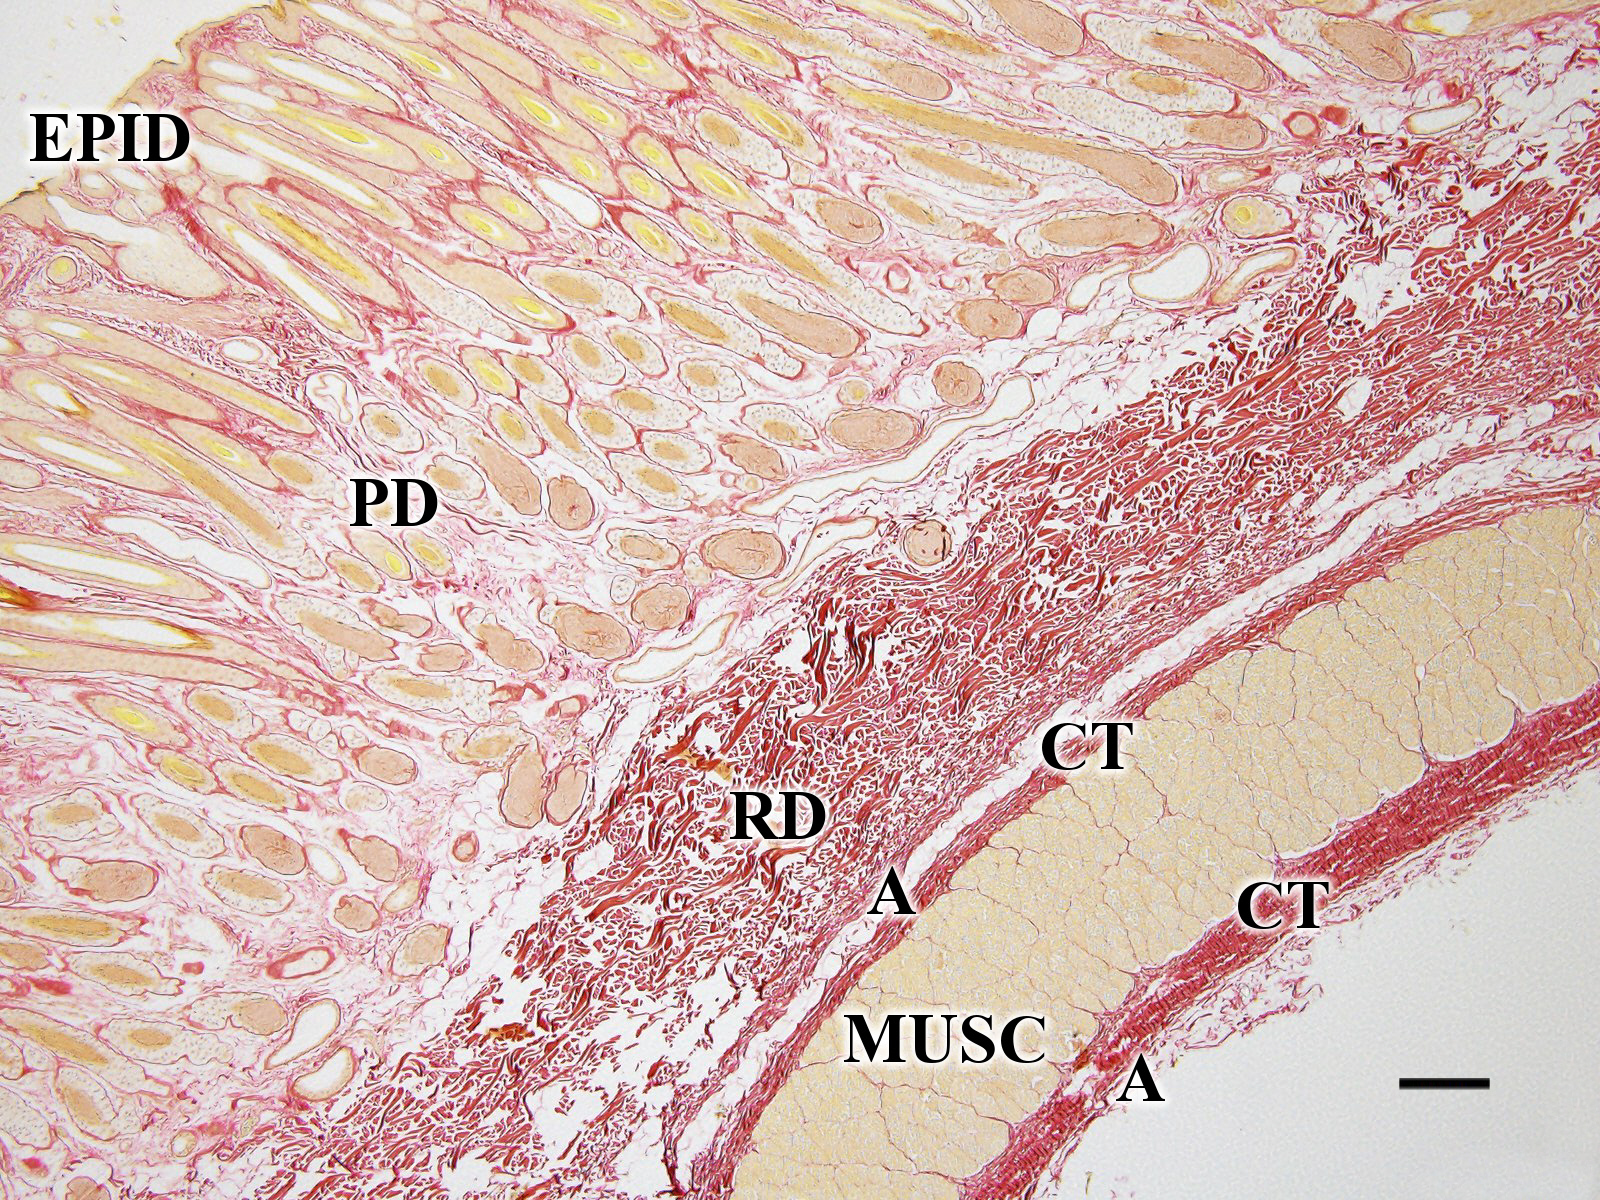
\includegraphics[width=0.7\textwidth]{fig4.jpg}
% 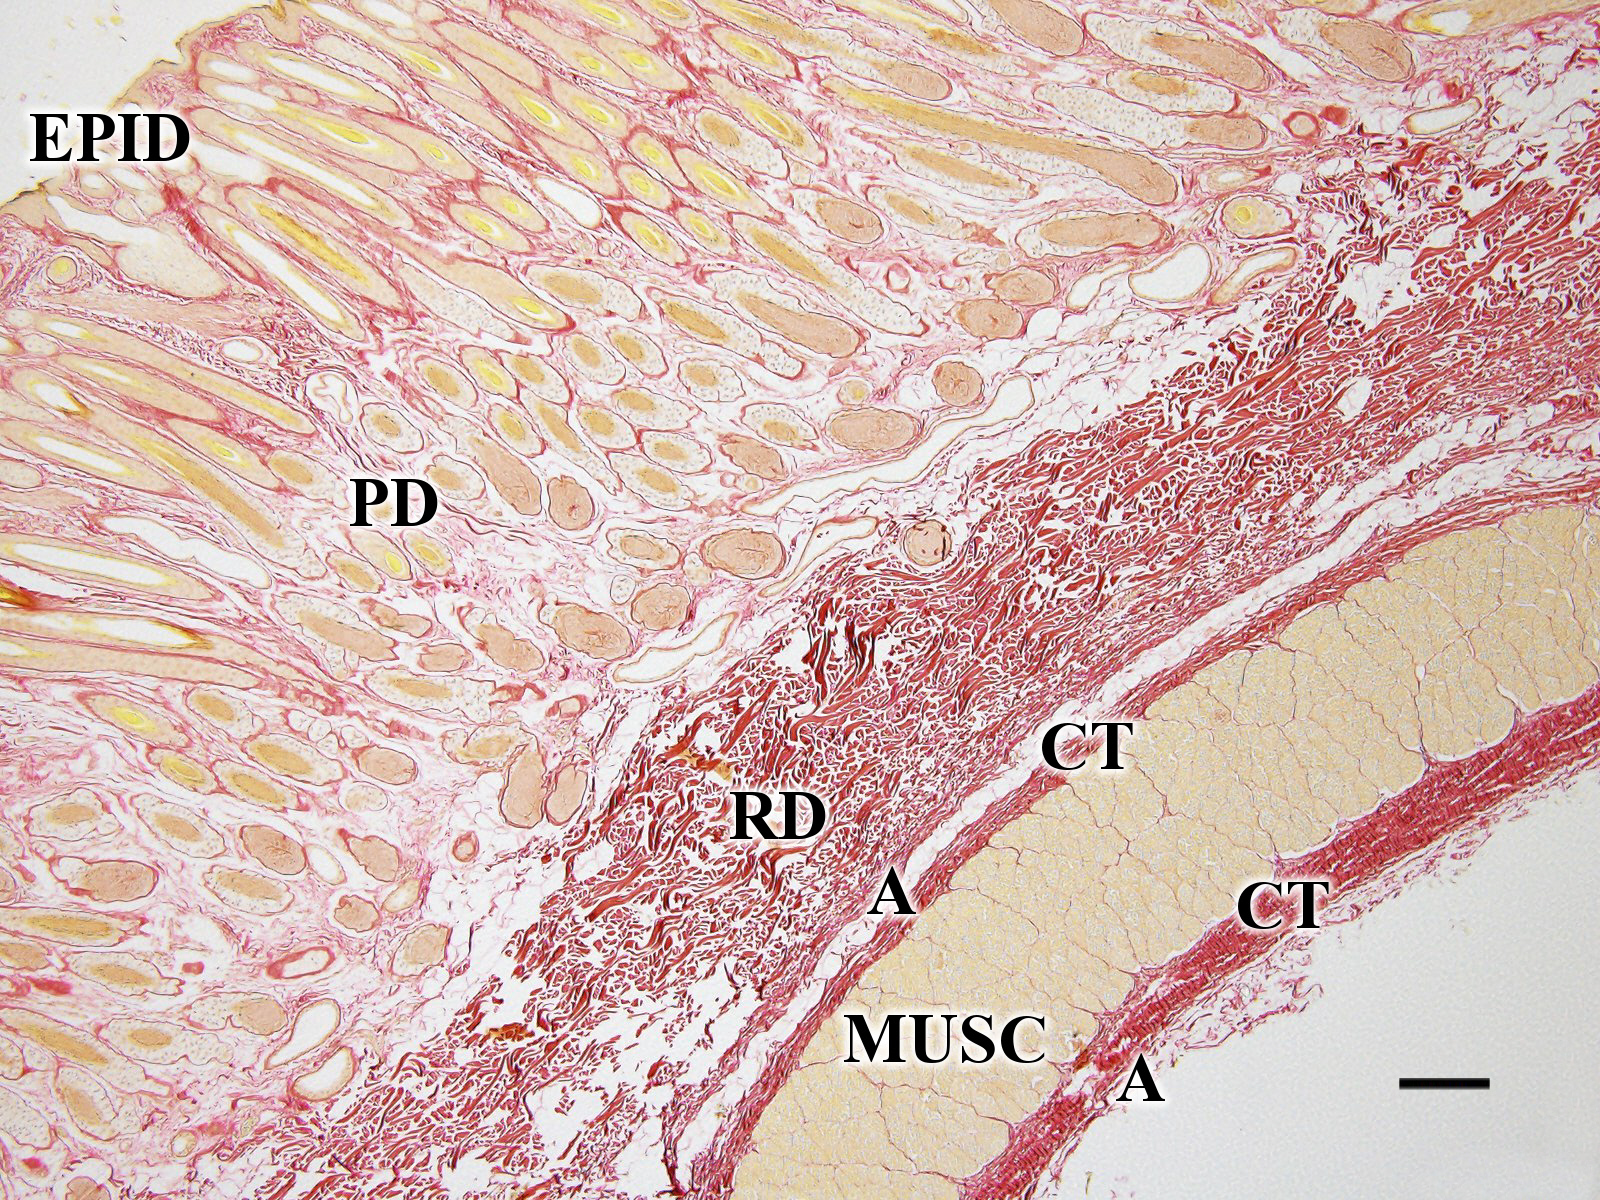
\includegraphics[scale=0.10]{fig4.jpg}
  \caption{Vertical section from a wrinkled sheep (3456) from Trial 2 Flock 1 stained with PSR and viewed with bright field microscope. This section is from an untrimmed biopsy specimen and shows all 5 layers identified by Mitchell: {\bf EPID} epidermis, {\bf PD} papillary dermis, {\bf RD} reticular dermis, {\bf MUSC} muscle, and {\bf A} adipose tissue). In addition there are two layers of {\bf CT} connective tissue, either side of the muscle layer, and a thin layer of {\bf A} adipose tissue between the reticular dermis and the muscle. Scale bar is $200\mu m$.}
  \label{fig:trial2psr}
\end{figure}

%\end{document}


Collagen is stained red. Some collagen is present in Layer 2 (papillary dermis), a dense band of collagen occurs in Layer 3 (sub-papillary dermis), and two narrow bands of very dense collagen are present either side of the muscle tissue which is stained yellow by the PSR stain.   Wool fibres and follicle bulbs are stained yellow by the picric acid component of PSR. Within the  muscle tissue are tiny tracks of red stained connective tissue.
The connective tissue in layer 4 is separated from that in Layer 3 by a thin band of adipose tissue and appears to have a different structure.  Our focus is on connective tissue in the reticular dermis, because this tissue determines how strongly the upper dermis is bound to the hypodermis.


\subsubsection{Amount of collagen}
Since the nature of the connective tissue in Layer 3 is what seems to differ between wrinkled and wrinkle-free sheep, we attempt to quantify  it.

To quantify collagen in Layer 3, five fields under a 40x objective were chosen at random from within Layer 3  of each PSR stained section from each sheep.  A typical image from one field of a wrinkled and a wrinkle-free sheep is shown in Figure~\ref{fig:psr40x}.
%\documentclass{article}
%\usepackage{graphicx,subfigure}
%\usepackage{caption,rotating}
%\begin{document}

\begin{figure}[!h]
\centering
\captionsetup{width=0.92\textwidth}
 \subfigure[Sheep 3437 Wrinkled]{
%   \label{fig:trial1he(i)}
%   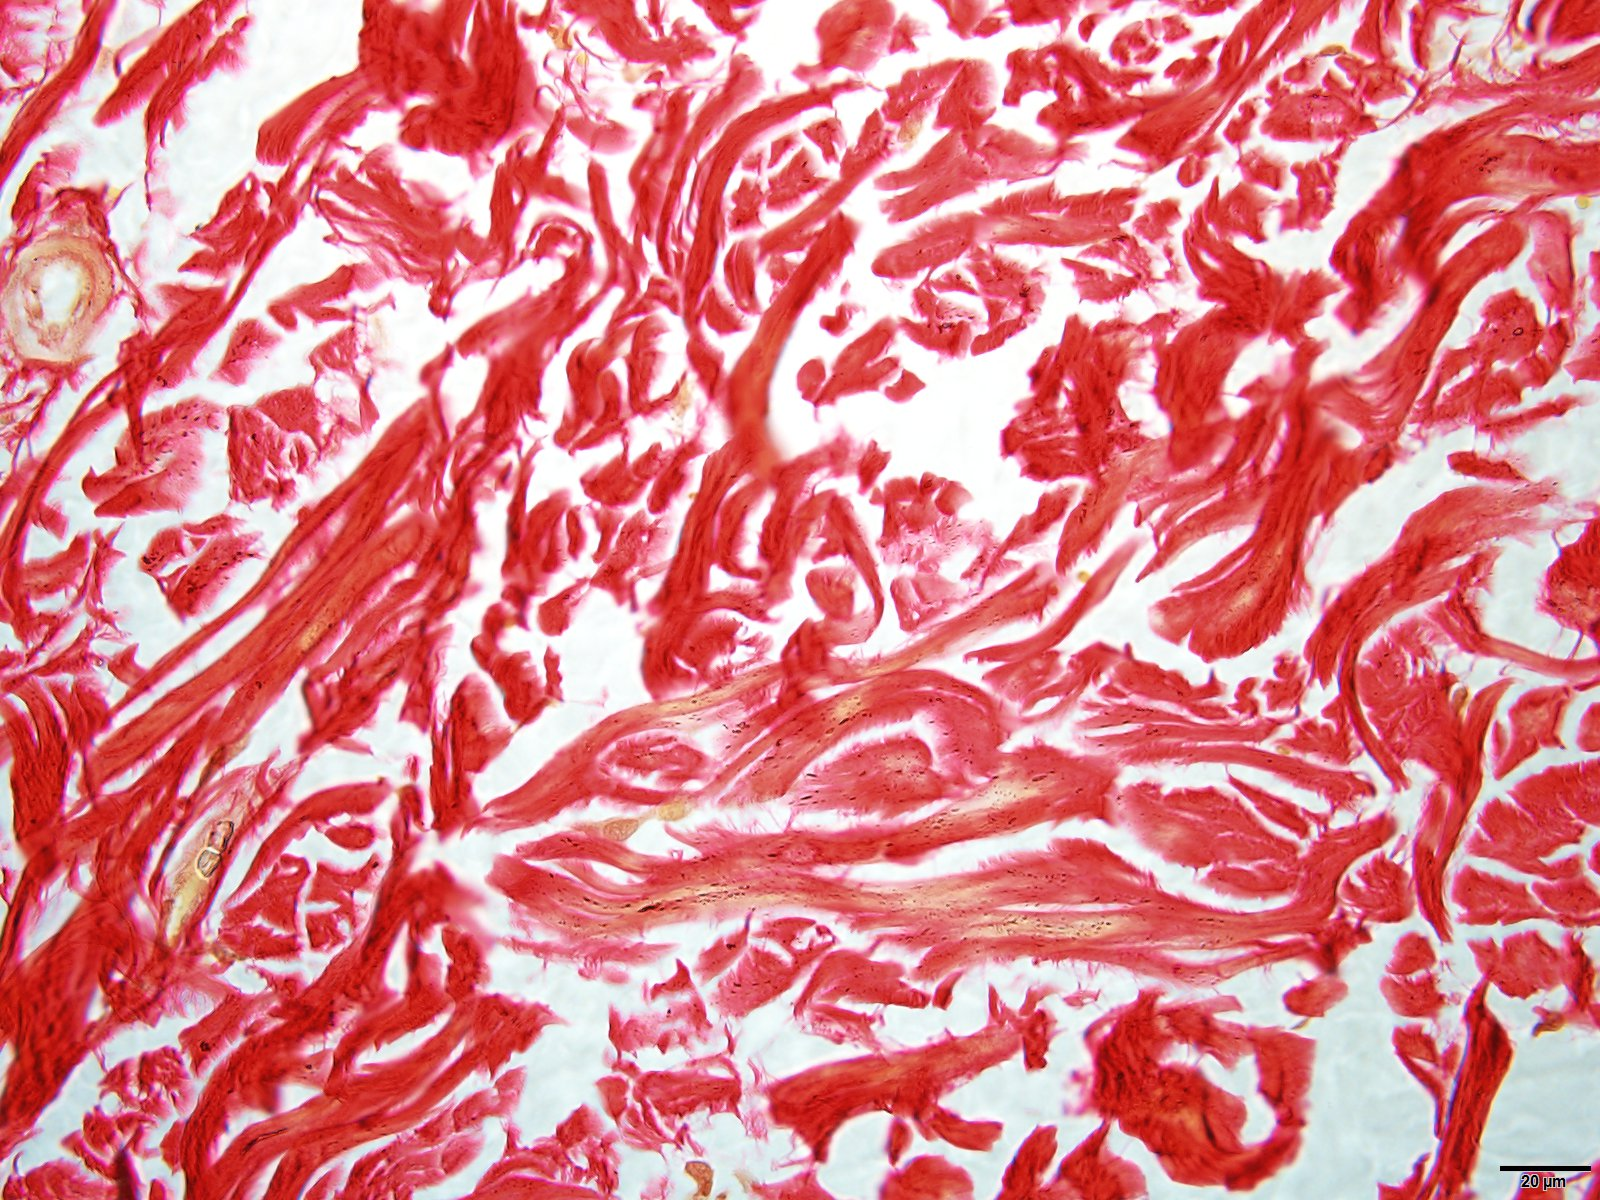
\includegraphics[scale=0.10]{3437_on_wrinkle_1.jpg}
%   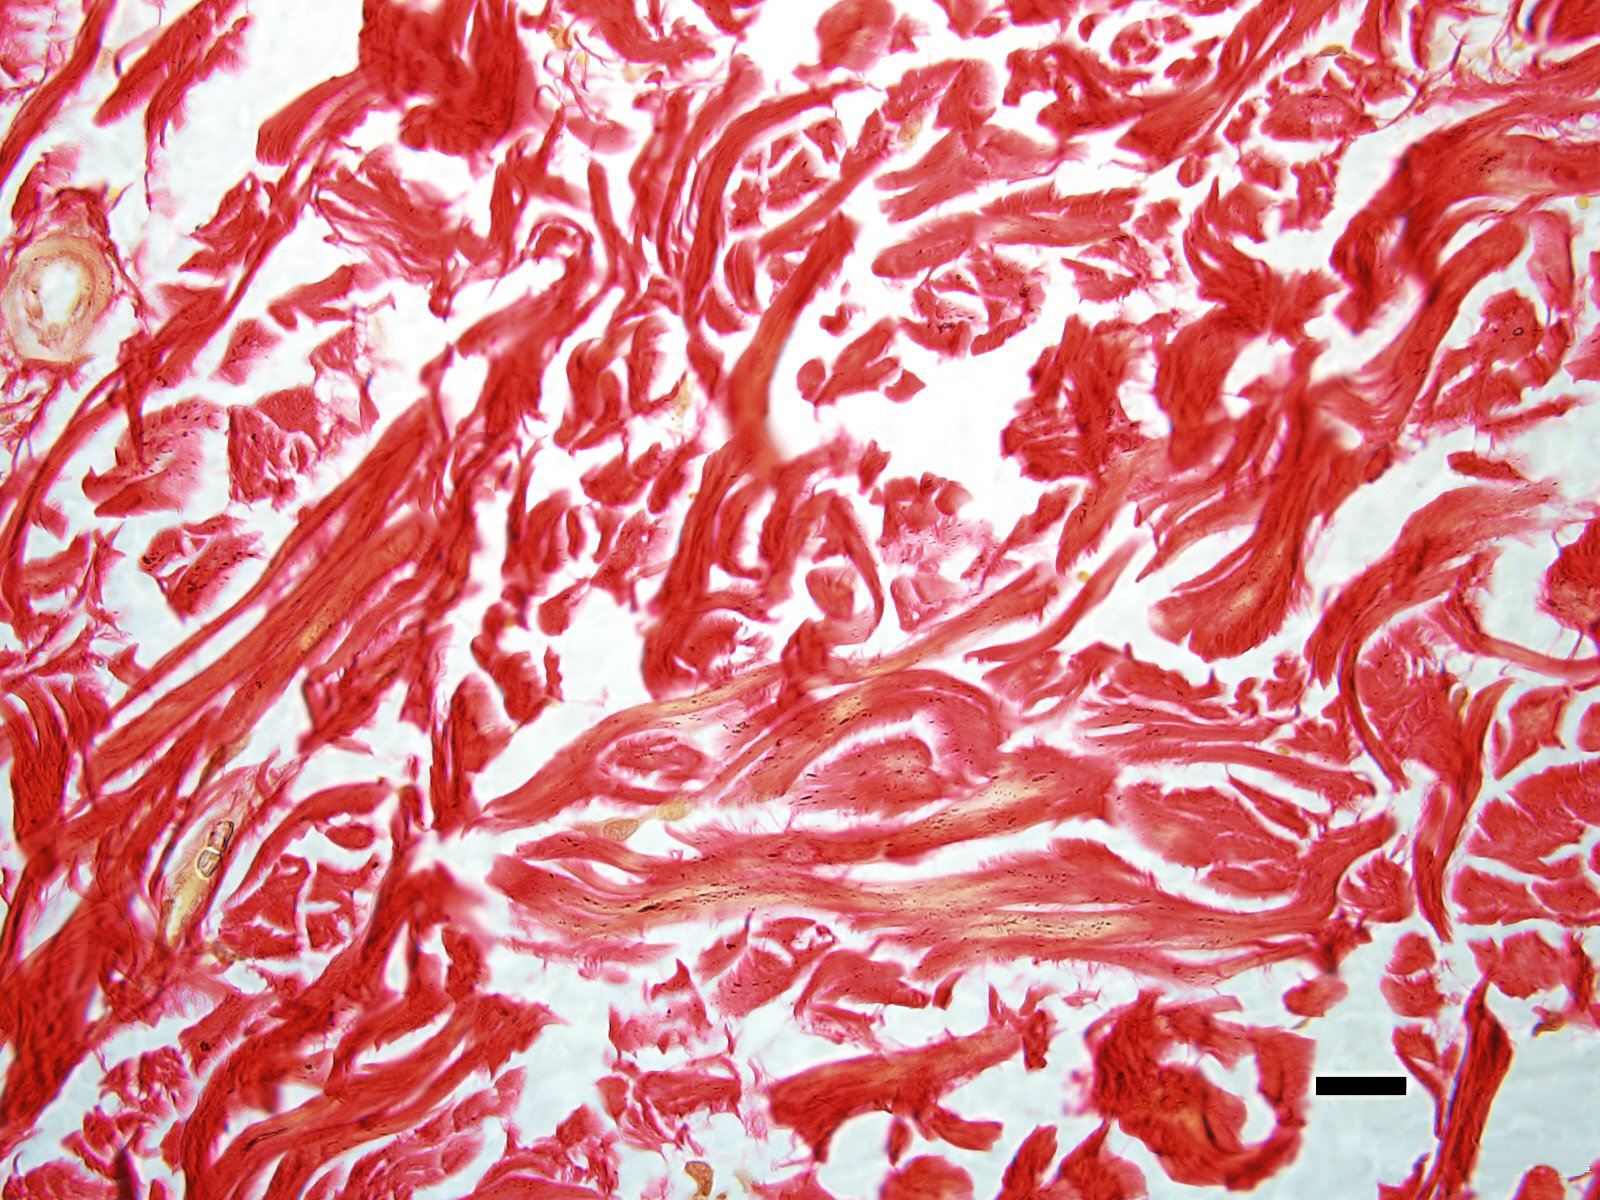
\includegraphics[scale=0.10]{fig5a.jpg}
    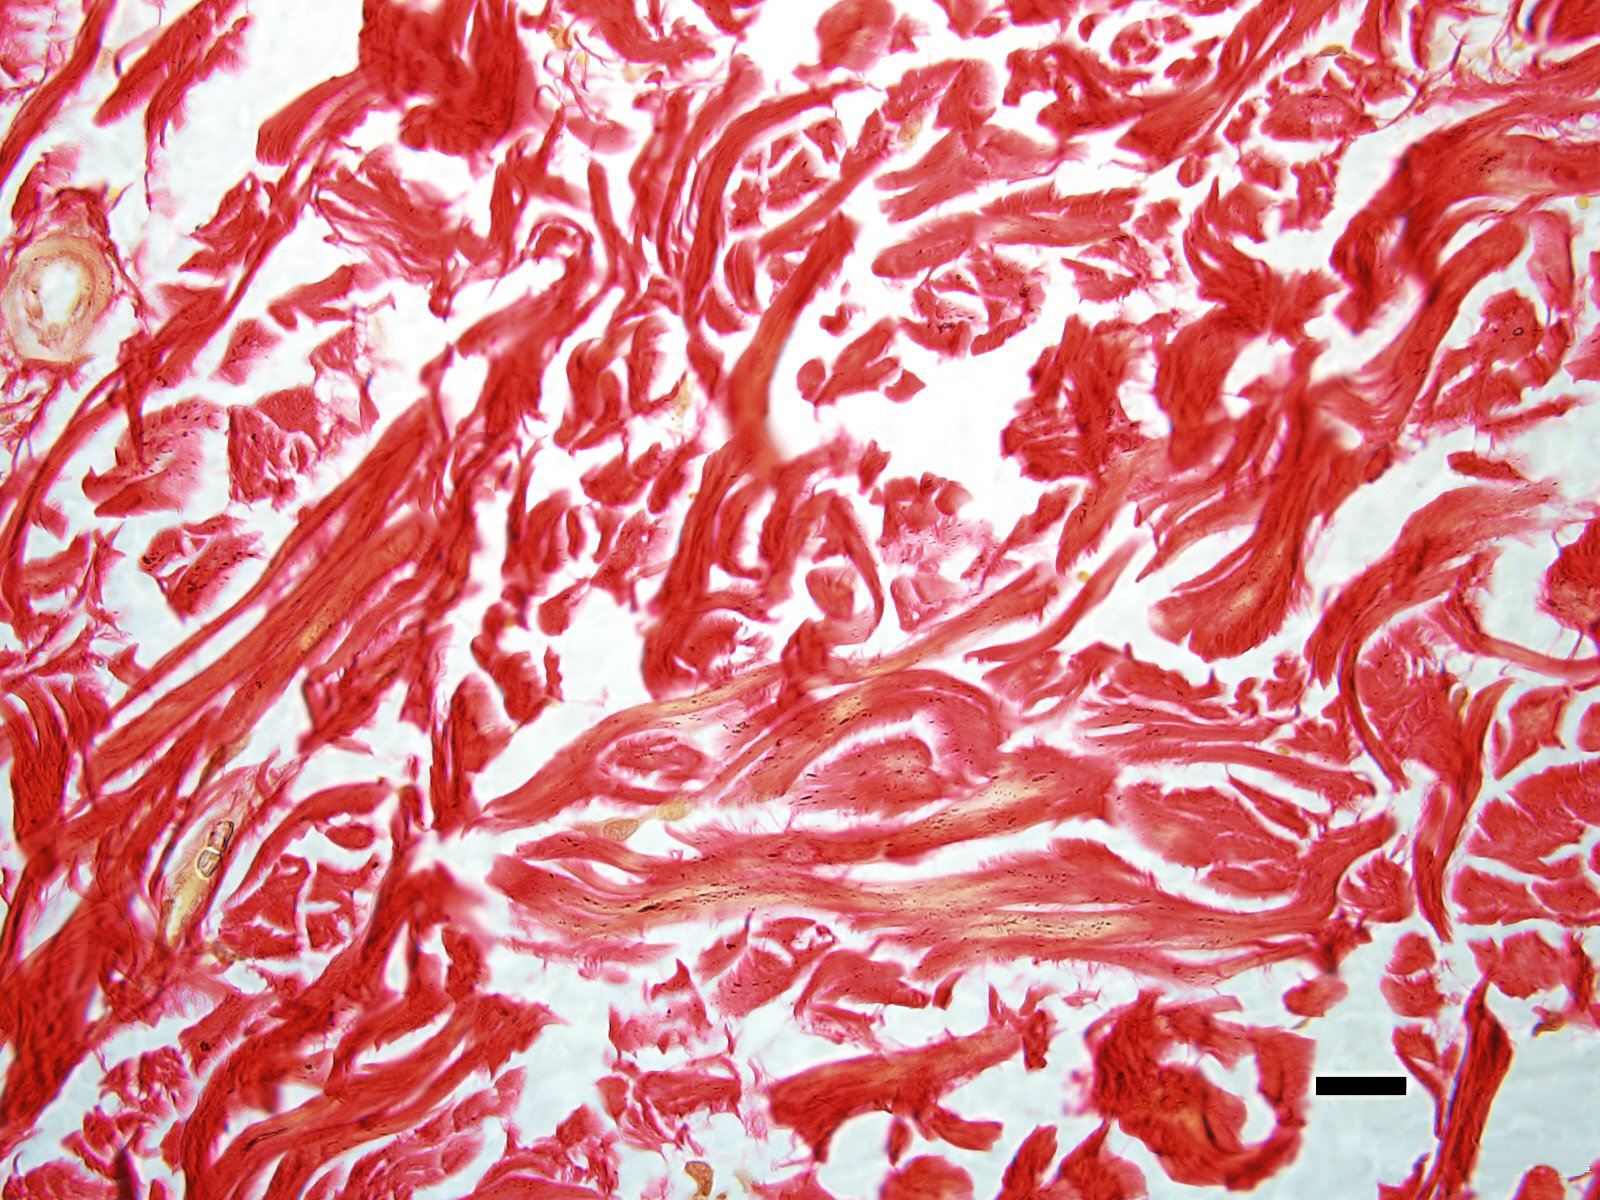
\includegraphics[width=0.46\textwidth]{fig5a.jpg}
% 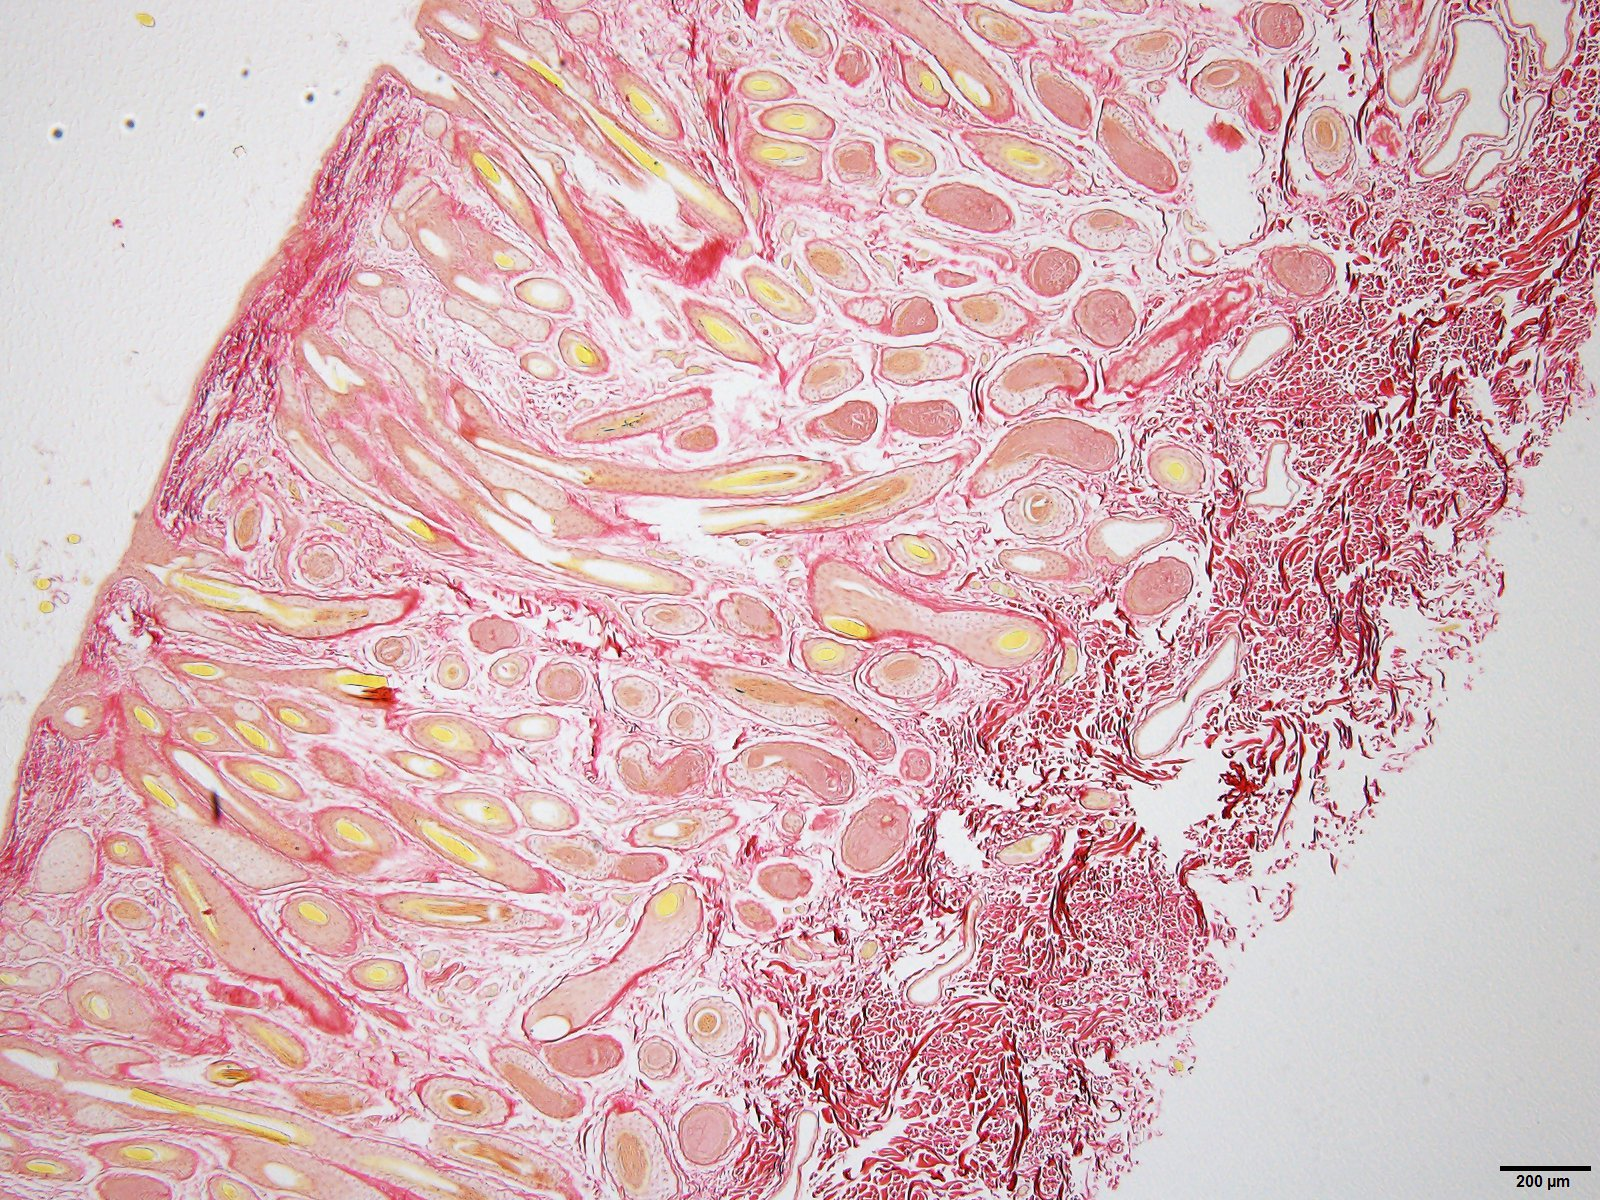
\includegraphics[width=1.0\textwidth]{w479-2-rigid.jpg}
  }
 \subfigure[Sheep 3457 Wrinkle-free]{
%   \label{fig:trial1he(ii)}
%   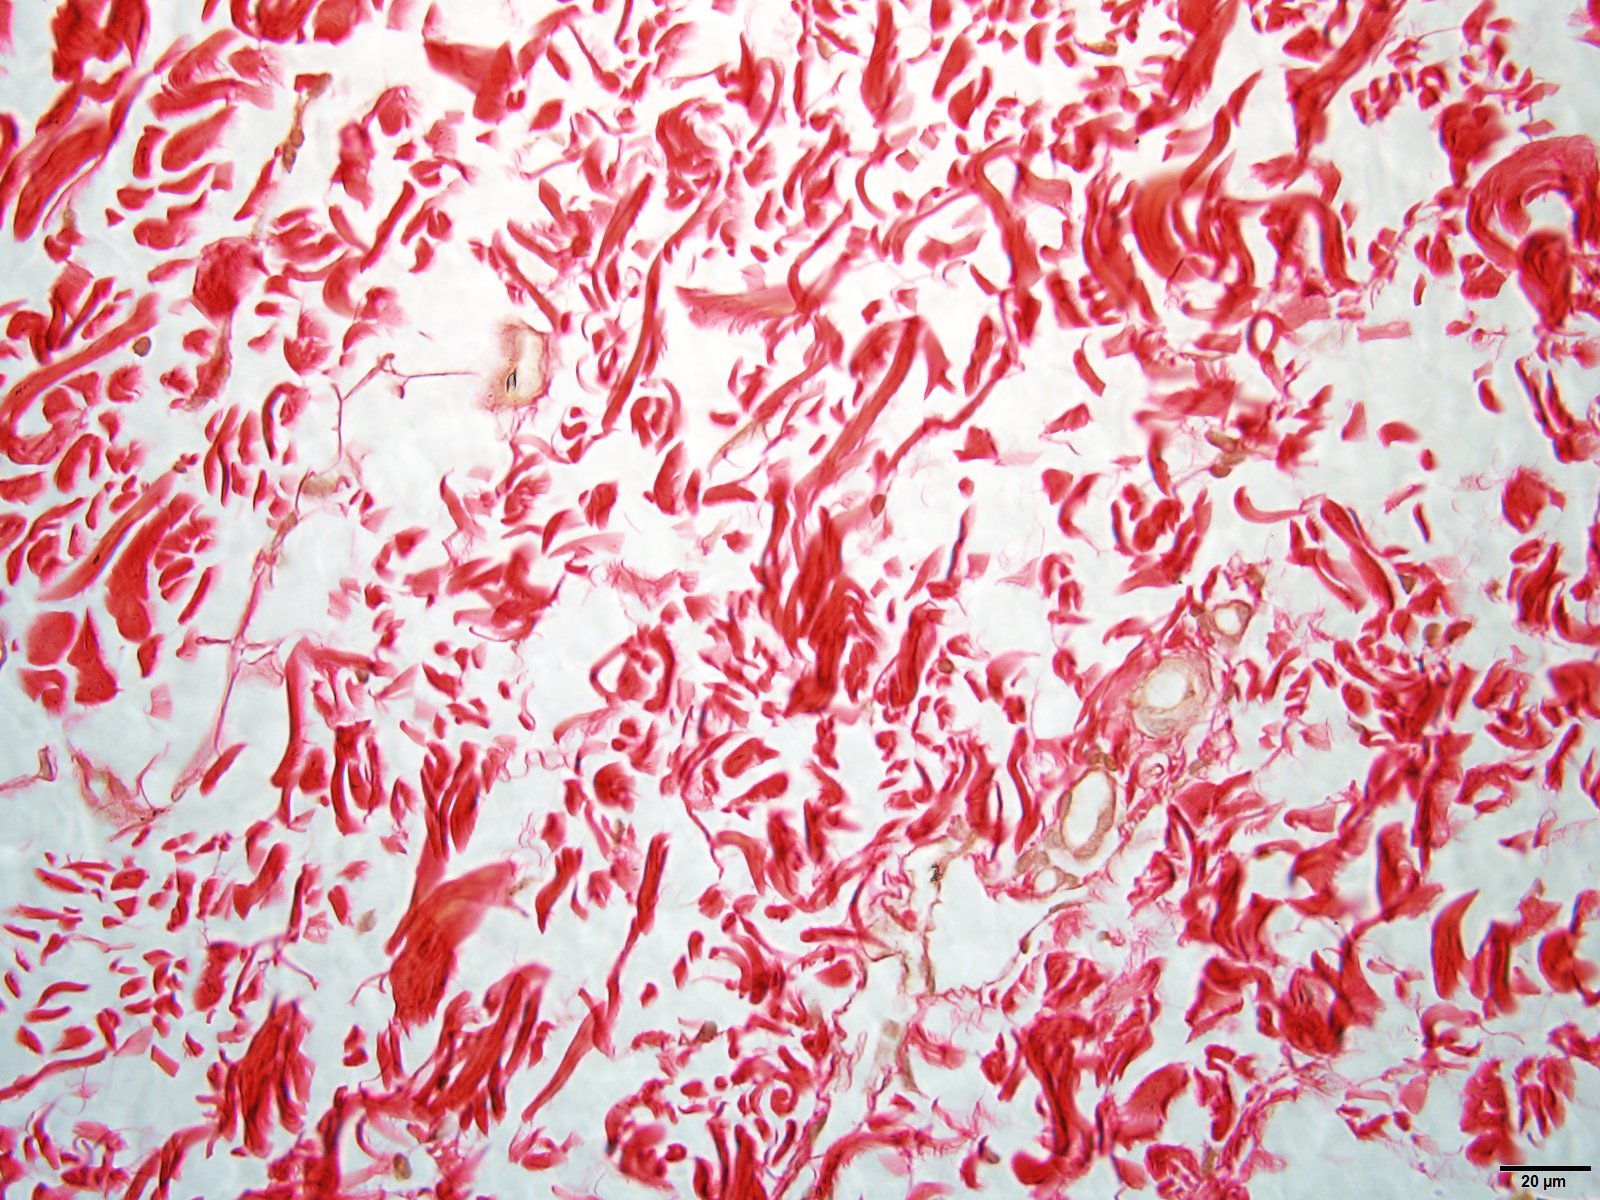
\includegraphics[scale=0.10]{3457_smooth_3.jpg}
%   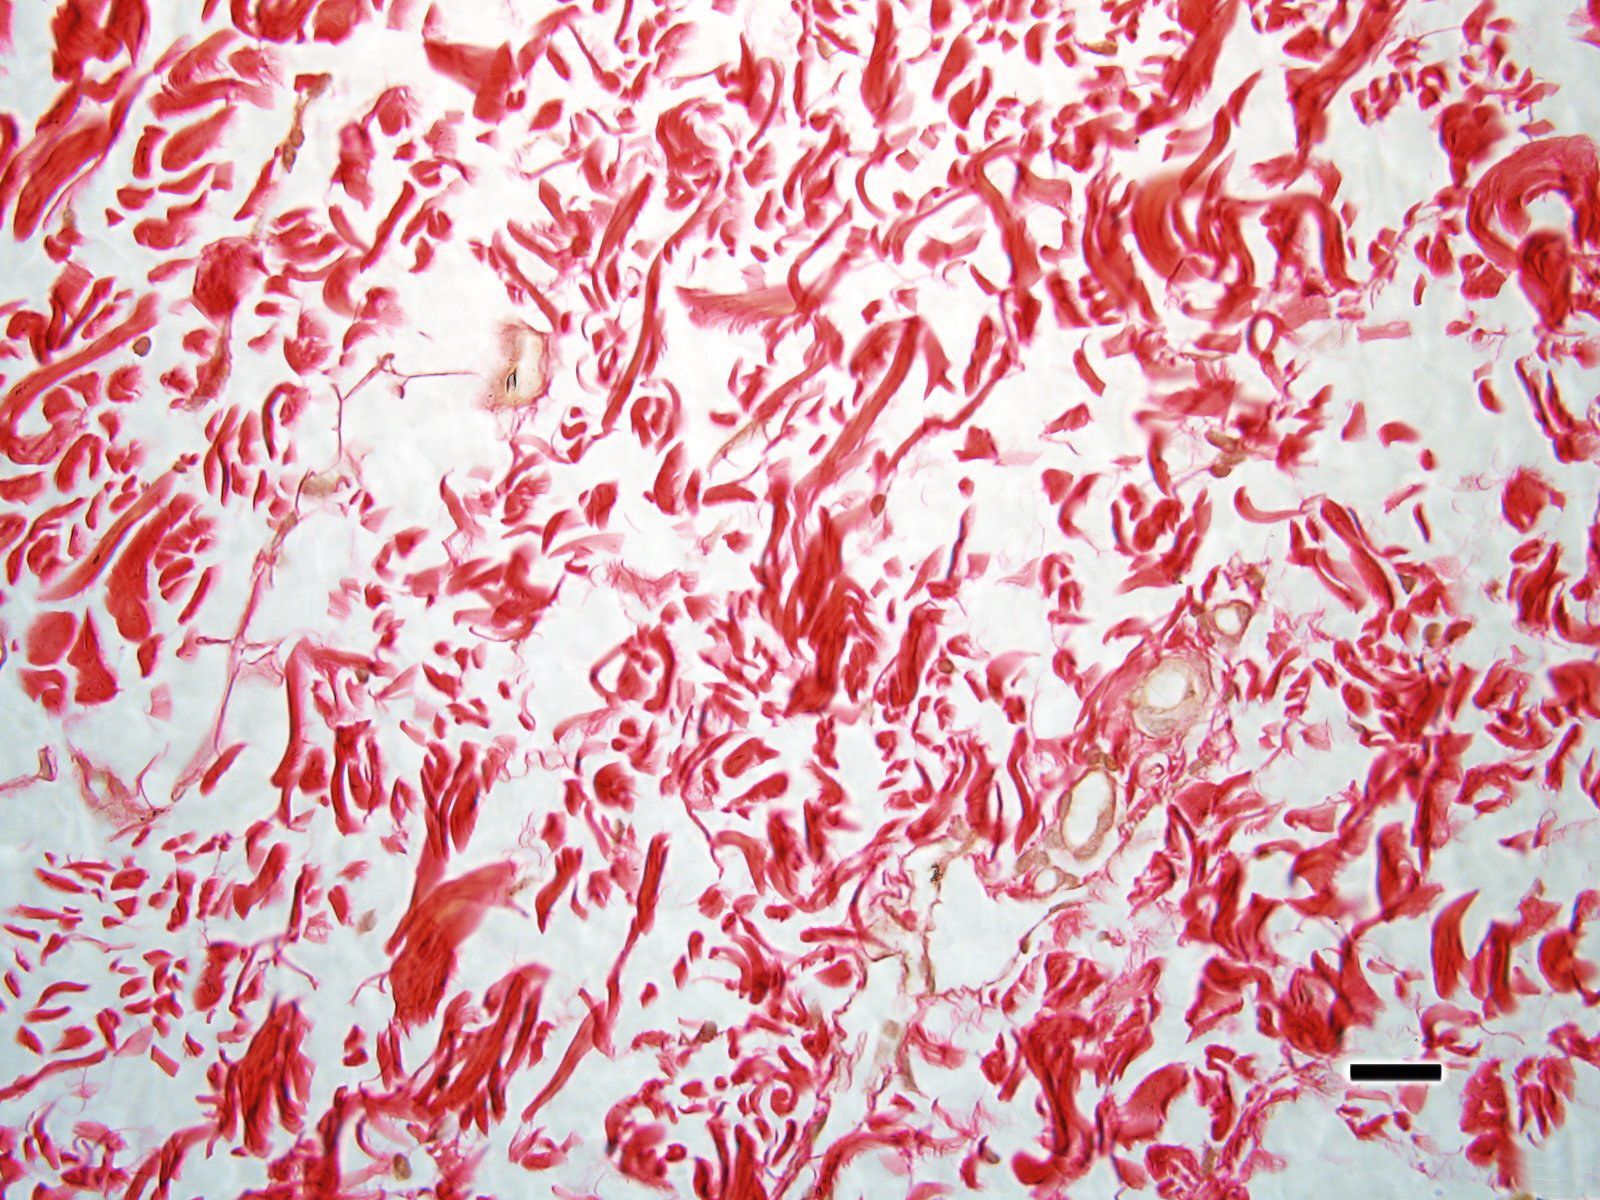
\includegraphics[scale=0.10]{fig5b.jpg}
    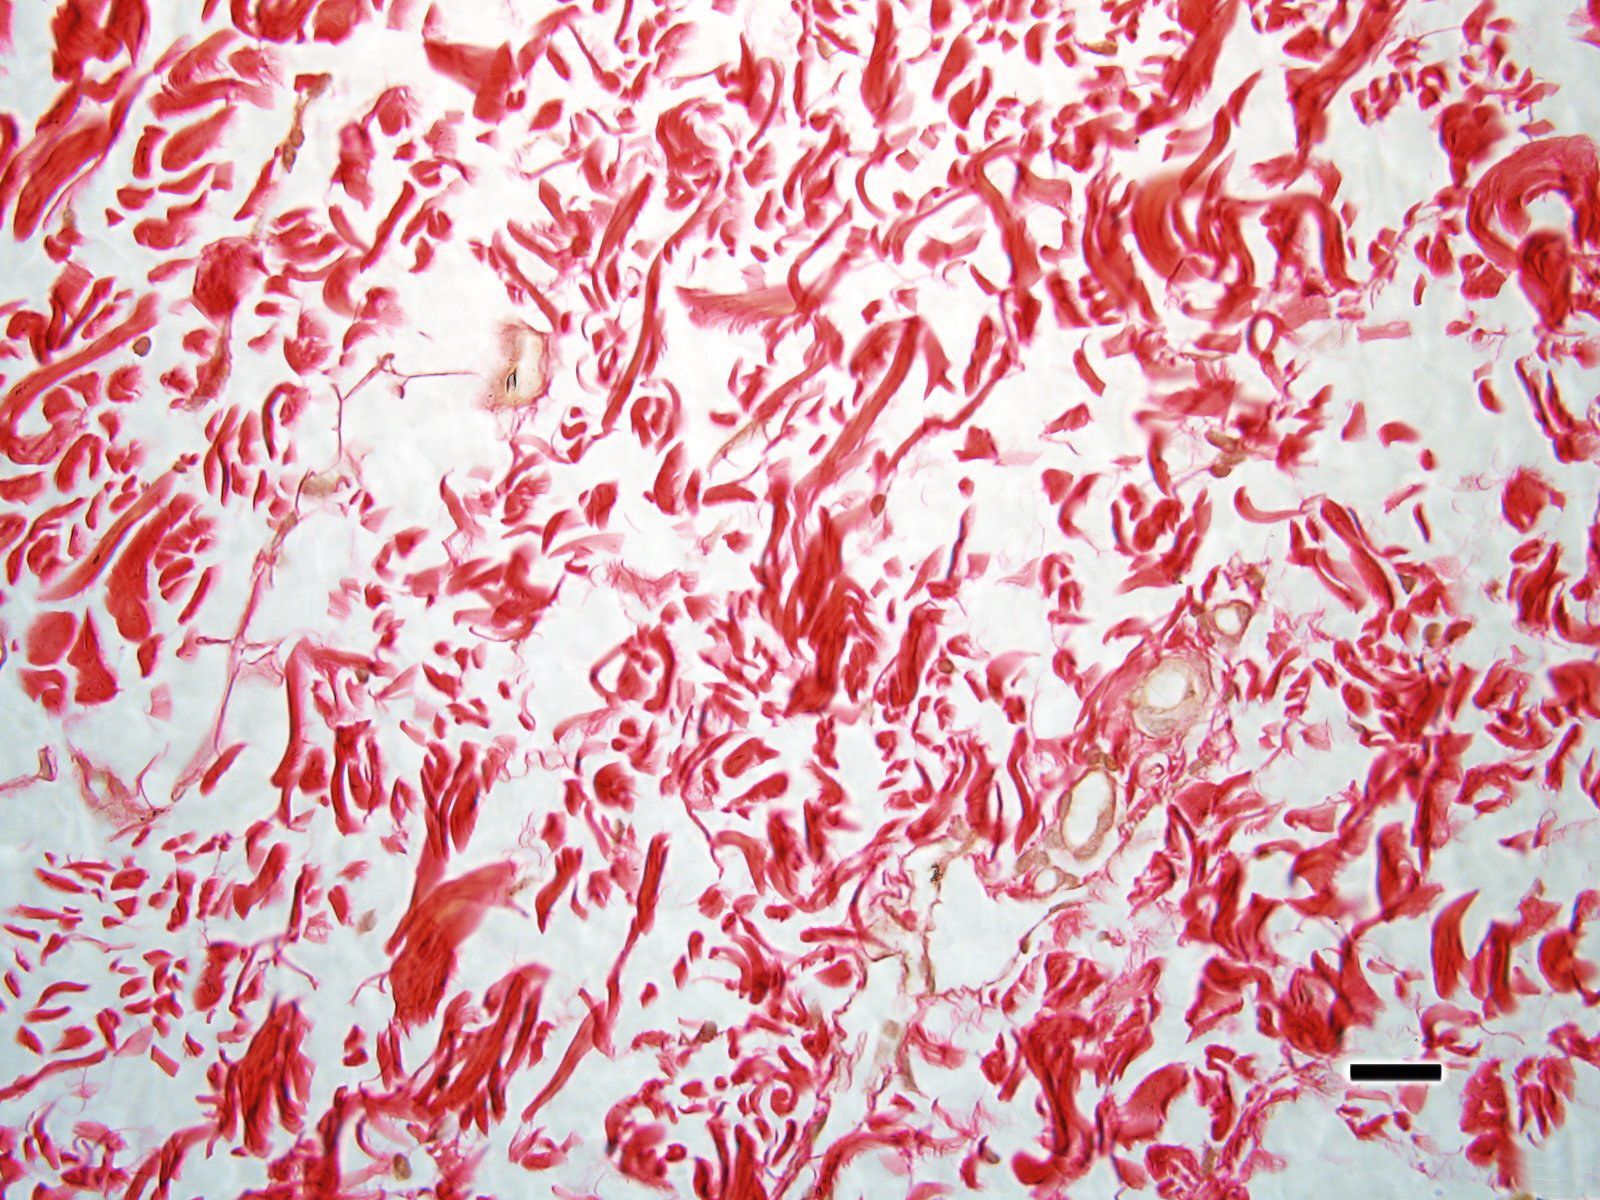
\includegraphics[width=0.46\textwidth]{fig5b.jpg}
  }
  \caption{Fields chosen at random from within Layer 3 (subpapillary dermis) of a wrinkled (a) and a wrinkle-free (b) sheep. Illustrates difference in collagen amount and structure. Stained with PSR and viewed with a 40x objective. Scale bar is $20\mu m$.}
\vfill
  \label{fig:psr40x}
\end{figure}

%\end{document}


The two fields shown in Figure~\ref{fig:psr40x} illustrate the difference between wrinkled and wrinkle-free sheep. They show that collagen in Layer 3 of wrinkled sheep is in larger (thicker and longer) aggregates (bundles of collagen fibres) and collagen within each bundle is more dense. So the collagen bundles in Figure~\ref{fig:psr40x}(a) take up considerably more 3 dimensional space than those on Figure~\ref{fig:psr40x}(b). More collagen is therefore present in wrinkled sheep. This was confirmed  with quantitative data.

 Image analysis was used to assess total amount of red stained pixels in each field.  The sum of calibrated optical densities of all pixels in the red image was calculated. Integrated optical density for each sheep is shown  in Figure~\ref{fig:redpixt1} for Trial 1 and Figure~\ref{fig:redpixt2} for Trial 2.
%\documentclass{article}
%\usepackage{graphicx,subfigure}
%\begin{document}

\begin{figure}[!h]
  \centering
  \captionsetup{width=0.6\textwidth}
% 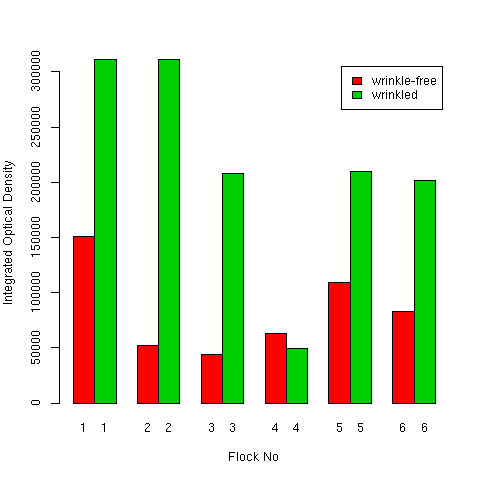
\includegraphics[width=0.8\textwidth]{t1odmeans.png}
  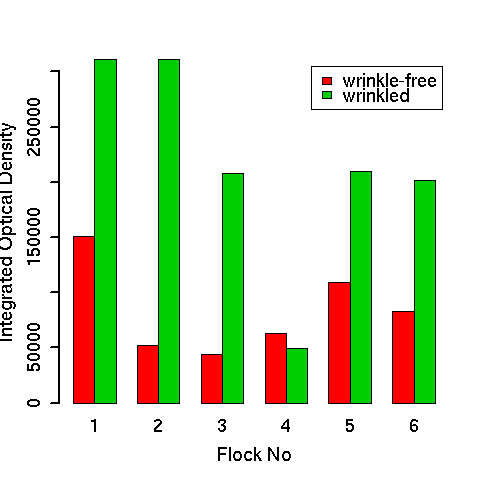
\includegraphics[width=0.6\textwidth]{newfig6.png}
  \caption{Integrated optical density of the red images of sections stained with PSR for each sheep in Trial 1 averaged over five microscope fields}
  \label{fig:redpixt1}
\end{figure}

%\end{document}


%\documentclass{article}
%\usepackage{graphicx,subfigure}
%\usepackage{caption,rotating}
%\begin{document}

\begin{figure}[!h]
\centering
\captionsetup{width=0.6\textwidth}
 \subfigure[Flock No 1 of Trial 2]{
%   \label{fig:redpixt2(i)}
%   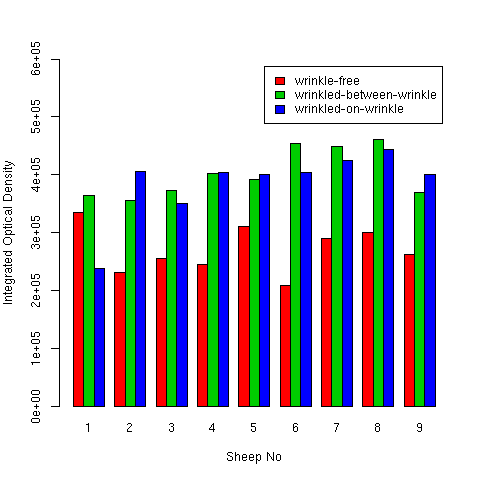
\includegraphics[scale=0.50]{t2f1odmeans.png}
%   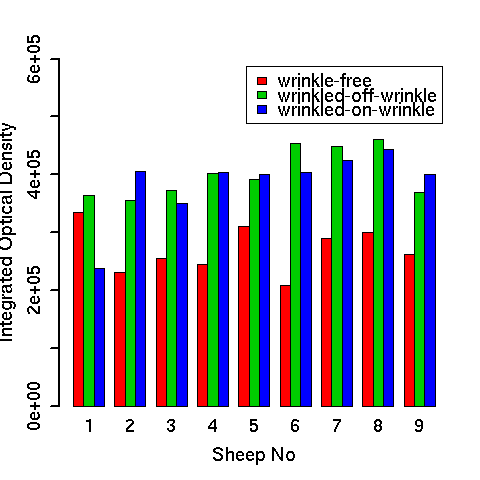
\includegraphics[scale=0.60]{newfig7a.png}
    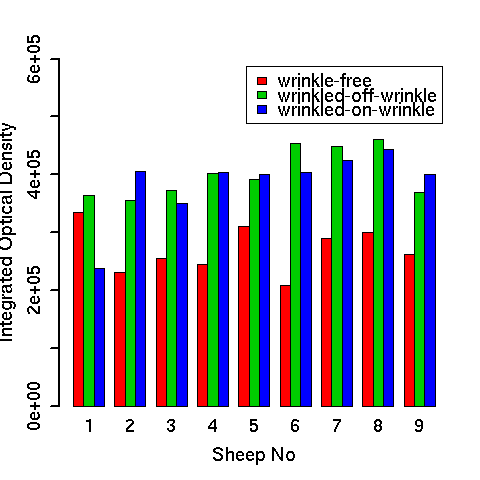
\includegraphics[width=0.60\textwidth]{newfig7a.png}
% 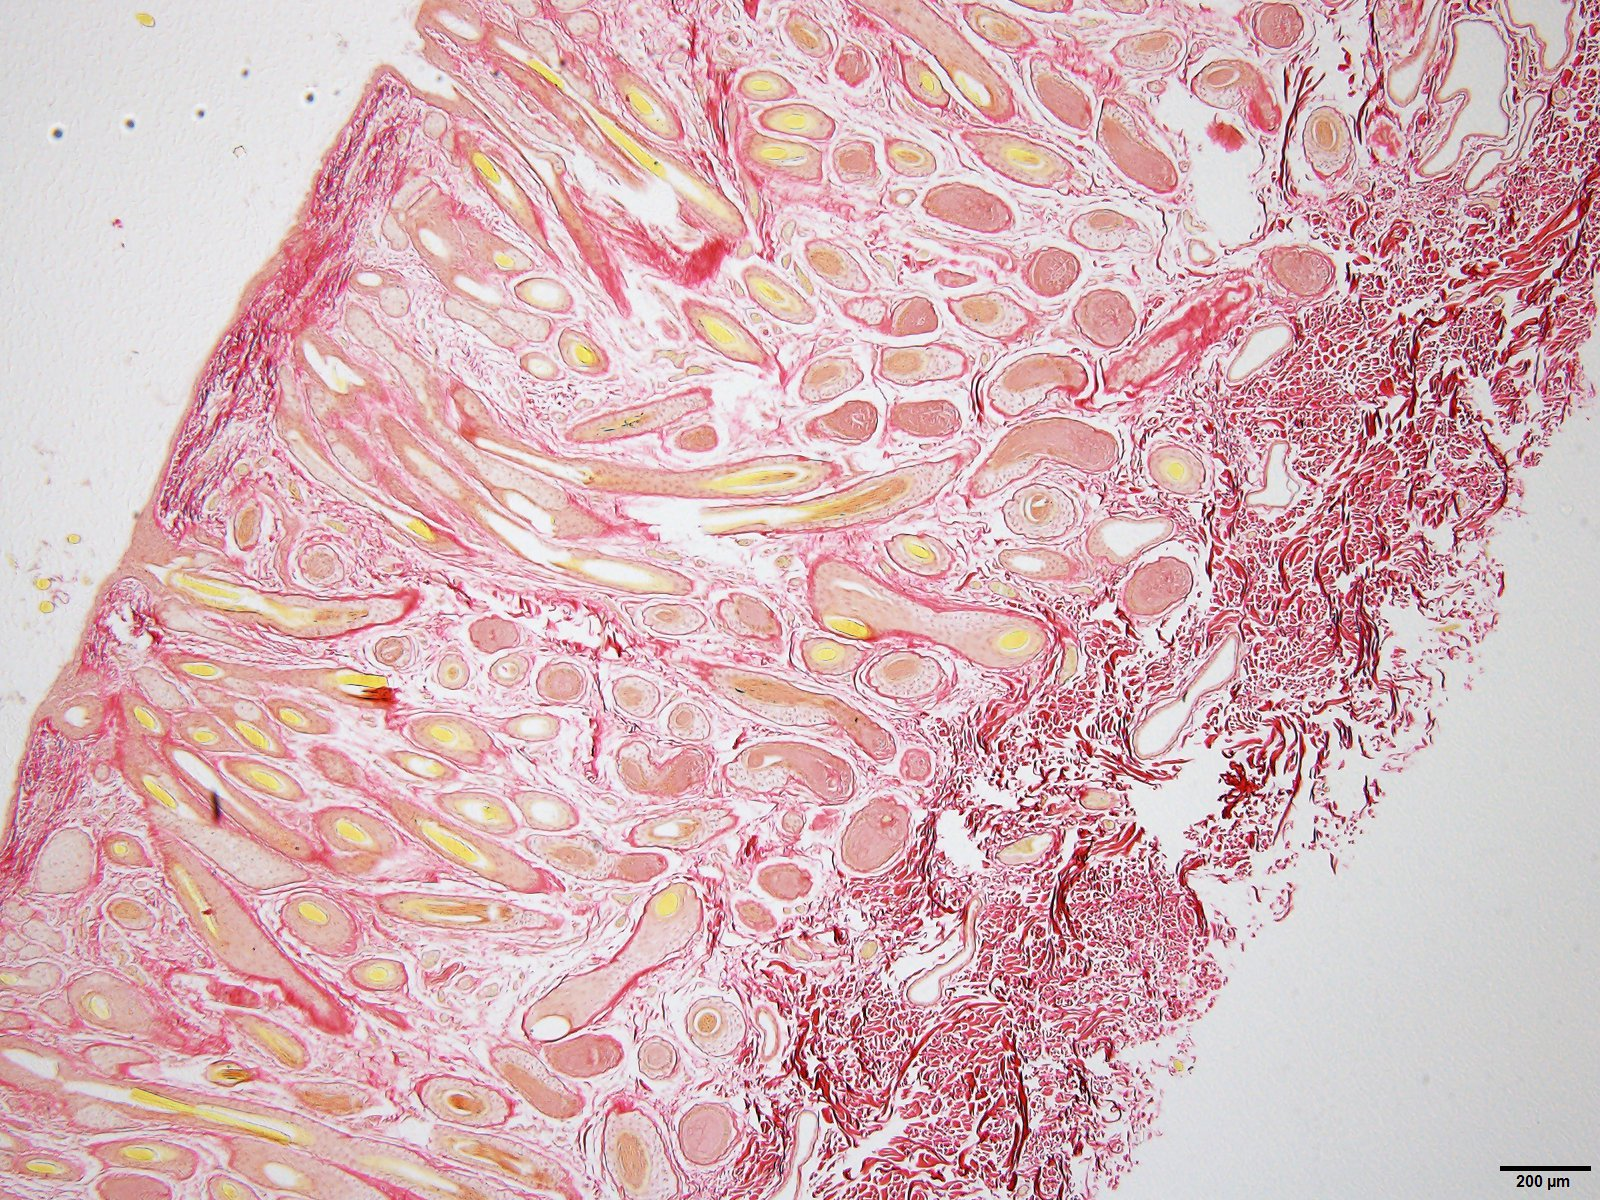
\includegraphics[width=1.0\textwidth]{w479-2-rigid.jpg}
  }
 \subfigure[Flock No 2  of Trial 2]{
%   \label{fig:redpixt2(ii)}
%   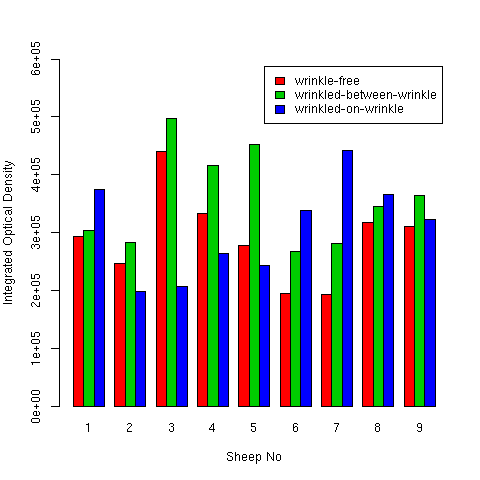
\includegraphics[scale=0.50]{t2f2odmeans.png}
%   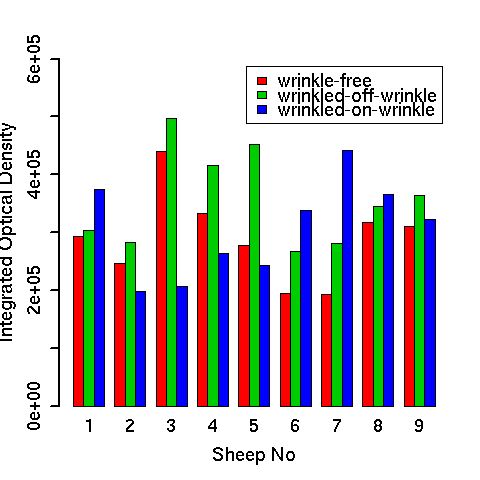
\includegraphics[scale=0.60]{newfig7b.png}
    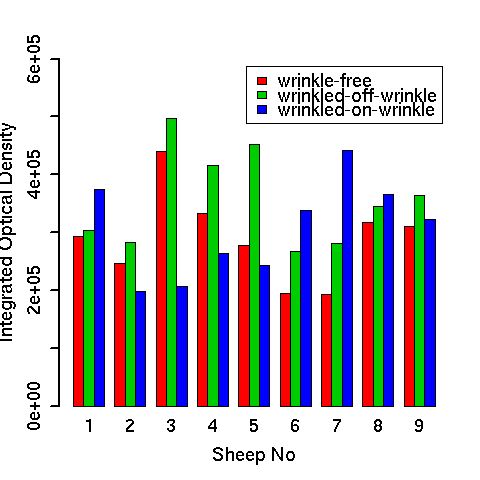
\includegraphics[width=0.60\textwidth]{newfig7b.png}
  }
  \caption{Integrated optical density of the red images of sections stained with PSR for each of the nine sheep in each Flock of Trial 2, averaged over five microscope fields}
\vfill
  \label{fig:redpixt2}
\end{figure}

%\end{document}


These data are a measure of total amount of collagen tissue present in the microscope section at the position of the chosen field in the lower dermis.
Total number of pixels in an image taken with a 40x objective was 1920000, so one could scale these optical density sums to average optical density of a pixel by dividing by 1920000. 
We can see that for Trial 1 wrinkle-free sheep always had less collagen, except for those in Flock 4. In Trial 2  wrinkle-free sheep always had less collagen than the off-wrinkle sample from wrinkled sheep, but the on-wrinkle sample was more variable.

Significance of differences apparent in Figure~\ref{fig:redpixt1} was tested by analysis of variance extracting terms for FlockNo, SkinType, and their interaction, as presented in Table~\ref{tab:redpixelt1aov}.
% latex table generated in R 3.4.2 by xtable 1.8-2 package
% Mon Jul 15 21:10:57 2019
\begin{table}[ht]
\centering
\caption{Analysis of variance of red pixel counts for Trial 1}
\label{tab:redpixelt1aov}
\begin{tabular}{lrrrrr}
  \hline
 & Df & Sum Sq & Mean Sq & F value & Pr($>$F) \\ 
  \hline
FlockNo & 1 & 48141986950.46 & 48141986950.46 & 9.87 & 0.0027 \\ 
  SkinType & 1 & 259320673232.61 & 259320673232.61 & 53.16 & 0.0000 \\ 
  FlockNo:SkinType & 1 & 26844676679.26 & 26844676679.26 & 5.50 & 0.0225 \\ 
  Residuals & 56 & 273170345102.88 & 4878041876.84 &  &  \\ 
   \hline
\end{tabular}
\end{table}


The residual term in Table~\ref{tab:redpixelt1aov} is variation between randomly chosen Fields within a specimen, because there were no replicate sheep within each Flock:SkinType subclass. The difference between wrinkled and wrinkle-free SkinTypes is significant at 5\% level. Flock differences are not significant. An interaction was significant.

The equivalent analysis of variance for Trial 2 (Figure~\ref{fig:redpixt2}) data is shown in Table~\ref{tab:redpixelt2aov}.
% latex table generated in R 3.4.2 by xtable 1.8-2 package
% Wed Jul 24 20:43:14 2019
\begin{table}[ht]
\centering

\caption{Analysis of variance of red pixel optical density sums for Trial 2}
\label{tab:redpixelt2aov}

\begin{tabular}{lrrrrr}
  \hline
 & Df & Sum Sq & Mean Sq & F value & Pr($>$F) \\ 
  \hline
FlockNo                  & 1 & 91548864255.47 & 91548864255.47 & 37.41 & 0.0000 \\ 
  SkinType                 & 1 & 412338258758.73 & 412338258758.73 & 168.48 & 0.0000 \\ 
  SampPos                  & 1 & 50325174039.48 & 50325174039.48 & 20.56 & 0.0000 \\ 
  FlockNo:SkinType         & 1 & 101676878442.96 & 101676878442.96 & 41.55 & 0.0000 \\ 
  FlockNo:SkinType:SheepNo & 49 & 1081769314333.64 & 22076924782.32 & 9.02 & 0.0000 \\ 
  Residuals                & 218 & 533522617623.69 & 2447351456.99 &  &  \\ 
   \hline
\end{tabular}
\end{table}


Differences between wrinkled and wrinkle-free SkinTypes are now shown to be highly significant. Flock differences were not significant and a significant interaction of Flock with SkinType was found.  

 The on-wrinkle and off-wrinkle sampling positions within wrinkled specimens were not significantly different. On-wrinkle specimens actually had a lower integrated optical density than off-wrinkle specimens indicating slightly less collagen on a wrinkle than between wrinkles.
There was also a significant amount of variation between sheep within the FlockNo and SkinType combinations. Sheep are much more variable than image Fields within a sheep, which is what the Residual term in Table~\ref{tab:redpixelt2aov} represents. In this analysis the Sheep term is the error term for all terms above it in the analysis of variance table, whereas Trial 1 had no sheep replication and we were forced to use the FlockNo:SkinType term as error. This explains why SkinType differences were less significant in Trial 1. 

Means and standard deviations for integrated optical density for both Trial 1 and Trial 2 are shown in Table~\ref{tab:redpixelodmeans}
%\documentclass{article}
%\usepackage{lscape}
%\begin{document}

\begin{table}[htp]
\centering
\caption{Means and standard errors for integrated red pixel optical density of wrinkled and wrinkle-free sheep in Trial 1 and Trial 2}
\label{tab:redpixelodmeans}
\vspace{0.1in}
\begin{tabular}{|p{0.5in}|p{0.6in}|p{1.0in}|p{1.0in}|p{1.0in}|}  \hline
     Trial & Parameter &  Wrinkle-free  &  Wrinkled (between-wrinkle) & Wrinkled (on-wrinkle)  \\ 
\hline
  1  & Mean &   83748        &   215232   &       \\
  1  & Standard deviation &   47535      &    98720   &  \\ \hline
  2  & Mean &   280851       &   380427    &  347170   \\ 
  2  & Standard deviation &    70609     &  75988  &  96787 \\ \hline
\end{tabular}
\end{table}

%\end{document}

We see that wrinkle-free sheep actually have quite a low amount of collagen in Trial 1. 
The Trial 2 sheep were from commercial flocks, and were generally more wrinkled than those of Trial 1.  Trial 2  wrinkled sheep ( either on-wrinkle or  off-wrinkle specimens) had a higher amount of collagen than wrinkled sheep from Trial 1. 

The data and analyses show that more collagen is present in the lower dermis of wrinkled sheep than wrinkle-free sheep.  The actual size of the difference varied from 2.5 x in Trial 1 to 1.4 x in Trial 2. 
Within wrinkled sheep we detected no difference in amount of collagen between samples taken on a wrinkle or in-between wrinkles.


\subsubsection{Spatial location and structure of collagen}
It has been established that wrinkled sheep have more collagen . We now investigate location of collagen in the dermis and whether arrangement of collagen fibres varies.
Figure~\ref{fig:he10x} shows images of layers 2 and 3 in specimens from two sheep, one being wrinkled (a off-wrinkle specimen) and one being wrinkle-free.
%\documentclass{article}
%\usepackage{graphicx,subfigure}
%\usepackage{caption,rotating}
%\begin{document}

\begin{figure}[!h]
\centering
\captionsetup{width=0.7\textwidth}
 \subfigure[Sheep 3453 Wrinkled]{
%    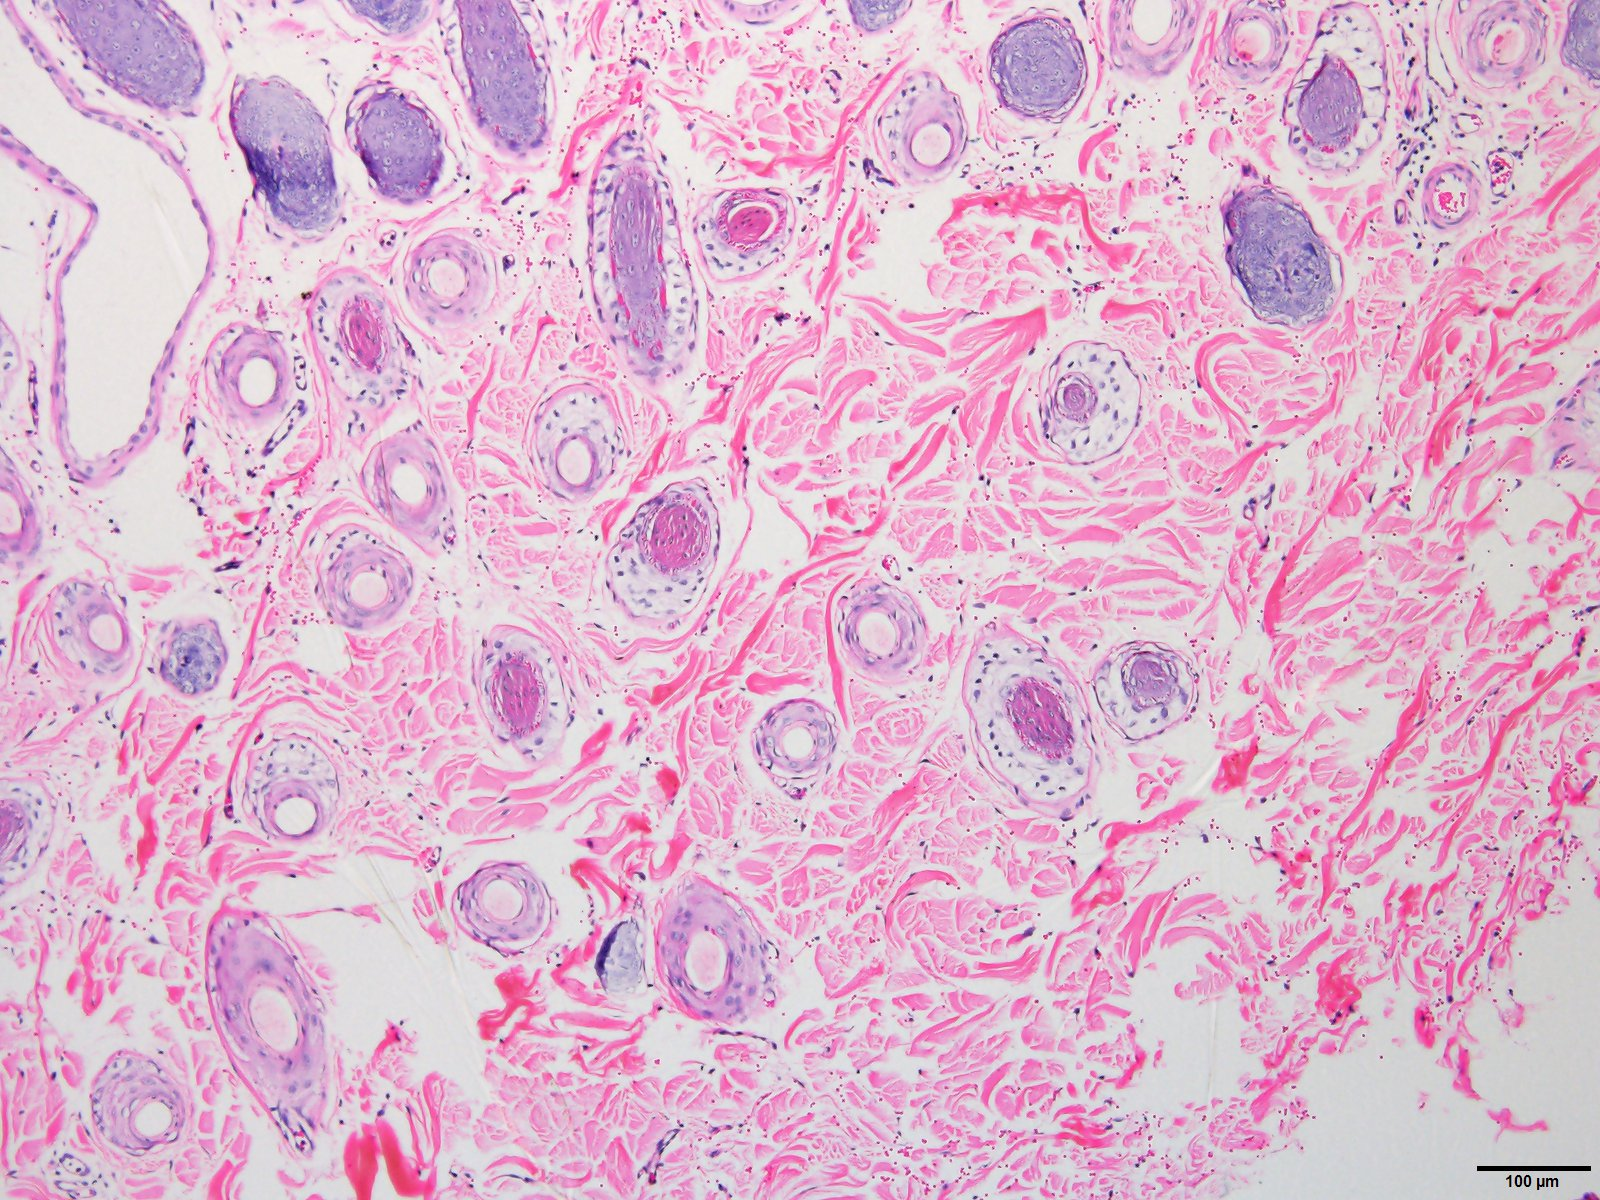
\includegraphics[scale=0.20]{3453_btwn_wrinkle_10x.jpg}
%   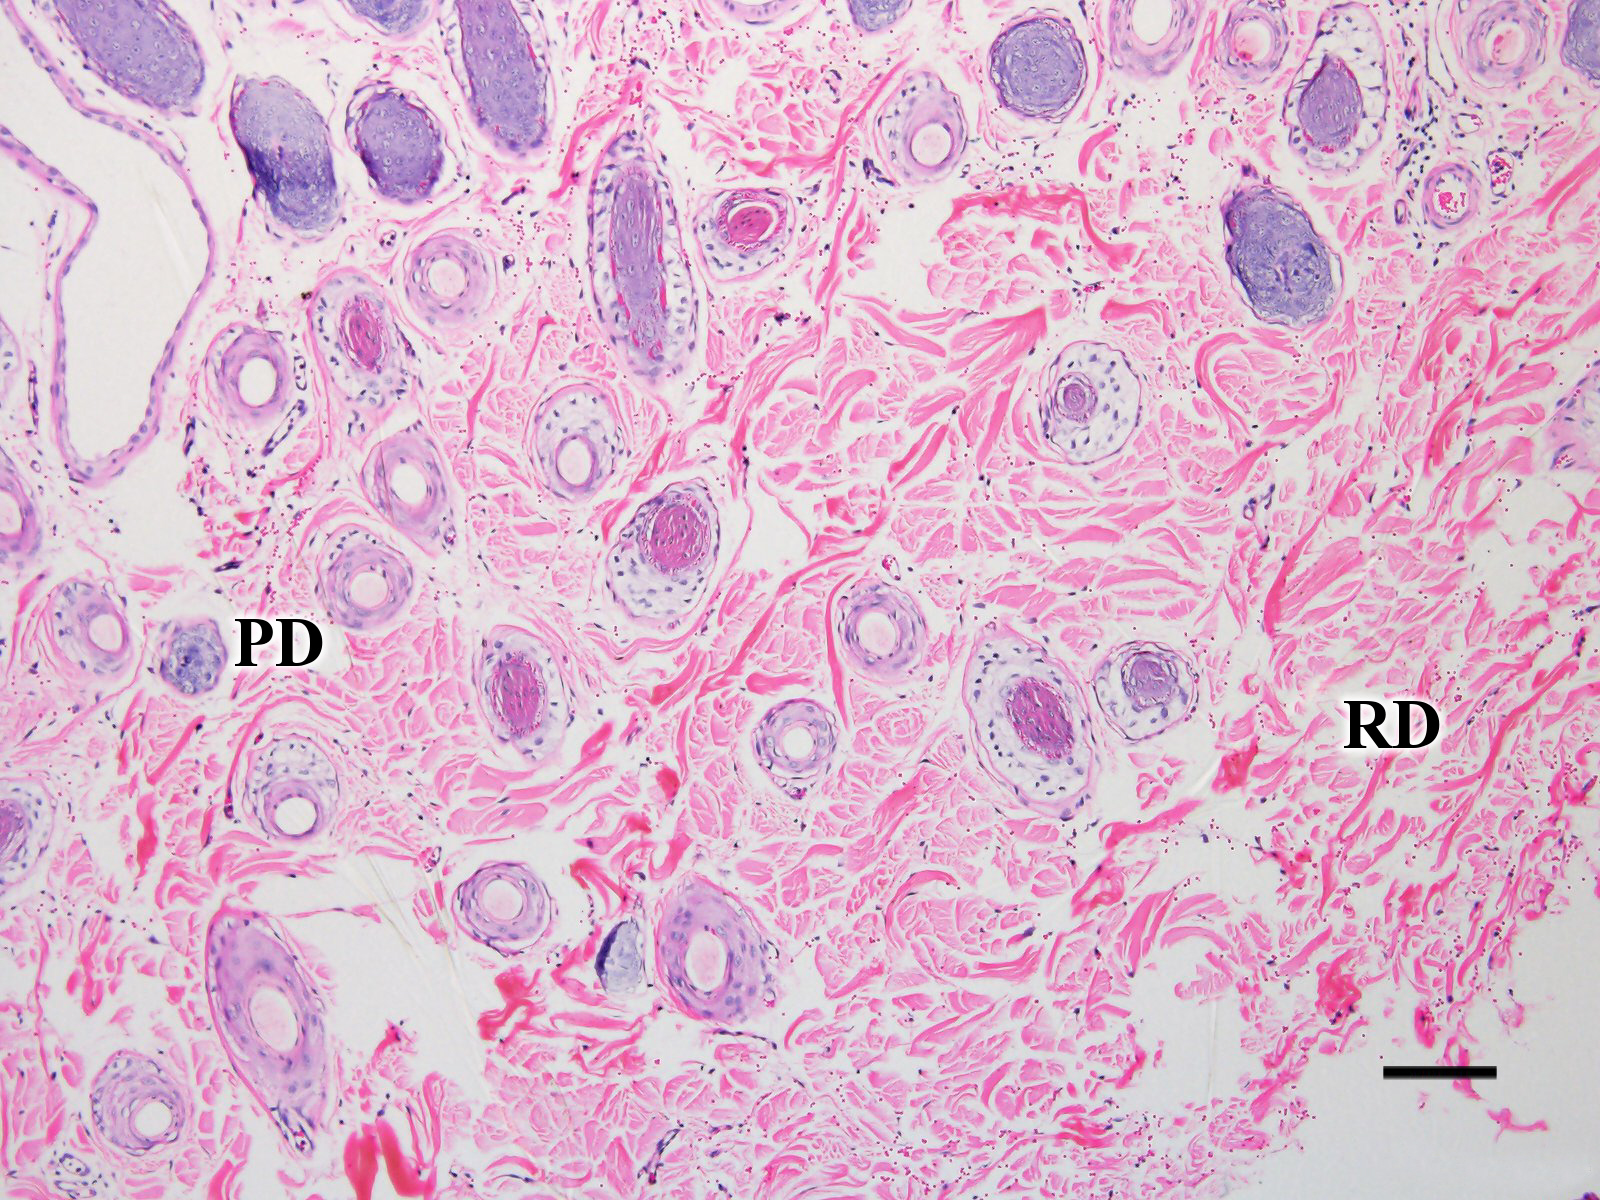
\includegraphics[scale=0.10]{fig8a.jpg}
    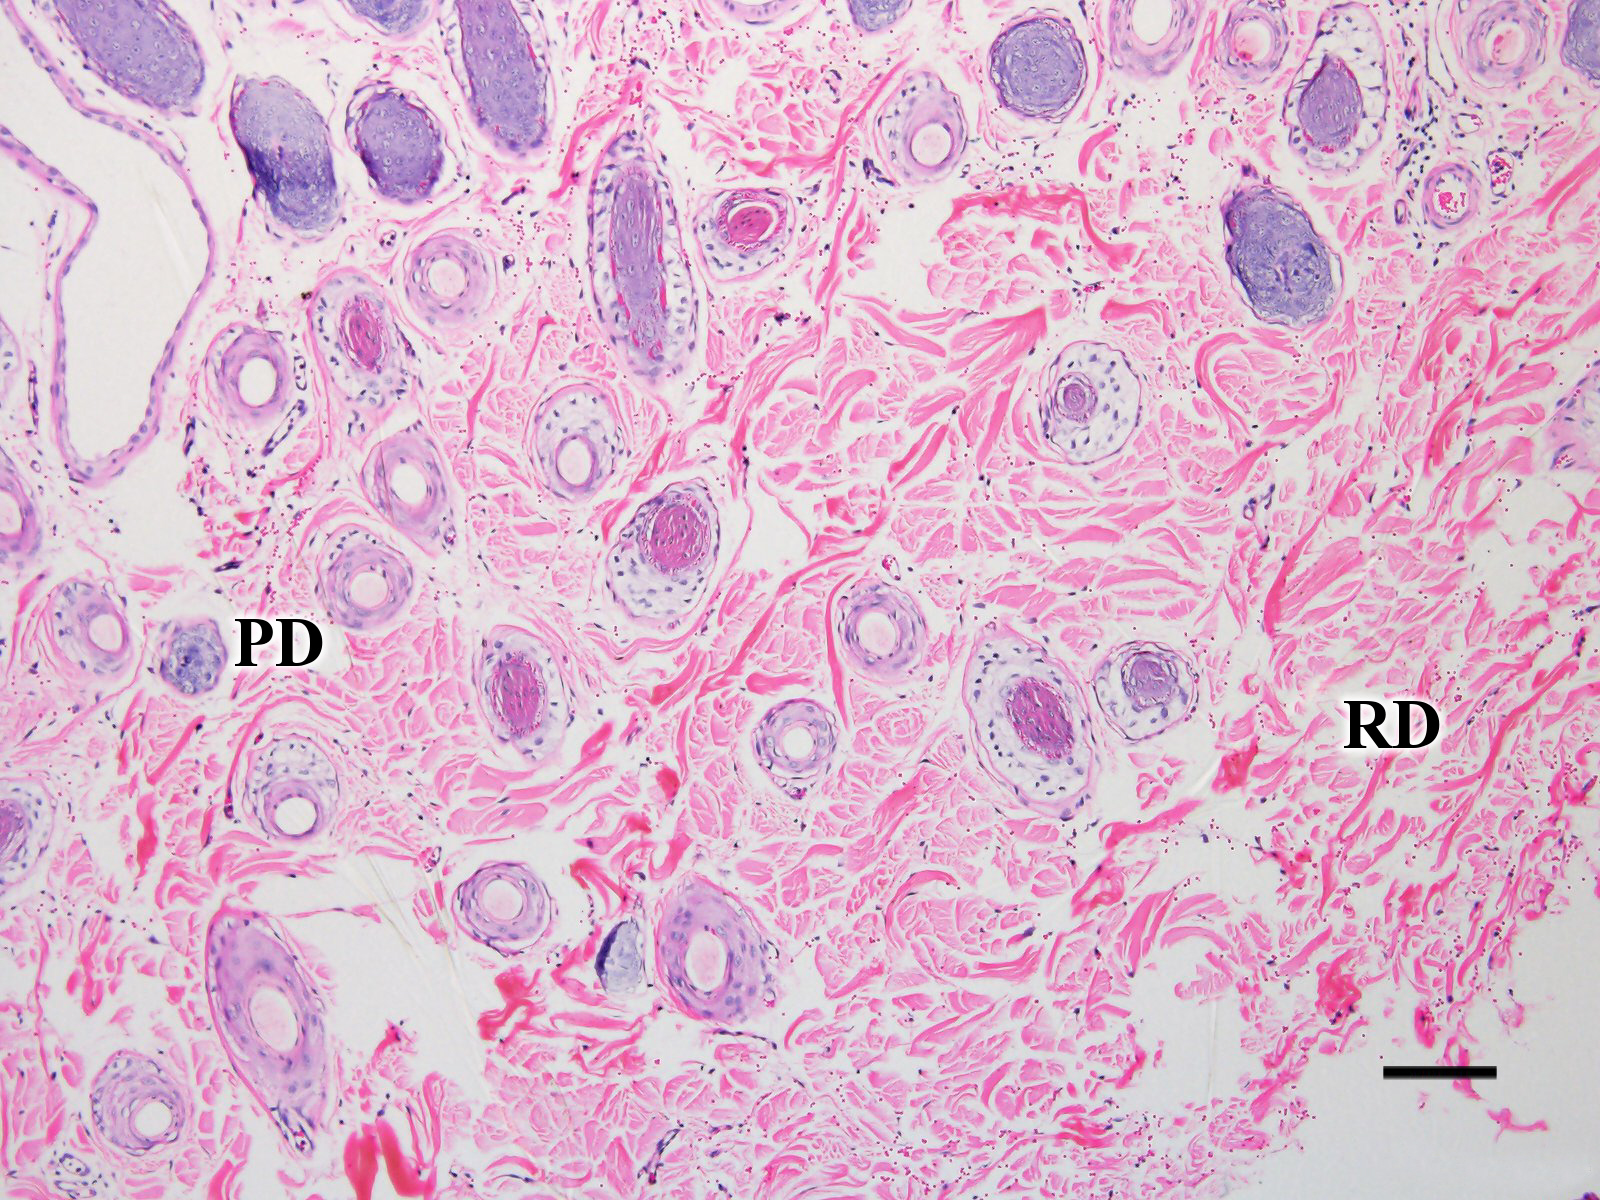
\includegraphics[width=0.7\textwidth]{fig8a.jpg}
% 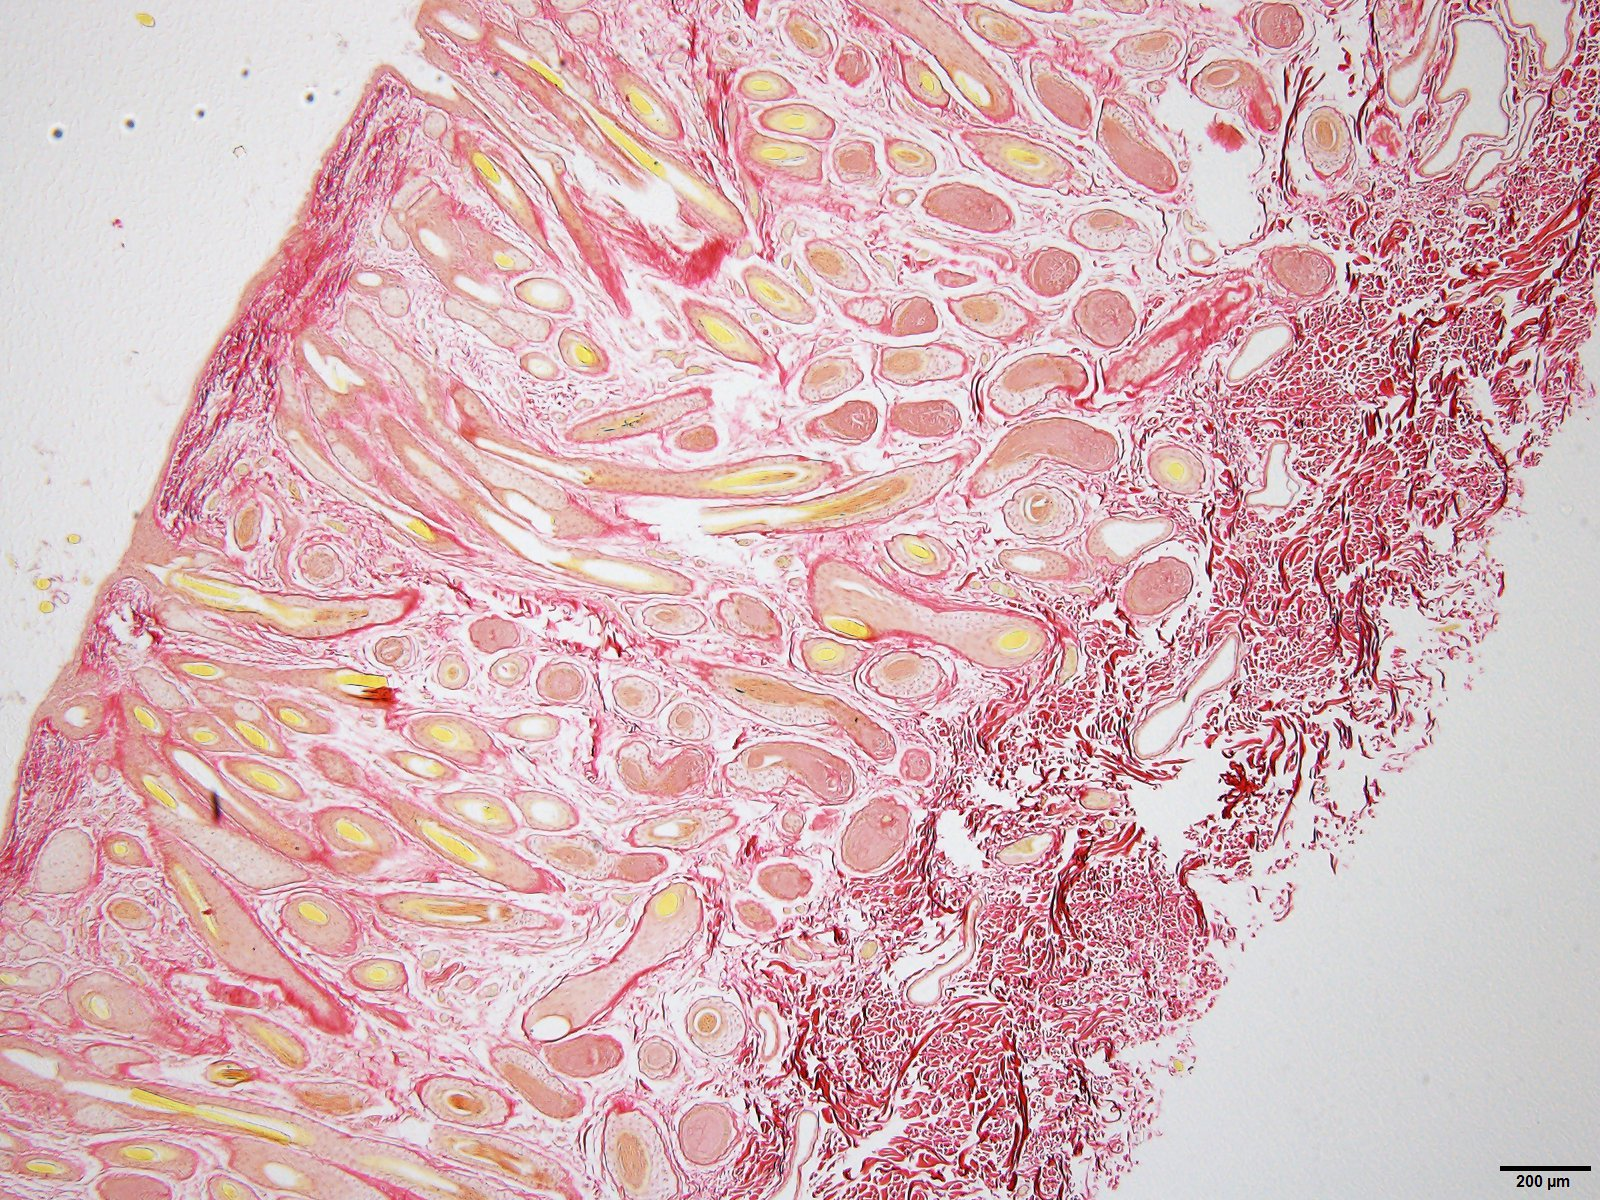
\includegraphics[width=1.0\textwidth]{w479-2-rigid.jpg}
  }
 \subfigure[Sheep 3458 Wrinkle-free]{
%    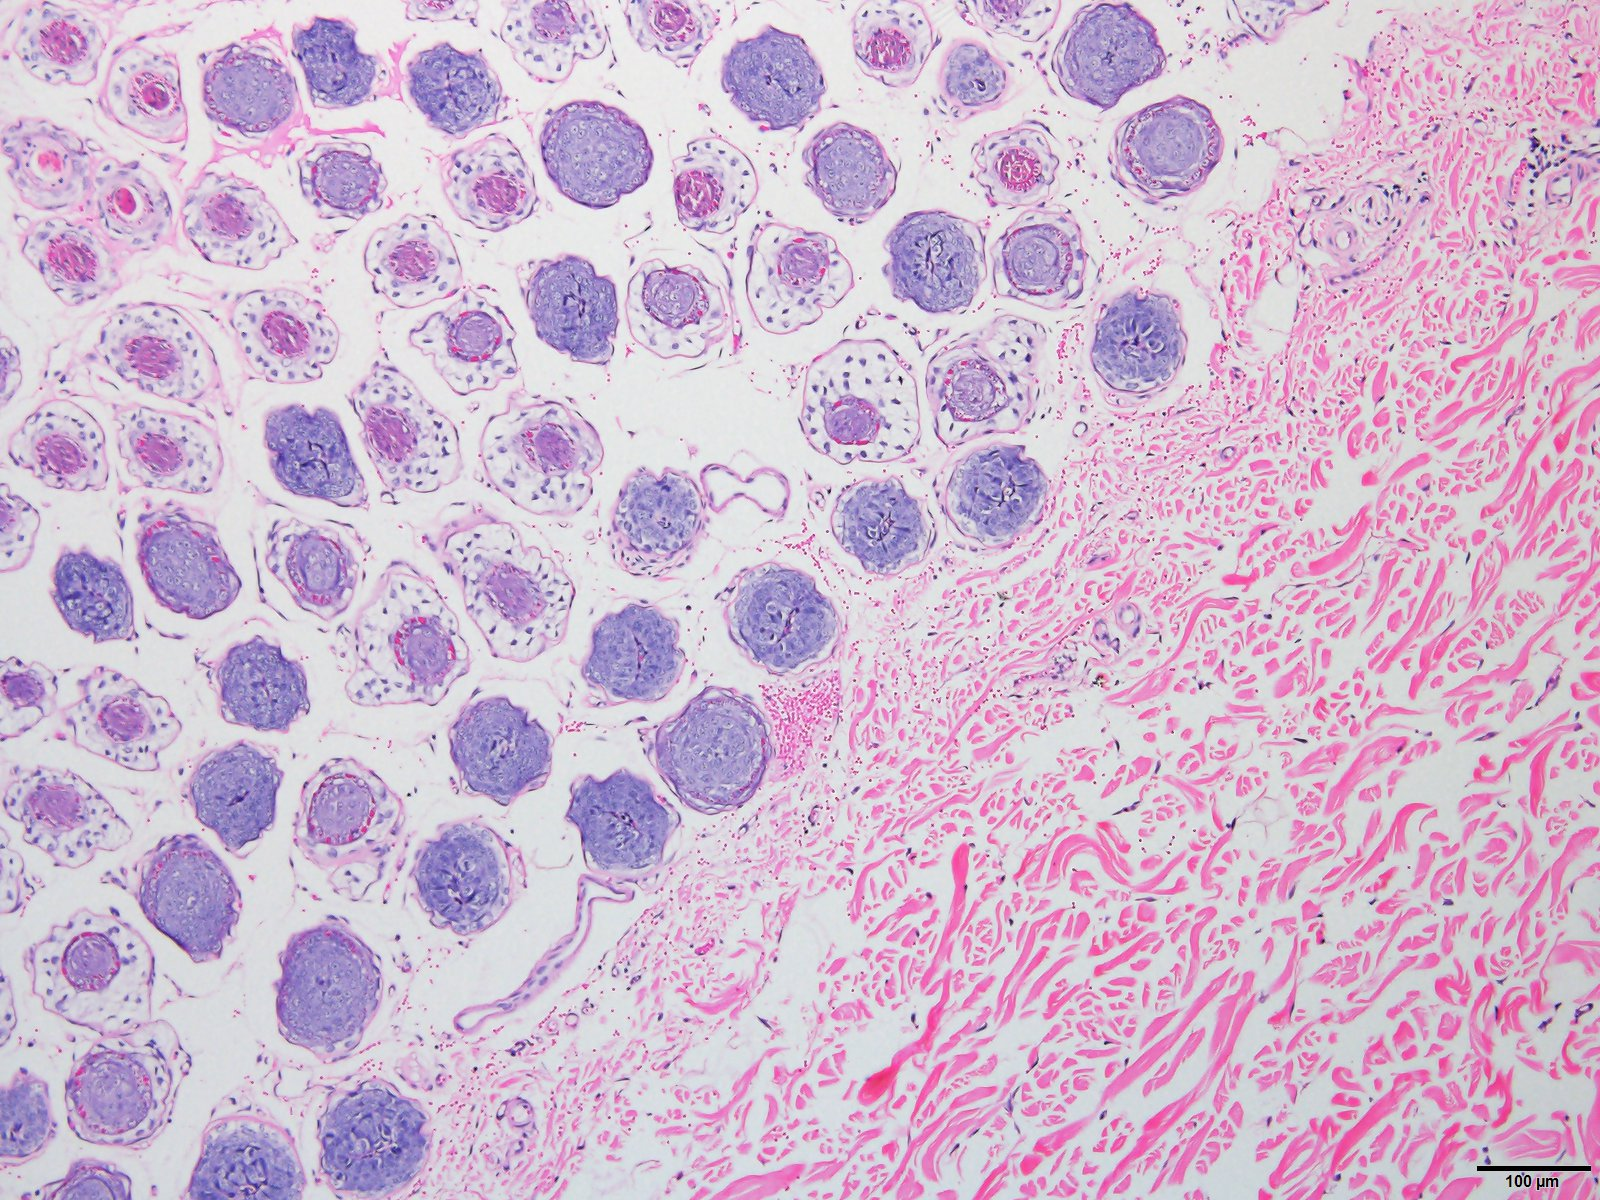
\includegraphics[scale=0.20]{3458_smooth_10x.jpg}
%   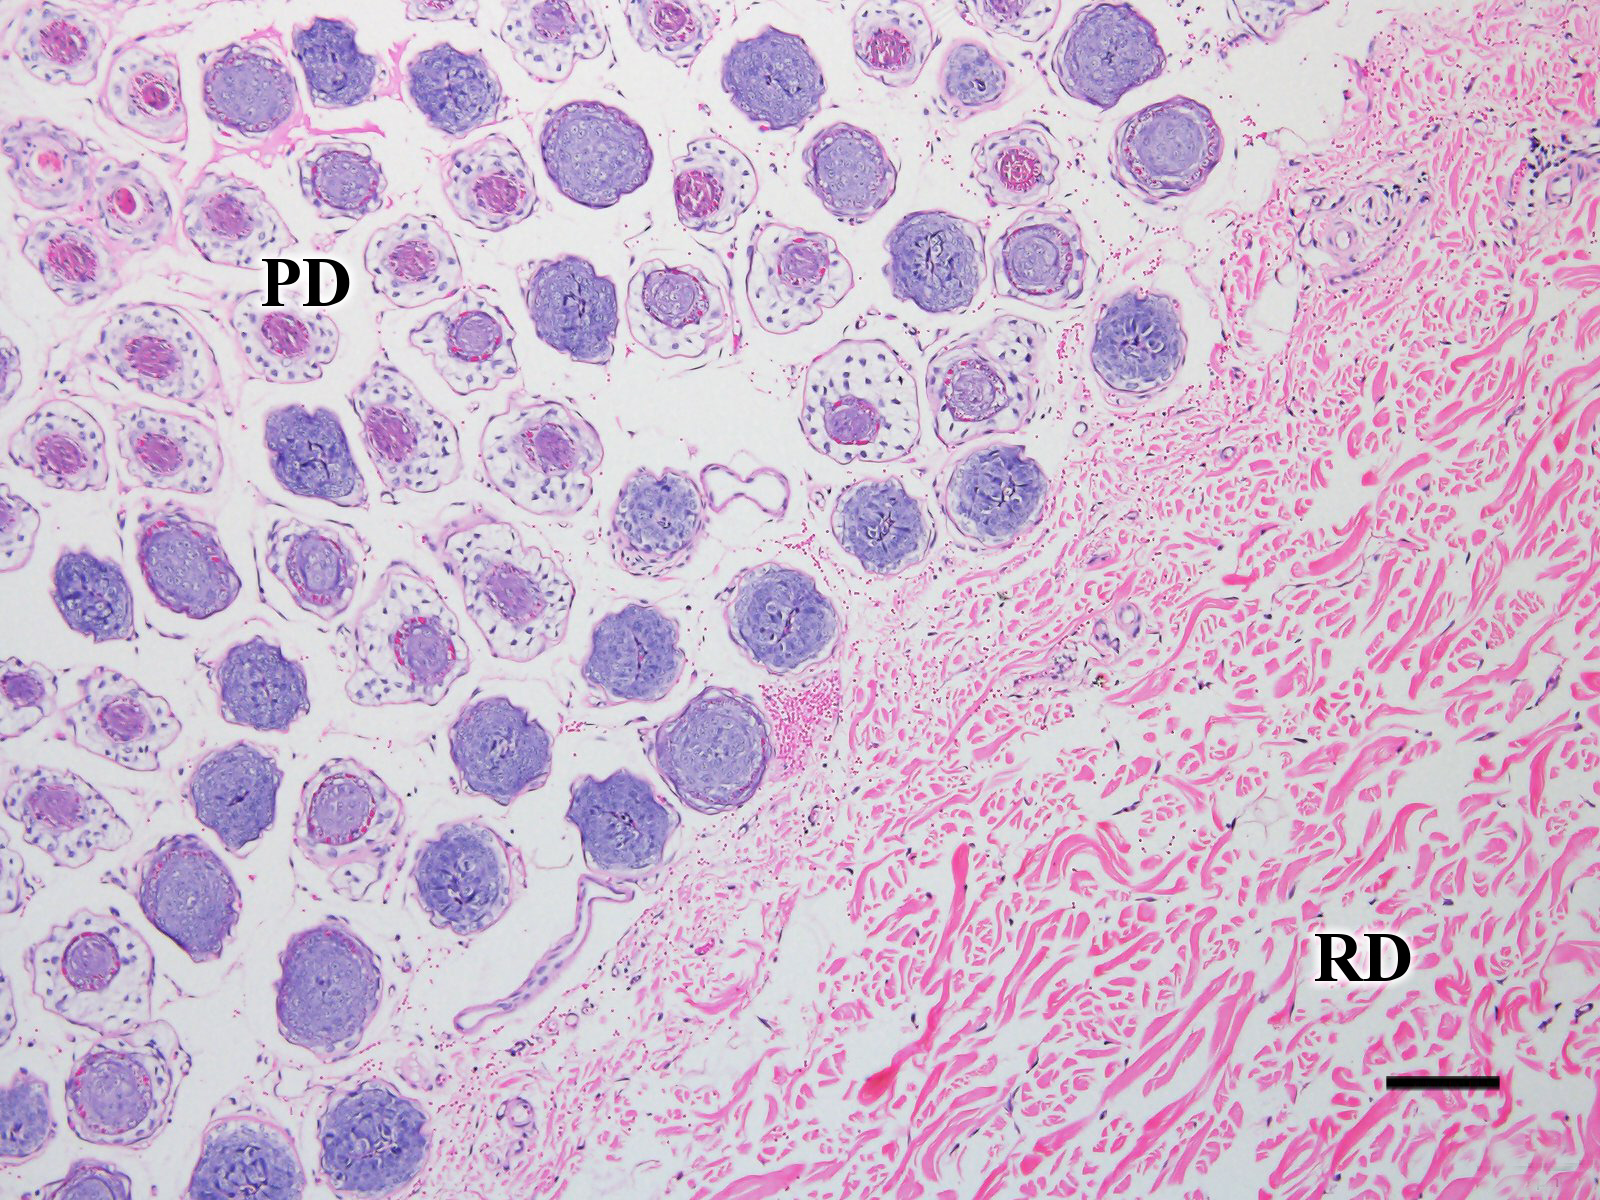
\includegraphics[scale=0.10]{fig8b.jpg}
    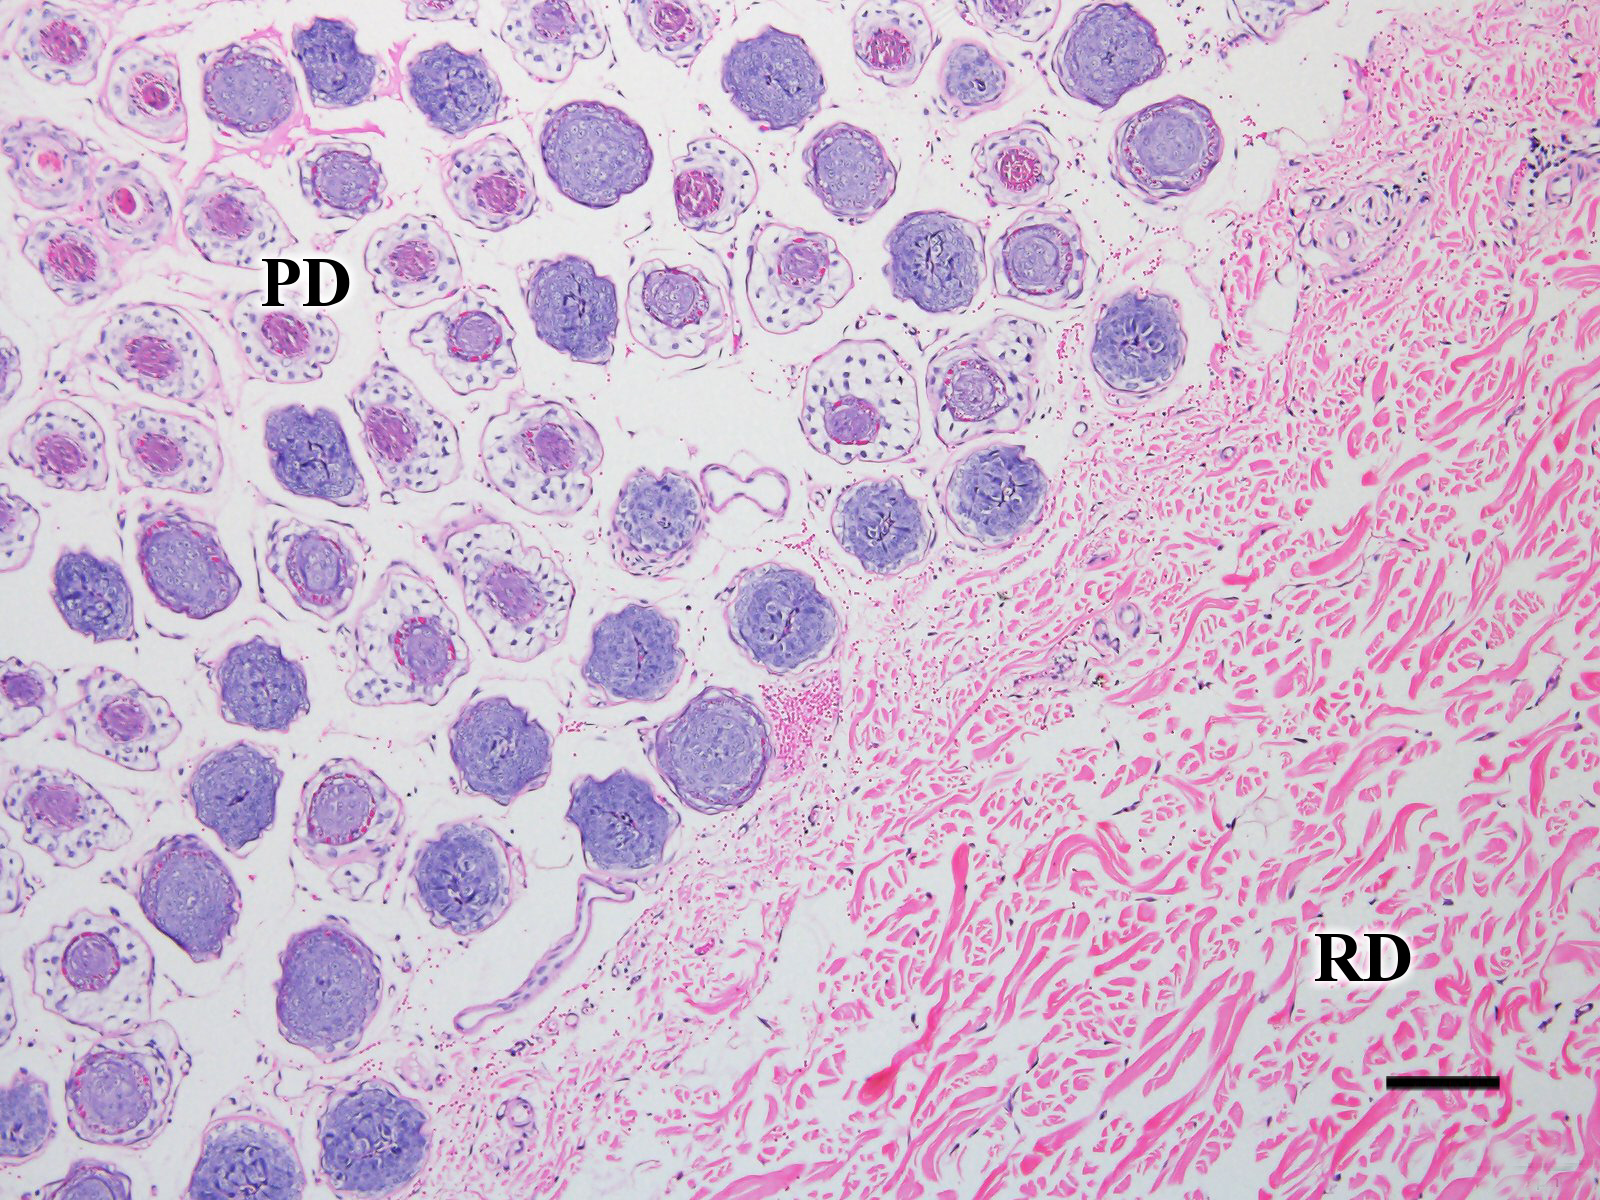
\includegraphics[width=0.7\textwidth]{fig8b.jpg}
  }
  \caption{Vertical sections from a wrinkled (a) and a wrinkle-free (b)  sheep from Trial 2 flock 1 stained with H-E, and viewed with a 10x objective. Skin layers are: {\bf PD} papillary dermis, and {\bf RD} reticular dermis. Scale bar is $80\mu m$.}
\vfill
  \label{fig:he10x}
\end{figure}

%\end{document}


In the wrinkled sheep specimen collagen extends up into the follicular region, there being conspicuous amounts of collagen in and around follicle bulbs. In the wrinkle-free sheep there is little collagen in amongst follicle bulbs, and the collagen immediately below the bulbs is less dense.

Structure also differed. In wrinkled sheep  (Figure~\ref{fig:he10x}a) large pieces of very dense collagen (judging by intensity of staining) occur  in the lower dermis, and amongst the follicles. These are presumably bundles of collagen fibrils. In wrinkle-free sheep (Figure~\ref{fig:he10x}b) the collagen has a more layered appearance, and is almost completely absent from around follicle bulbs.
 These observations are consistent with the PSR stained images of Figure~\ref{fig:psr40x}. The bundles of collagen which show as large continuous areas in these sections are aligned with the direction of sectioning. Fibre bundles that have been sectioned across appear as smaller entities. There are fewer large entities in the wrinkle-free specimens in both Figures~\ref{fig:psr40x} and ~\ref{fig:he10x}. This difference is also discernible in Figure~\ref{fig:trial24xhe}


\subsubsection{Type of collagen}

One can distinguish Type  I and II  collagen from size of the bundles of fibrils. For example in  the PSR stained images of Figure~\ref{fig:psr40x} the wrinkled specimen clearly has large bundles of fibrils and therefore a considerable amount of Type I collagen. The wrinkle-free specimen, however has fewer bundled fibrils, and therefore a lesser amount of Type I collagen, as seen in Figures~\ref{fig:he10x} and ~\ref{fig:trial24xhe}.

A  technique referred to in Section~\ref{sec:matmeth}, which uses polarised light microscopy was used  to differentiate Type I from Type III collagen.  
Figure~\ref{fig:polar} shows two polarised light images under a 4x objective comparing a wrinkled sheep with a wrinkle-free sheep.
%\documentclass{article}
%\usepackage{graphicx,subfigure}
%\usepackage{caption,rotating}
%\begin{document}

\begin{figure}[!h]
\centering
\captionsetup{width=0.92\textwidth}
 \subfigure[Sheep w479 Wrinkled]{
%    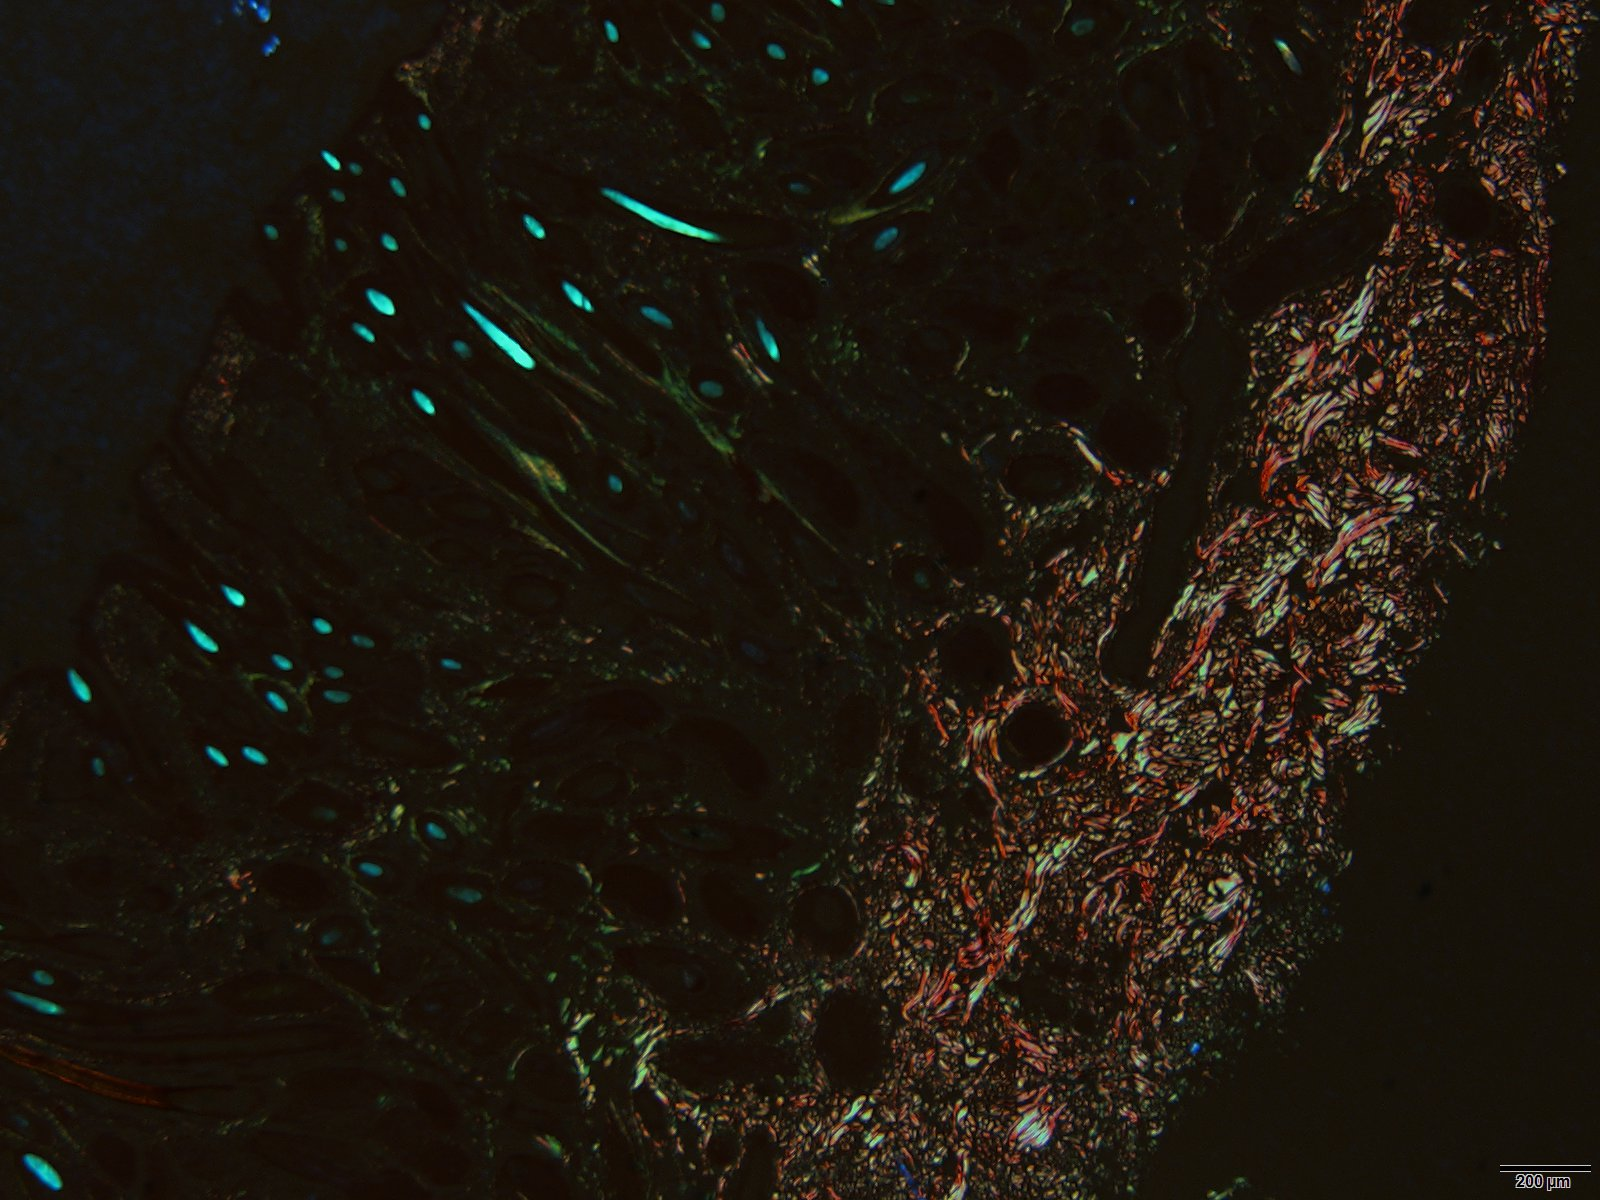
\includegraphics[scale=0.20]{w479-2_rigid_PSR_stain_polarised.jpg}
%   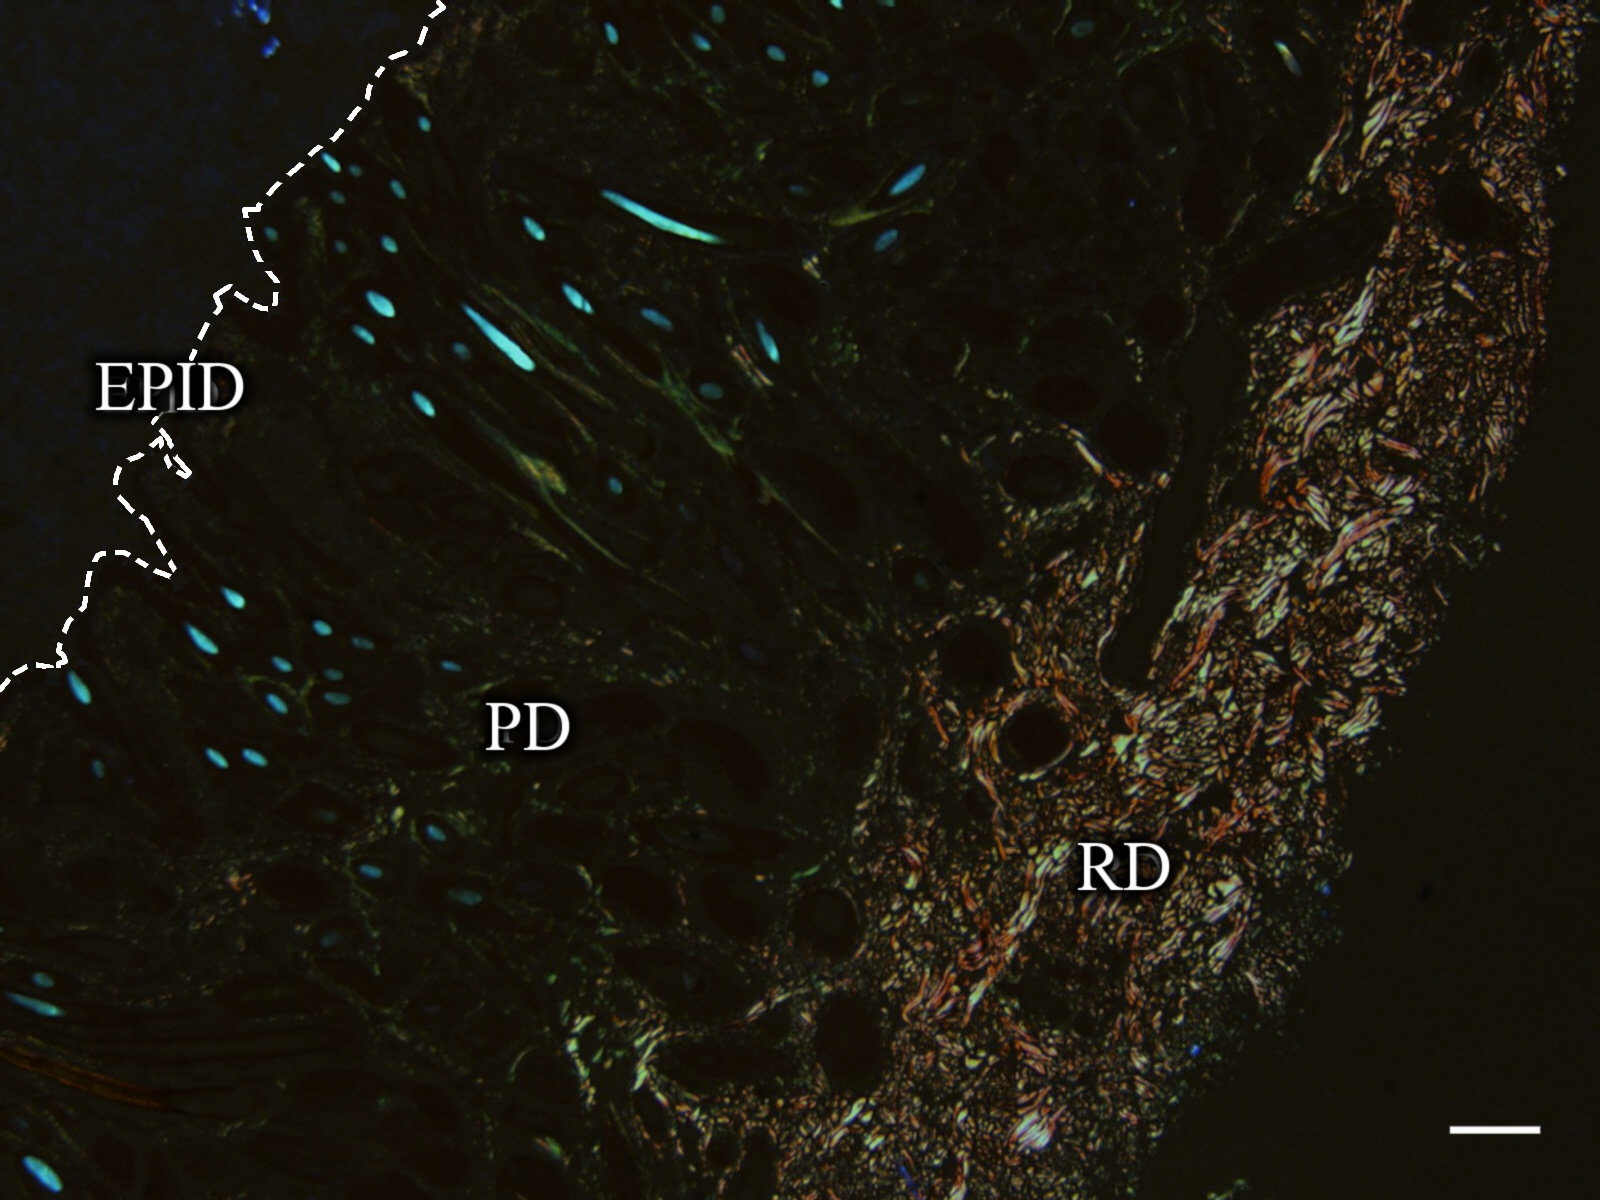
\includegraphics[scale=0.10]{fig9a.jpg}
    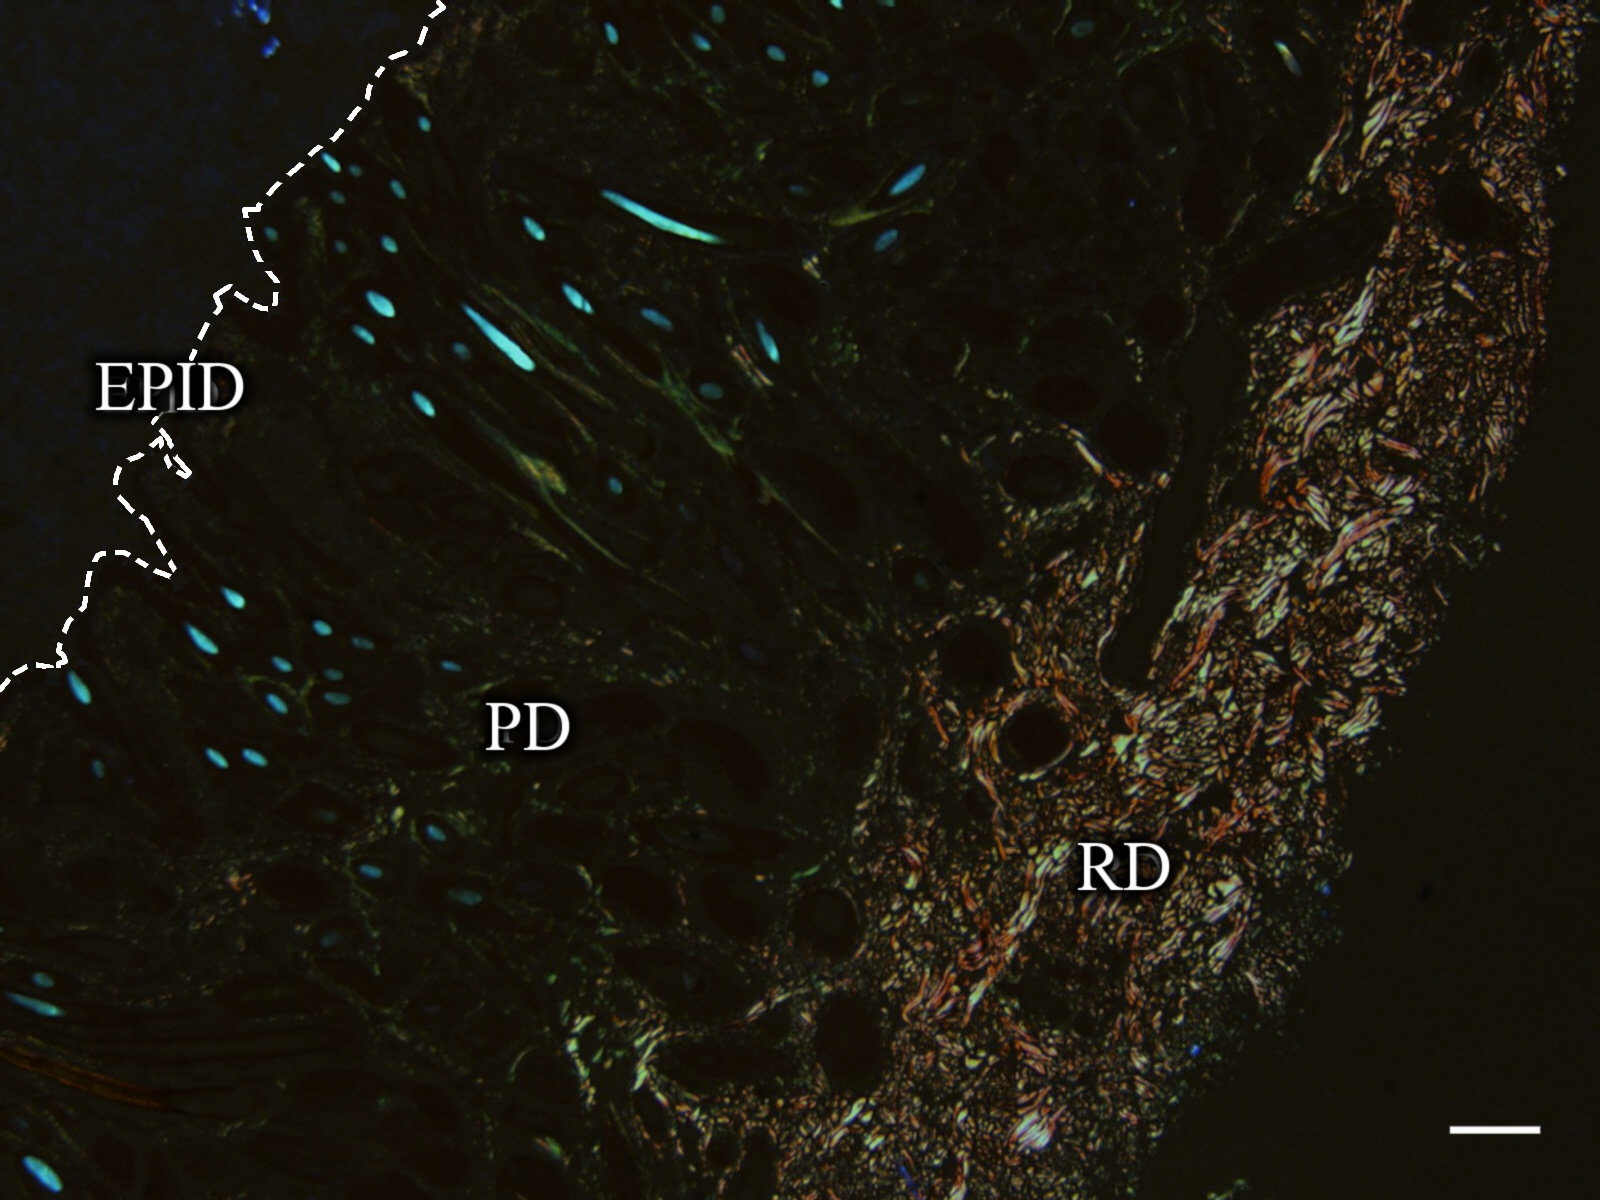
\includegraphics[width=0.45\textwidth]{fig9a.jpg}
% 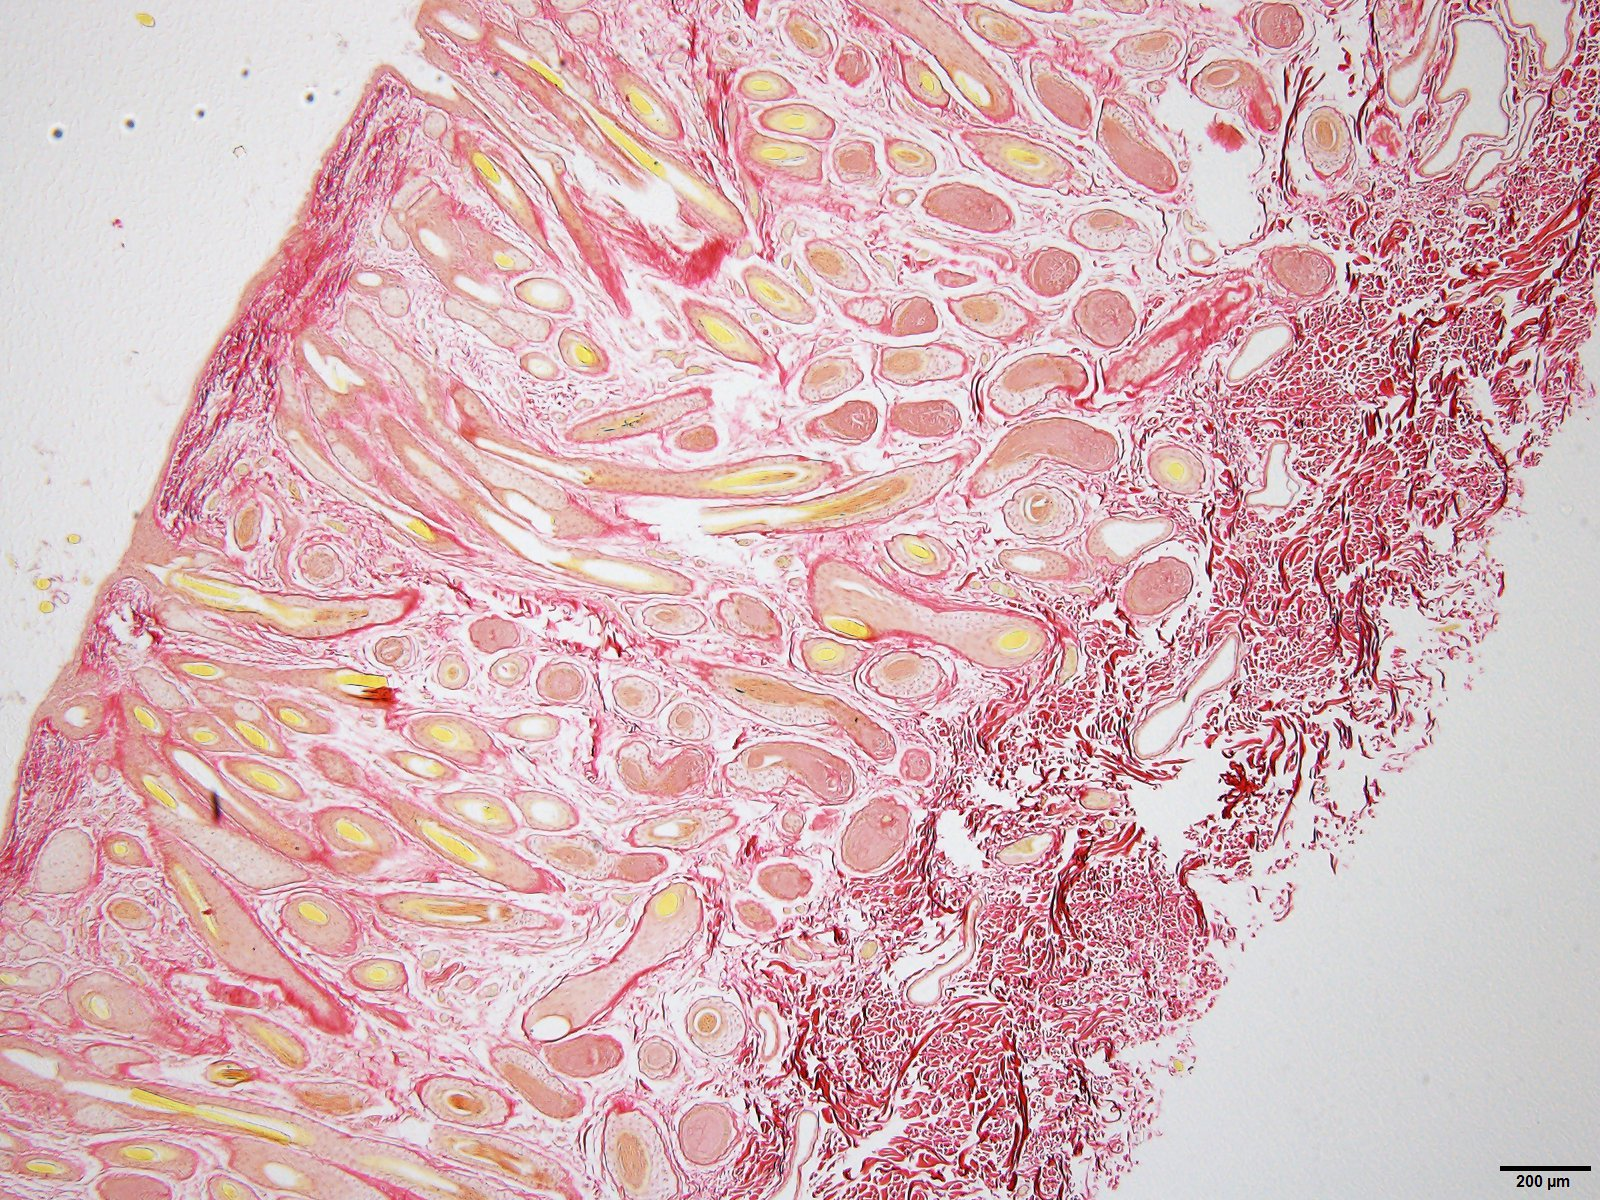
\includegraphics[width=1.0\textwidth]{w479-2-rigid.jpg}
  }
 \subfigure[Sheep w490 Wrinkle-free]{
%    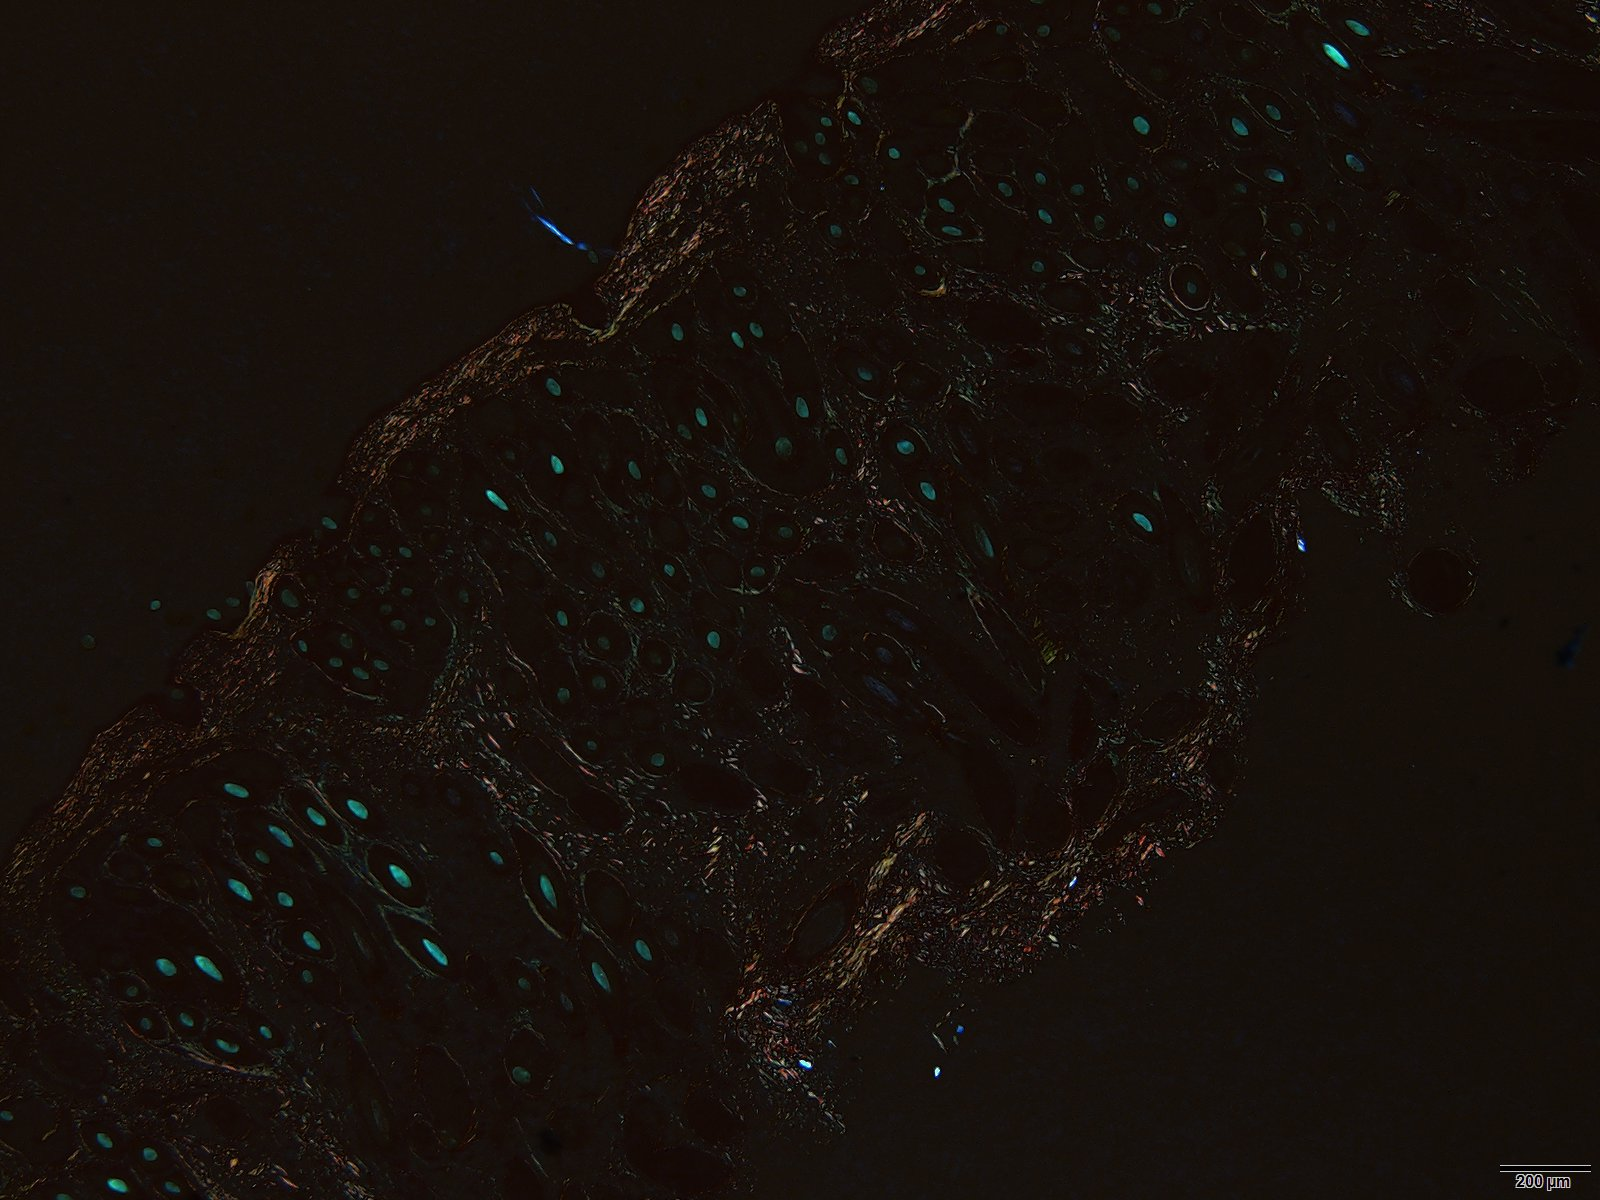
\includegraphics[scale=0.20]{w490-2_supple_PSR_stain_polarised.jpg}
%   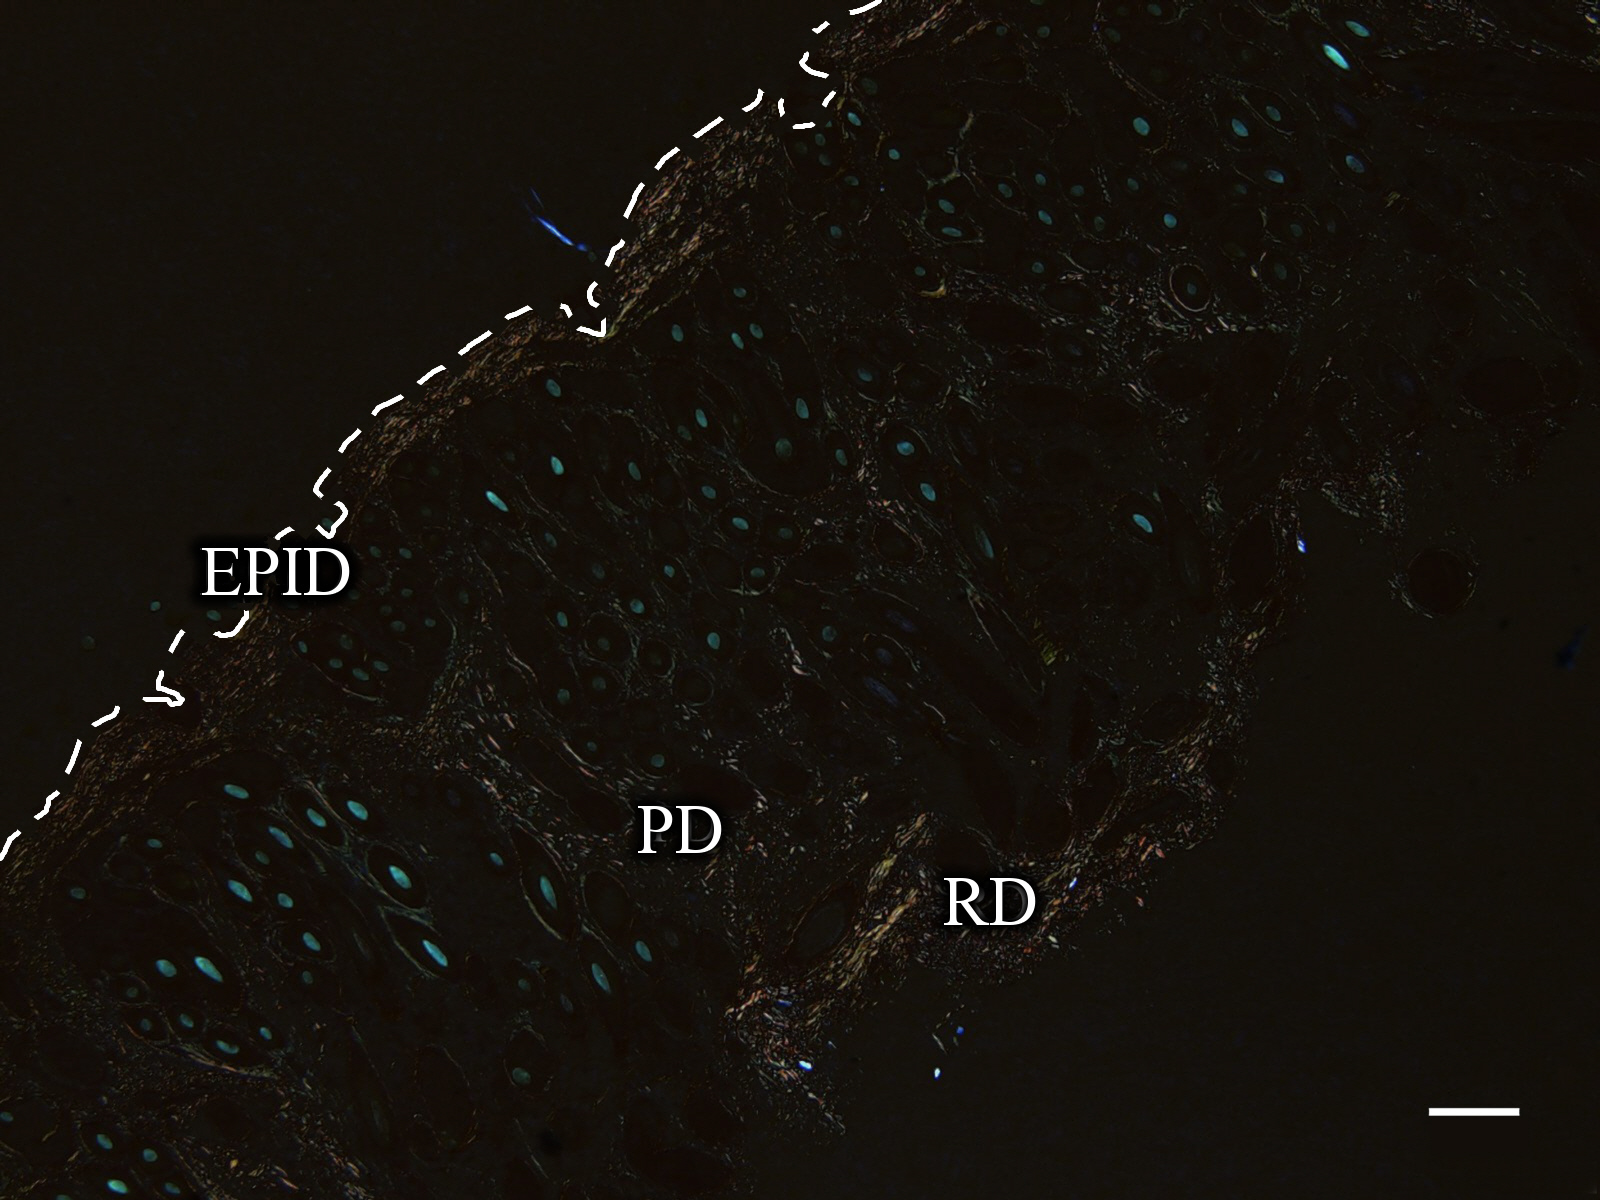
\includegraphics[scale=0.10]{fig9b.jpg}
    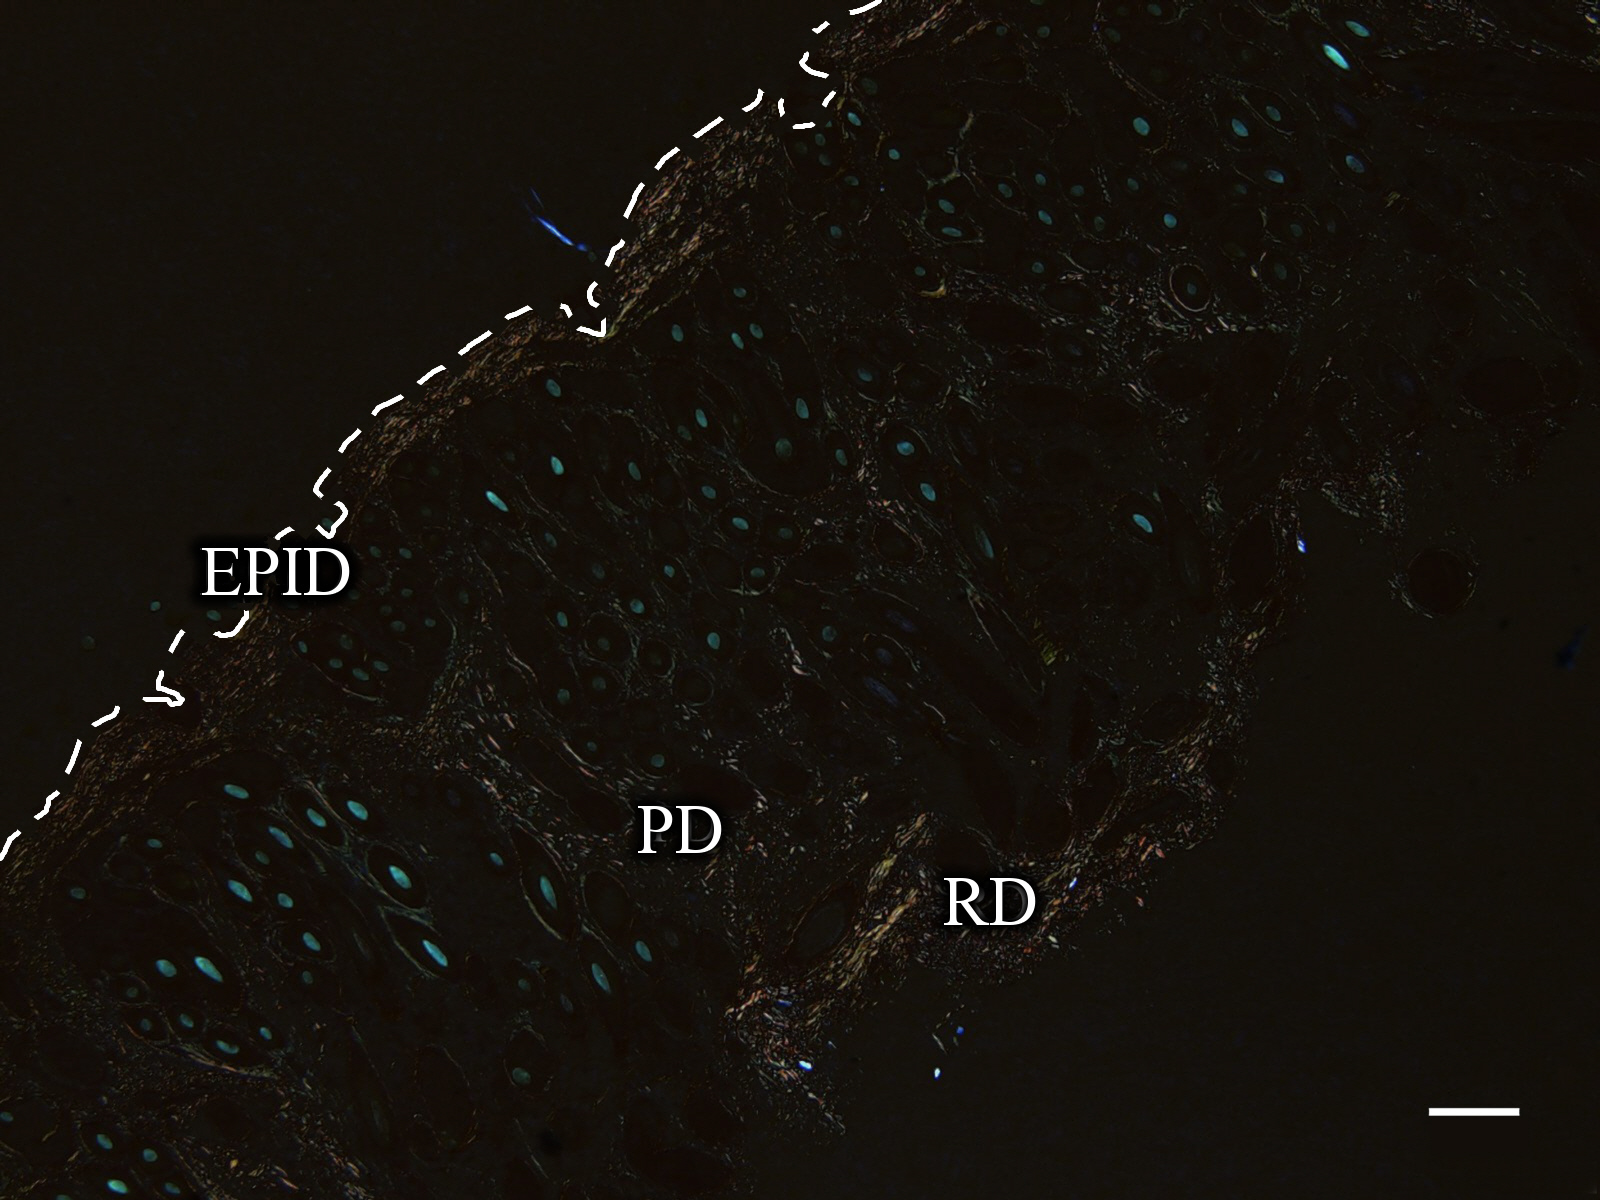
\includegraphics[width=0.45\textwidth]{fig9b.jpg}
  }
  \caption{Vertical sections from a wrinkled (a) and a wrinkle-free (b) sheep from Trial 1 flock 2 stained with PSR and examined with polarised light and a 4x objective. Skin layers are: {\bf EPID} epidermis, {\bf PD} papillary dermis, and {\bf RD} reticular dermis. Epidermal surface is marked with a dotted line. Scale bar is $200\mu m$. }
\vfill
  \label{fig:polar}
\end{figure}

%\end{document}


The same sections viewed under bright field microscopy are shown in Figure~\ref{fig:nopolar}. 
%\documentclass{article}
%\usepackage{graphicx,subfigure}
%\usepackage{caption,rotating}
%\begin{document}

\begin{figure}[!h]
\centering
\captionsetup{width=0.92\textwidth}
 \subfigure[Sheep w479 Wrinkled]{
%    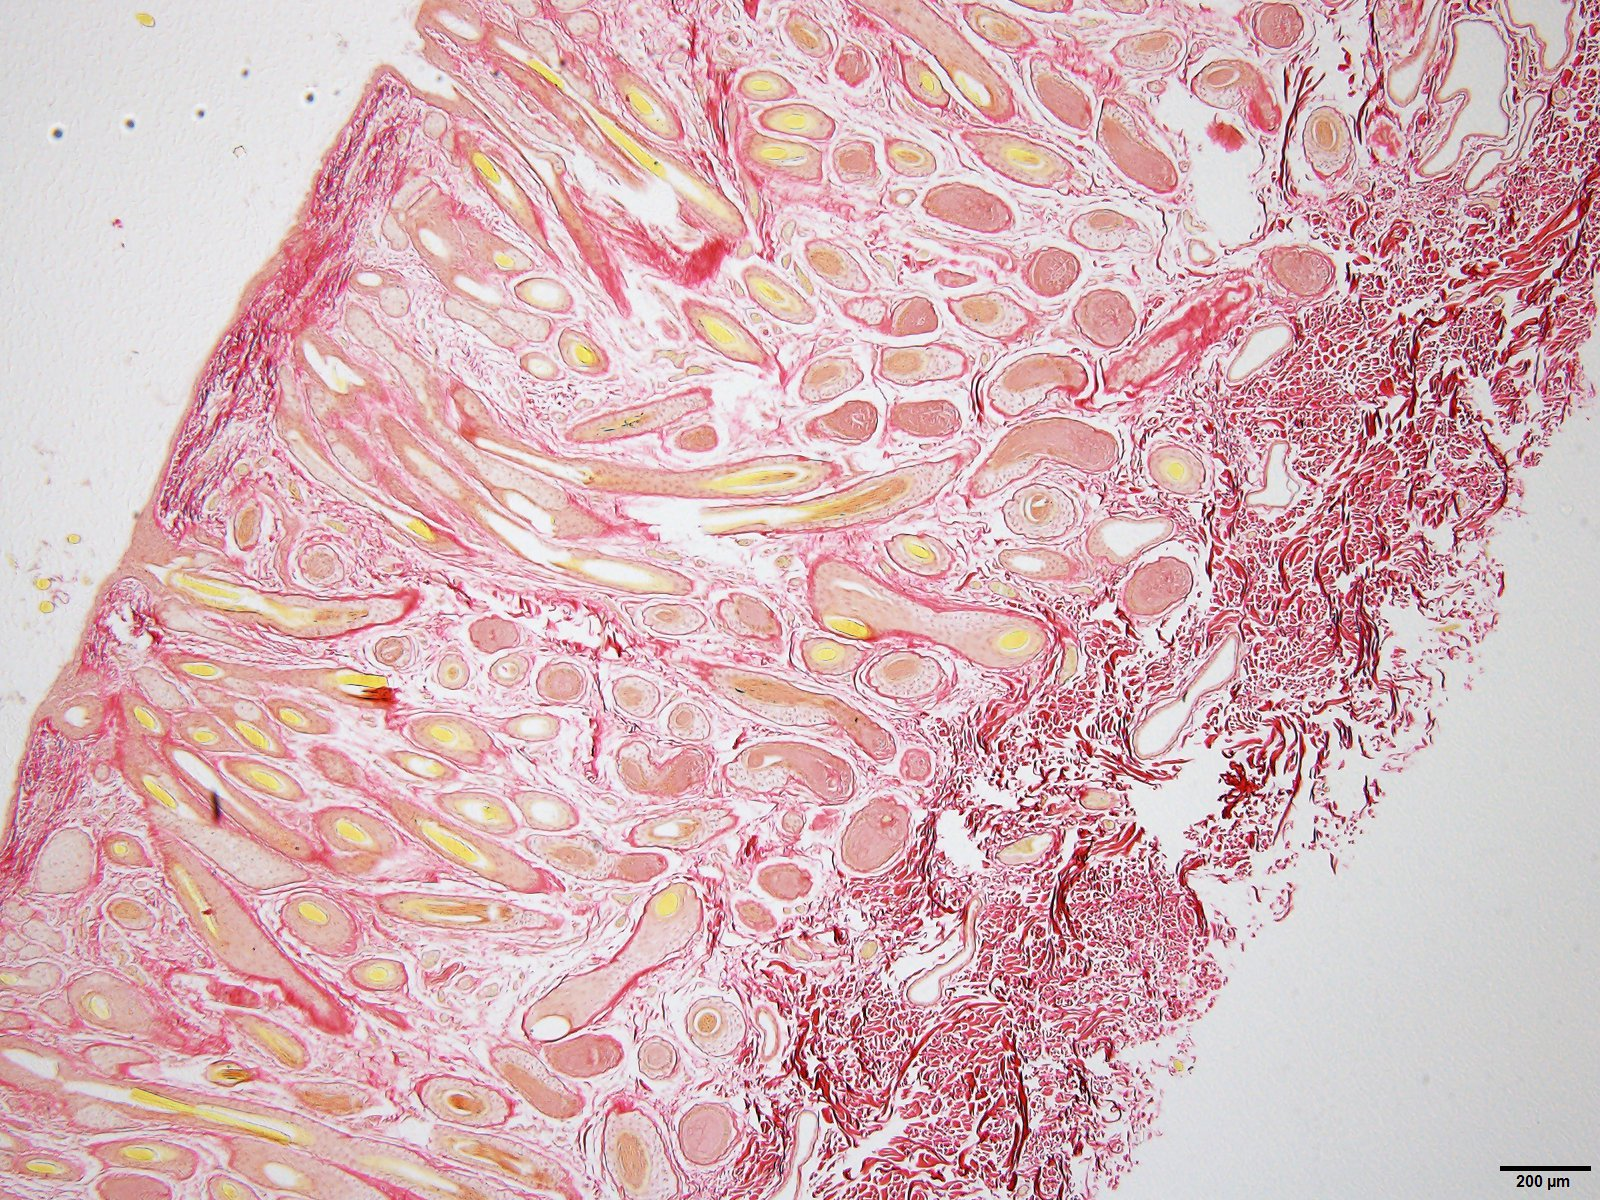
\includegraphics[scale=0.20]{w479-2-rigid.jpg}
%   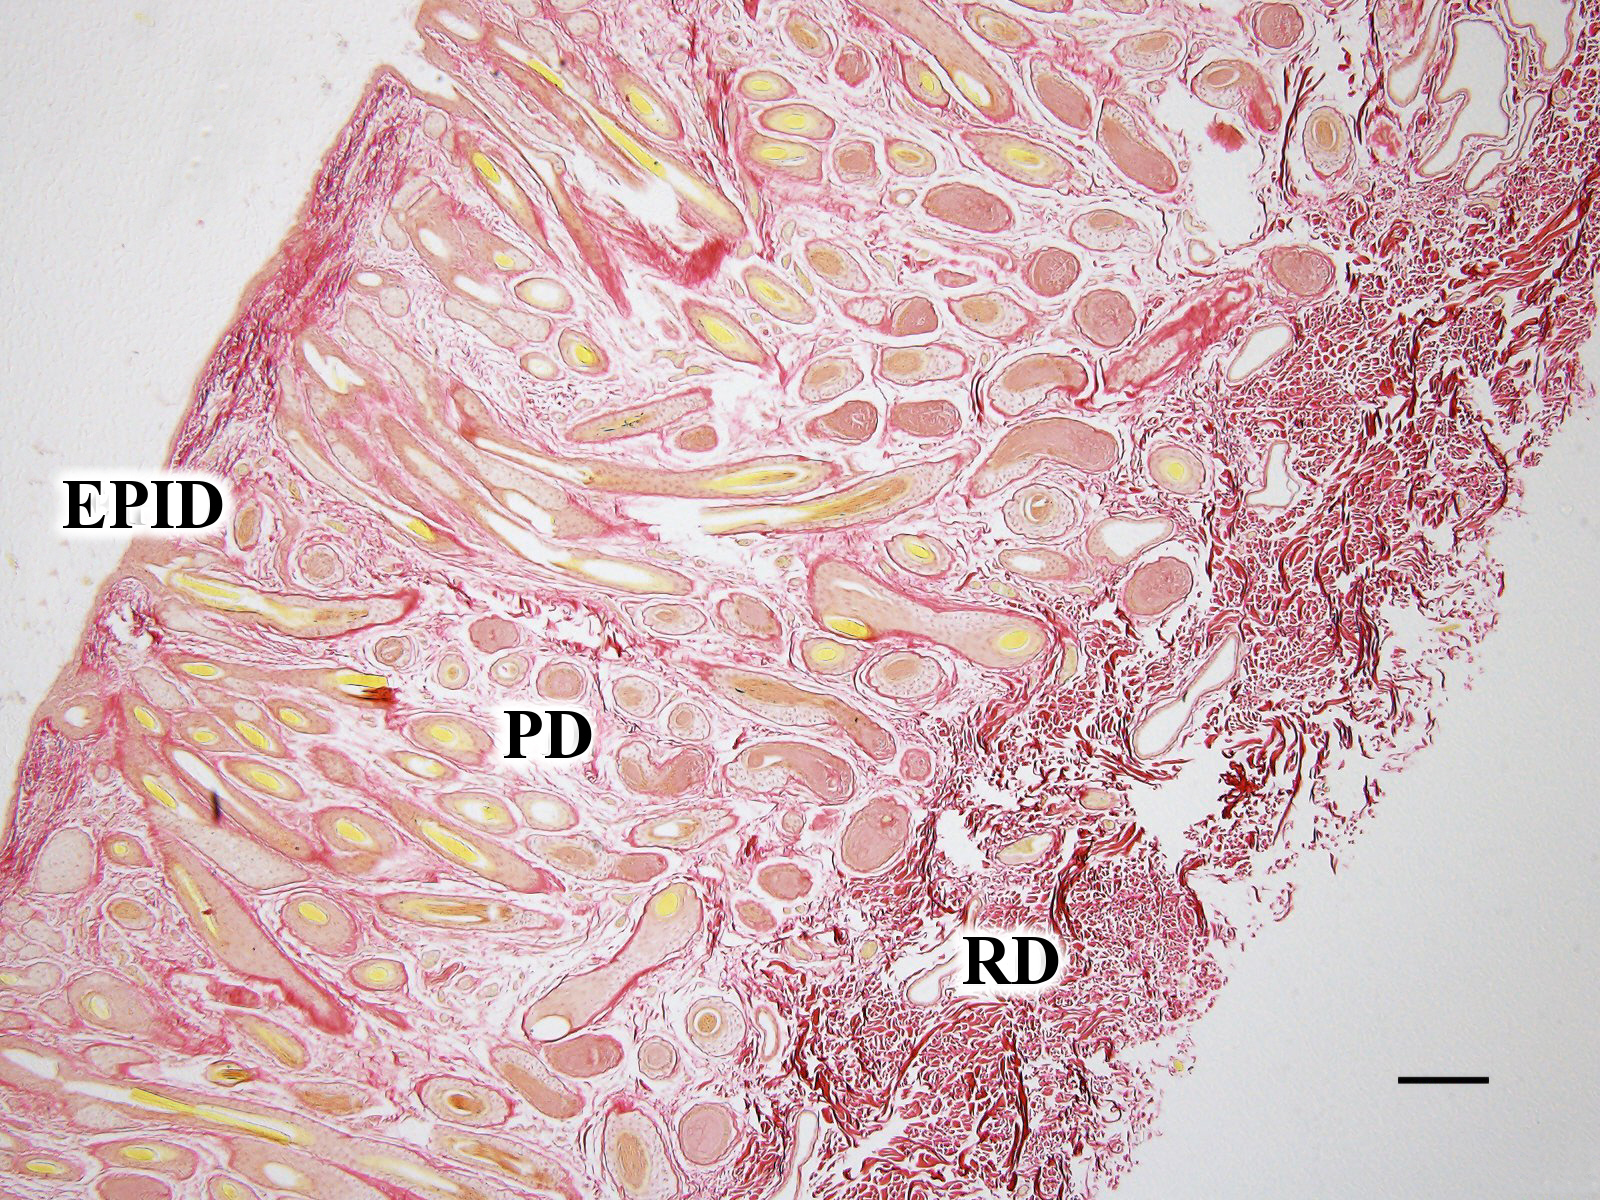
\includegraphics[scale=0.10]{fig10a.jpg}
    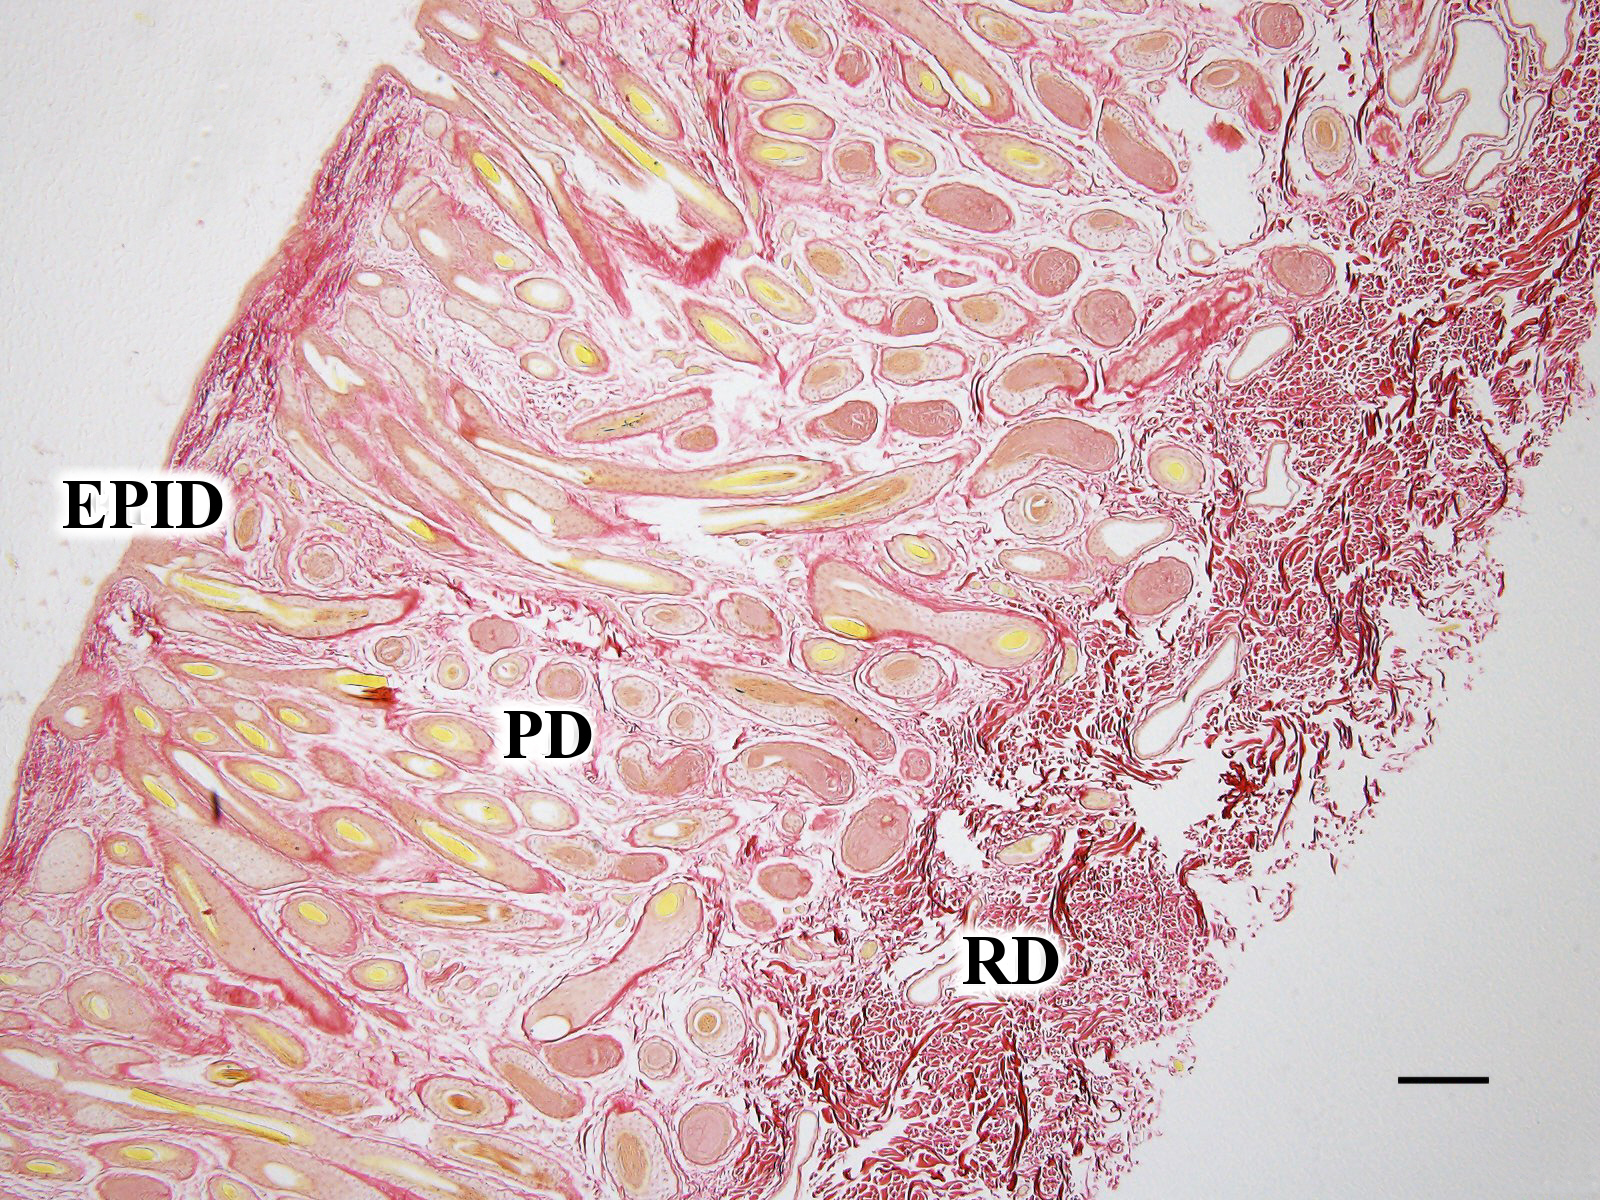
\includegraphics[width=0.45\textwidth]{fig10a.jpg}
  }
 \subfigure[Sheep w490 Wrinkle-free]{
%    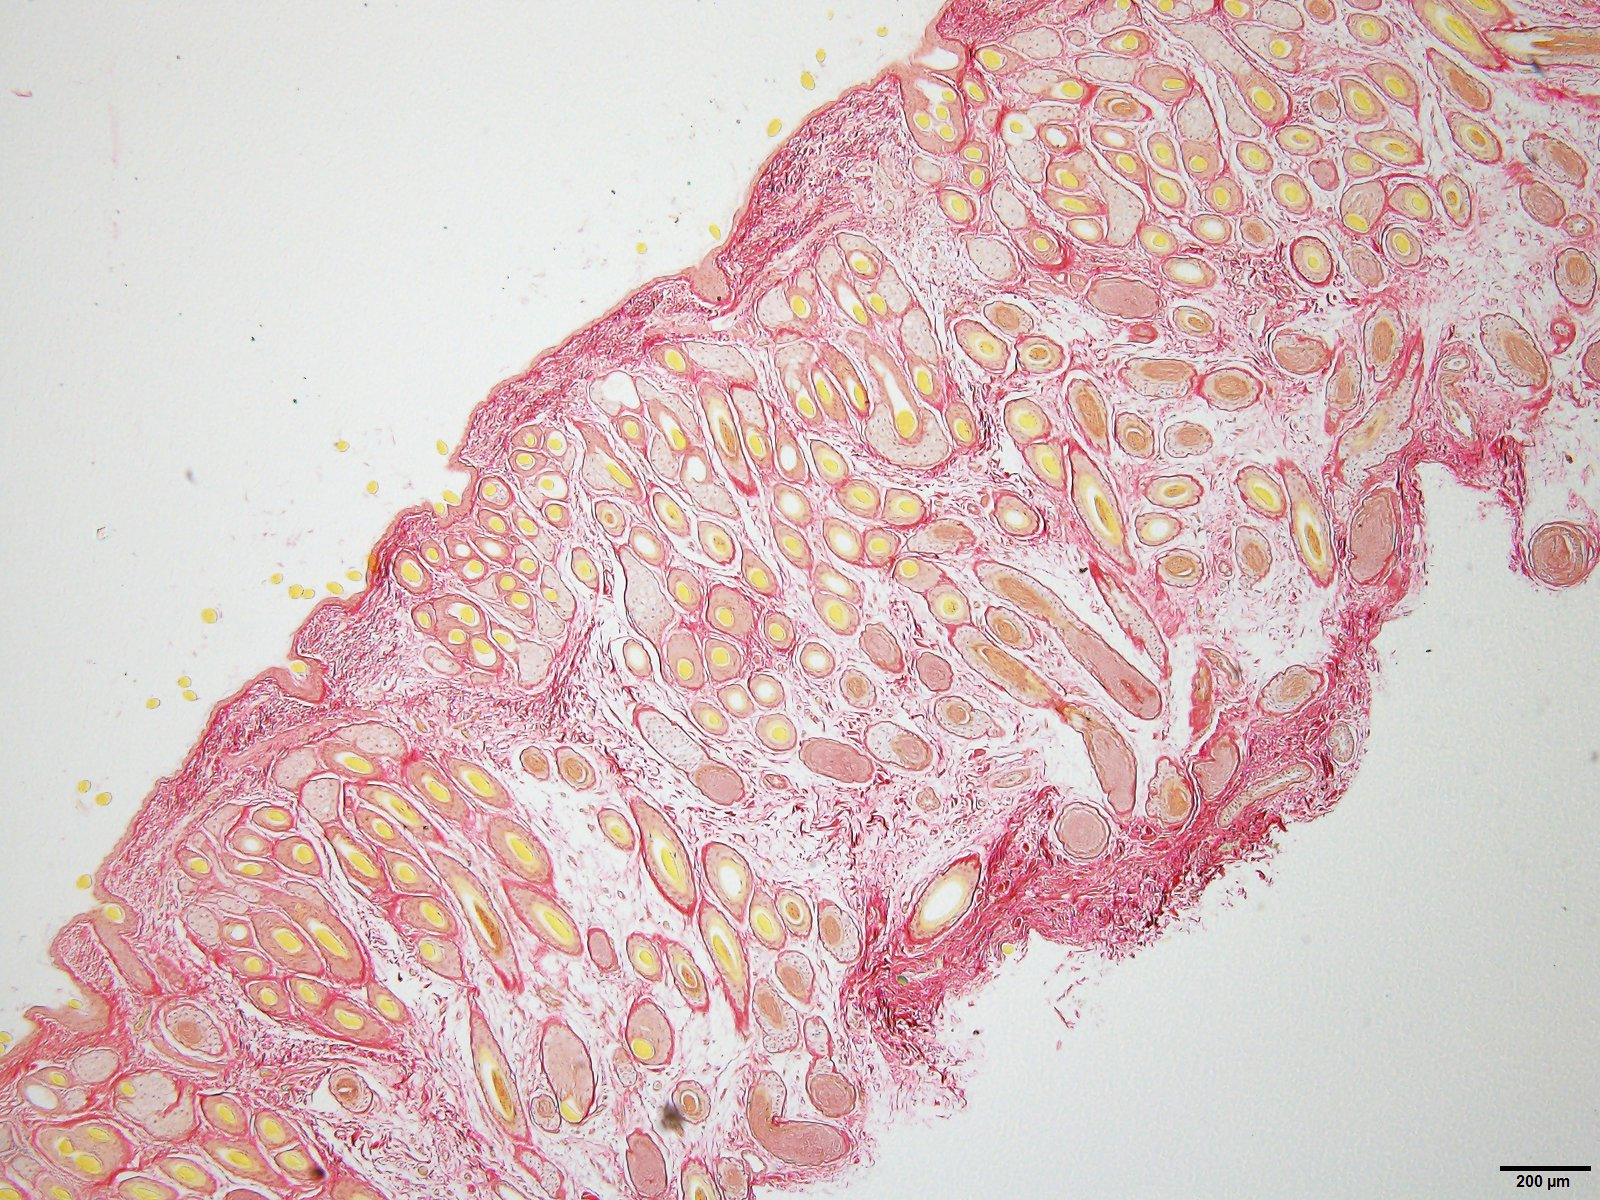
\includegraphics[scale=0.20]{w490-2-supple.jpg}
%   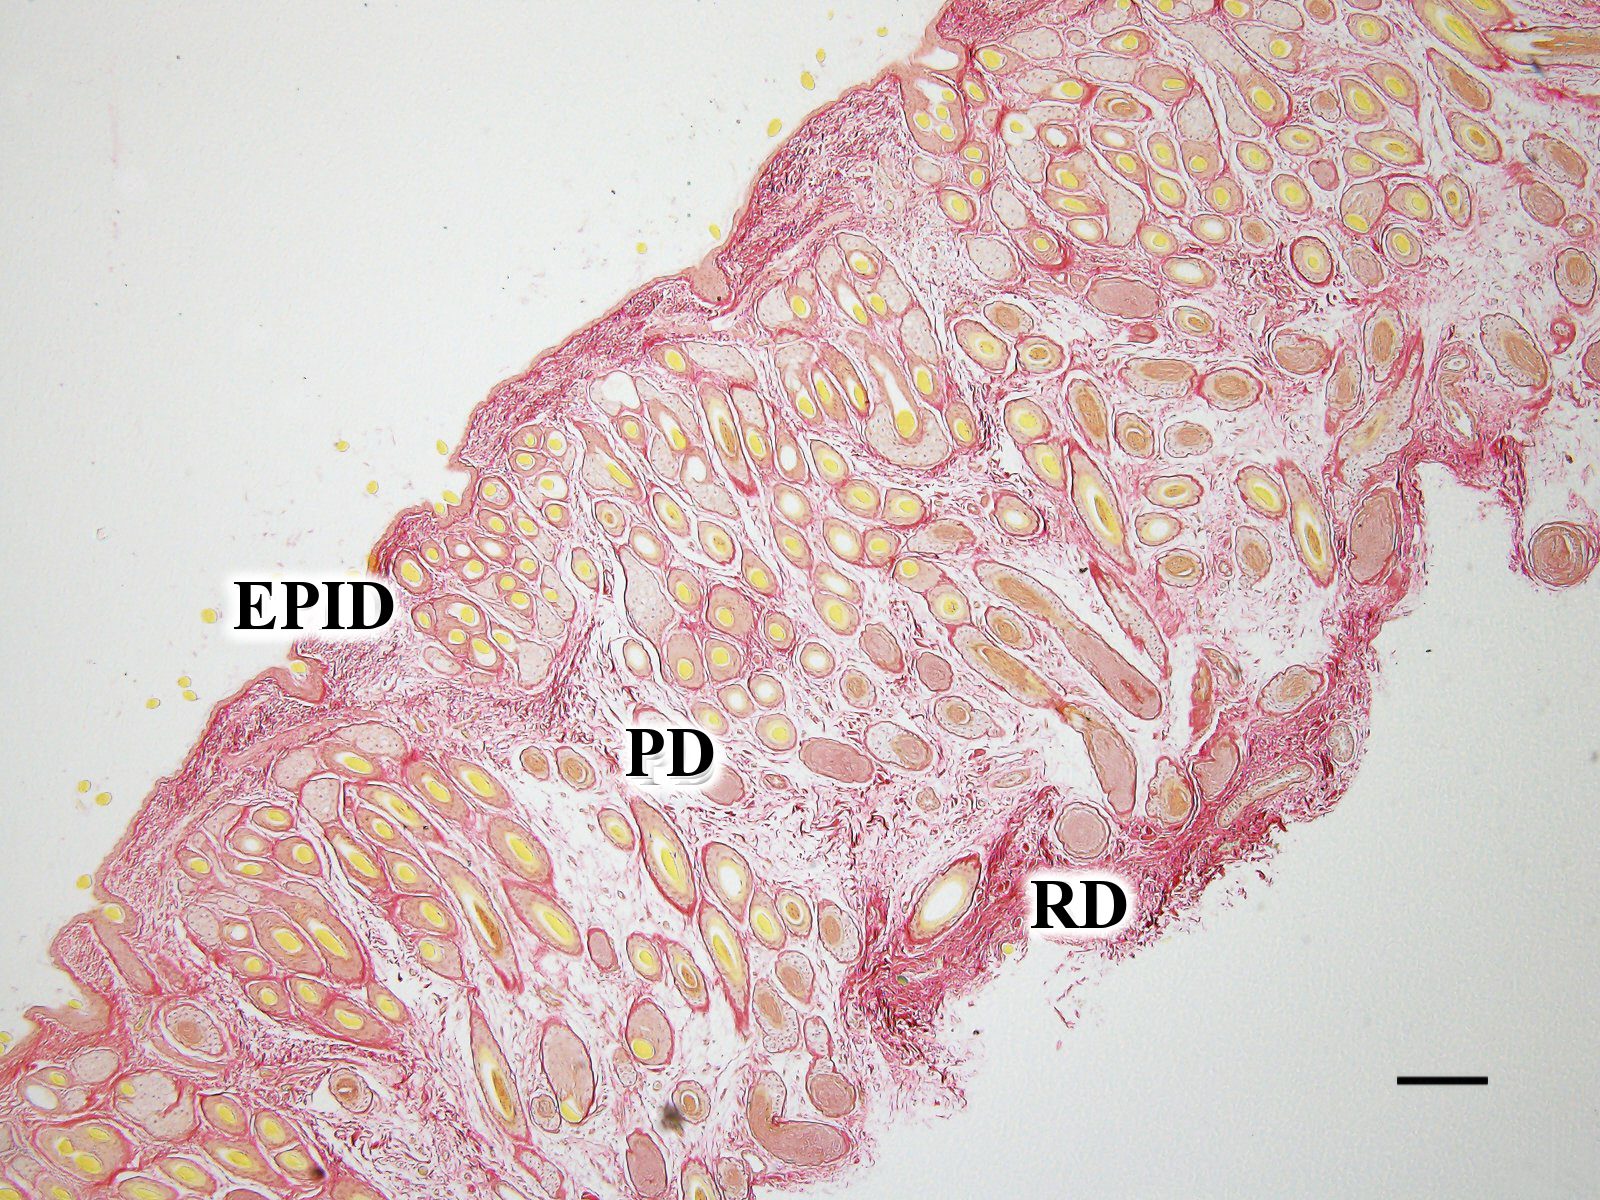
\includegraphics[scale=0.10]{fig10b.jpg}
    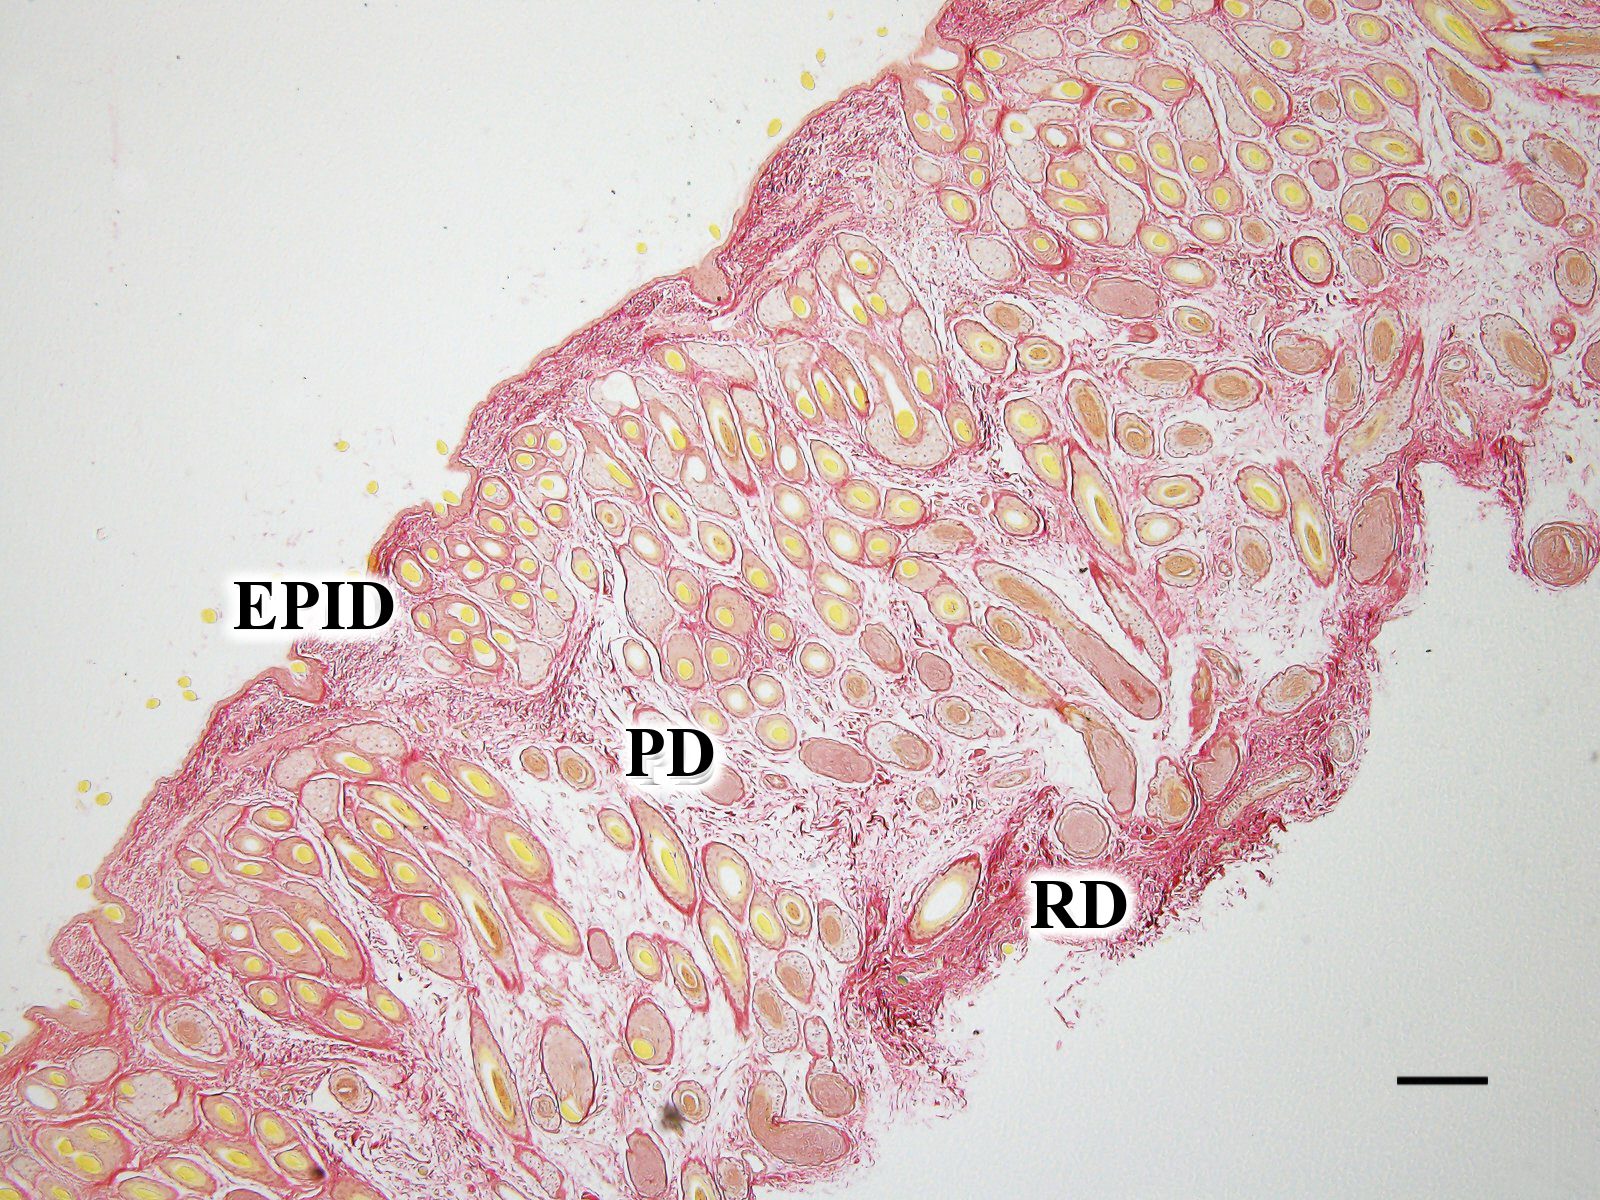
\includegraphics[width=0.45\textwidth]{fig10b.jpg}
  }
  \caption{Vertical sections from a wrinkled (a) and a wrinkle-free (b) sheep from Trial 1 flock 2 stained with PSR and examined with a 4x objective. These are the same two sections as shown with polarised light in Figure~\ref{fig:polar}. Skin layers are: {\bf EPID} epidermis, {\bf PD} papillary dermis, and {\bf RD} reticular dermis. Scale bar is $200\mu m$. }
\vfill
  \label{fig:nopolar}
\end{figure}

%\end{document}



Both wrinkled and wrinkle-free specimens have some lower dermal collagen (stained red with PSR stain in Figure~\ref{fig:nopolar}), but only the wrinkled specimen shows orange/red birefringence under polarised light (Figure~\ref{fig:polar}).  Because these specimens are from Trial 1, it is possible that some of the lower dermis was removed in trimming the biopsy specimens. This should not affect comparison of collagen types.

 It is evident that wrinkled sheep do not just have more collagen, but the extra collagen is Type I (hard). Wrinkle-free sheep apparently only have Type III (reticular) collagen. This confirms the conclusion of the previous section from looking at size of collagen fibre bundles.

\subsection{Wrinkle patterns over body}
\label{sec:pattern}
All Merinos have small {\em pin} wrinkles. Pin wrinkles do not seem to form a pattern and are uniform across the body. Here, patterns in the large wrinkles which develop from birth up to maturity, are discussed. Large wrinkles form a consistent pattern which was documented by \citep{carter-1943}. \citeauthor{carter-1943} named each wrinkle and associated them with successive vertebrae along the spine. Size of wrinkles varies, but not the pattern. The pattern is consistent between sheep.  Figure~\ref{fig:sheep} shows a photograph of two Merino ewes, with and without wrinkle. 
%\documentclass{article}
%\usepackage{graphicx,subfigure}
%\begin{document}

\begin{figure}[!h]
  \centering
 \captionsetup{width=0.7\textwidth}
  \includegraphics[width=0.7\textwidth,angle=180]{IMG_0322.JPG}
  \caption{Two Merino ewes from Flock 1 of Trial 2, one wrinkled (left) and one wrinkle-free (right)}
  \label{fig:sheep}
\end{figure}

%\end{document}


The wrinkled sheep in Figure~\ref{fig:sheep} is a good example of the pattern to which we refer.  Each wrinkle runs dorso-ventrally, the numbers of wrinkles approximating those of the vertebrae. Each wrinkle appears to mark the position one {\em dermatome} area of skin \citep{kirk-1968}, with the main nerve from the spine running either under or between wrinkles. We do not know the spatial relationship between wrinkles and nerve channels but is appears to be a one-to-one relation.

Wrinkles on the side of a sheep run vertically. Rows of follicle groups on the side of a sheep run vertically. In mosaic sheep \citep{fraser-1960}, which are somatic fleece mutations, the patterns of mutant fleece run vertically.  These phenomena reflect the way skin develops, as a series of separate patches called dermatomes, each patch being associated with one nerve descending from the spine. The reason wrinkle development follows this pattern remains unexplained.

\section{Discussion}
This study has established from observations on adult Merino sheep that wrinkled sheep have the following:
\small
\begin{itemize}
\item[$-$] more collagen in the lower dermis
\item[$-$] more Type I collagen in the lower dermis
\item[$-$] collagen in the lower dermis extending upwards around follicle bulbs into the upper dermis
\end{itemize}
\normalsize
Comparison of skin from paired sites on the same sheep,  {\em  on-wrinkle} and {\em off-wrinkle}, has shown that there is no difference in collagen Type or amount.
In addition published work has established the following:
\small
\begin{itemize}
\item[$-$] wrinkles have been reported forming in foetal skin of Karakul and Merino lambs at around 100 days of gestation \citep{bogolyubsky-1940}
\item[$-$] pin wrinkles are small and are present at birth and remain into adulthood. Pin wrinkles are mainly a characteristic of Merino sheep \citep{carter-1943}
\item[$-$] wrinkles are visible at birth and grow in size as a sheep matures. They are also mainly a characteristic of some Merino sheep. Wrinkles form in a pattern which suggests a one to one relation between wrinkles and dermatomes \citep{carter-1943}
\item[$-$] large wrinkles consist of epidermis, papillary dermis, and lower or reticular dermis, but not the muscle and fat layers \cite{mitchell-1984}
\item[$-$] collagen is present in the foetal dermis from about day 80, ie at about the same time as when secondary derived follicles are forming \citep{knight-1993}
\item[$-$] collagen in the dermis gradually becomes more Type I as a sheep matures \citep{knight-1993}
\item[$-$] collagen in the dermis changes from a reticular arrangement to a complex arrangement with intertwining bundles of fibres, starting at about 5 months of age. \citep{kozlowski-1966}
\end{itemize}
\normalsize
Perhaps the most important result above is the negative one. There were no significant histological differences between skin sampled on-wrinkle  or off-wrinkle on wrinkled sheep. A wrinkle is therefore not an additional organelle growing on top of the skin; tissues within a wrinkle are exactly the same tissues as in skin in-between wrinkles.  A different explanation is required.

We propose two hypotheses which together explain the above observations

\subsection{Two layer folding hypothesis}

We propose that a wrinkle forms because some layers of skin grow faster than other layers.  Any dual layer structure will curve or buckle if one layer changes length or area faster than the other layer, provided the two layers are firmly bound together. A bi-metal strip is one example. In biology, curved surfaces are formed by non-allometeric growth. \citep{thompson-1917}. In ruga mechanics \citep{diab-2013}, dual layered materials buckle when a stress is applied that causes unequal strains in the layers.

We can identify the layers involved. It is known from \citep{mitchell-1984} that a wrinkle contains epidermis, papillary dermis and reticular or lower dermis, but not the muscle and fat layers.  The two layers that differ in growth rate are (a) layers 1,2 together, and (b) layers 4 and 5 together. Layer 3 forms a flexible bond between (a) and (b) . As a sheep matures and wrinkles form,  (a) grows faster.  Presence of hard collagen in the lower dermis binds the upper dermis to the muscle and fat layers below.  Hence collagen binds the boundary between (a) and (b), in the same way as the rivets in a bi-metal strip bind the two layers of metal. If the rivets are loose, the strip does not curve, if they are tight, it curves.

 For wrinkles to form there has to also be excessive growth of layer (a) as the sheep matures. This excess growth of (a) occurs as a result of maturation of the large number of secondary derived follicles in Merinos. In some Merino sheep without wrinkles excess growth of layer (a) still occurs, but layer (b)  is not bound by hard collagen at the boundary with layer(a), allowing both layers to expand at different rates. The skin on such a sheep feels loose and supple. Other breeds of sheep ( eg British breeds) do not have excessive growth of layer (a) as they mature, so they do not form wrinkles, regardless of whether they have hard collagen. 

We know that tiny pin-wrinkles start to form {em in-utero} at around days 80 to 100. That is exactly the time window in which the large population of secondary original follicles is forming in Merino sheep. We suggest that formation of large numbers of secondary follicles dramatically increases expansion of the epidermis and papillary dermis, while the lower dermis is held at a slower growth .

\subsection{Two factor wrinkle formation hypothesis}
Given the above, we suggest that there are two independent factors involved in wrinkle formation
\begin{description}
\item[presence of hard collagen in lower dermis] prevents epidermis and papillary dermis from expanding independently of the sub-dermis
\item[excessive growth of papillary dermis] which is probably attributable to development of large numbers of secondary follicles and their accessory organs
\end{description}
 
\subsection{Auxiliary issues}
 The pattern of wrinkles over a sheep's body noted in section~\ref{sec:pattern} is not fully understood. The observation that wrinkles always run in the same direction implies that either expansion in layer (a) is directional, or collagen binding in layer (b) is directional, or some other factor interferes to provide a direction. We are not sure, but we favour the last possibility, because another factor can be identified. We have noted that each wrinkle occupies one dermatome. A dermatome is an area of skin associated with one major nerve channel which runs from the spine downwards. The position of the nerve channel may be involved in deciding where skin is to fold. The major nerve channels are in the hypodermis, and minor nerves run from there into the dermis, like risers in a plumbing system. So at the position where the 'risers' cross from hypodermis to dermis the two layers cannot move independently. At these points the two layers should be 'anchored' together. Rows of such 'anchor points' run from the spine downward. The skin folds parallel to these rows. It is not known whether rows of anchor points are under wrinkles, or between wrinkles. 

The hypodermis also contains major blood vessels, both arteries and veins. These also have minor branches which cross the boundary into the dermis, like risers.   Some information on nerves and blood vessels in sheep skin is given by \citep{lyne-1968}, but we have been unable to find the exact arrangement of blood vessels. The same considerations apply as for nerves, blood vessels may determine 'anchor points' at which the dermis cannot move against the hypodermis.

Development of follicles and development of collagen have a biological connection. The papilla cells in follicles are differentiated fibroblasts. The fibrocyte cells which produce collagen fibres are also differentiated fibroblasts.  There is an established theory about the way pre-papilla cells distribute to follicle papillae, and the effects this has on follicle density and fibre diameters \citep{moore-1989,moore-1996}.  We are unaware of any similar theory, for collagen. It is possible that the population of fibroblast cells is limited in number at some stages so that a {\em tradeoff} situation might exist between follicle development and collagen development. 

\subsection{Prediction and verification of hypotheses}
To check if the above hypotheses are robust we use them to make one prediction which we check it against new data.

The two factor wrinkle formation hypothesis asserts that for skin wrinkles to form there must be both hard collagen binding the upper dermis to the hypodermis, and excessive growth of the upper dermis probably attributable to large numbers of secondary derived follicles. Under this model, only sheep with both factors present at a sufficient level will form wrinkles. This implies that the two factors interact. Therefore we predict that the quantitative genetics of wrinkle will involve an epistatic interaction between the genes for hard collagen and the genes for large number of secondary follicles. This is something that can be checked.

Data from five CSIRO experimental flocks in which degree of wrinkle had been observed according to the photographic standards of Turner, et al. (1953) were available. These flocks were fully pedigreed and contained a total of 22200 sheep with data. A mixed model was fitted which removed fixed effects and estimated components of variance of wrinkle score  for individual environment, individual additive genetic, individual additive x additive epistatic , maternal additive genetic, and maternal environmental components, for each flock.  Here we just present a summary as a pie chart in Figure~\ref{fig:qgwrin} showing average component estimates over the five flocks, as percentages of total variance. 
%\documentclass{article}
%\usepackage{graphicx,subfigure}
%\begin{document}

\begin{figure}[!h]
  \centering
  \captionsetup{width=0.6\textwidth}
% \includegraphics[width=1.0\textwidth]{qgwrinpie.png}
  \includegraphics[width=0.6\textwidth]{fig12crop.jpg}
  \caption{Summary of analyses of quantitative genetic variation in wrinkle score. The piechart shows percentages of variation attributed to the following variance components: VarE(I) = individual environmental variance, VarG(Ia) = individual additive genetic variance, VarG(Ia:a) = individual additive x additive epistatic variance, VarG(Ma) = maternal additive genetic variance, and VarE(m) - maternal environmental variance. The variance components are averages of estimates for five Merino flocks.}
  \label{fig:qgwrin}
\end{figure}

%\end{document}


A full writeup of these analyses is available in \citep{jackson-2018}. These analyses are too extensive to present here. The conclusion is important here. Figure~\ref{fig:qgwrin} shows that 29 percent of the variance of wrinkle is additive genetic, and 18 percent is additive x additive epistatic. We regard this as a verification of the two factor hypothesis.


\subsection{Further work needed}
Points which we were not able to fully investigate. 
\small
\begin{itemize}
\item[$-$] the sheep studied are a small sample of Australian Merinos. A wider study encompassing diverse strains of sheep and a variety of grazing environments is needed
\item[$-$] we studied selected extreme individuals.  Do a series of wrinkle grades show the same relationship with collagen? 
\item[$-$] more sophisticated techniques, such as protein immunochemistry, could help quantify differences in collagen type
\item[$-$] association of wrinkle pattern over the body with dermatome pattern needs to be investigated and its basis determined.
\item[$-$] do fibroblast cells play a role in determining observed differences in collagen quantity and type between wrinkled and wrinkle-free sheep?
\item[$-$] alternatives to our wrinkle formation hypothesis need to be considered.
\end{itemize}
\normalsize

\subsection{Breeding implications}
Wrinkle formation in Australian Merino sheep skin is a phenomenon with serious economic and political consequences. Wrinkled skins ( referred to as {\em ribbed} in the leather industry) are not suitable for fellmongering to preserve the skin~\citep{scobie-2005a}. Wrinkled sheep are more difficult to shear.  It has long been known \citep{seddon-1931} that wrinkled sheep are more susceptible to blowfly strike. Use of the {\em mulesing} operation to control flystrike in Merino sheep has recently been subject to intense animal ethics scrutiny. No practical alternate management option has appeared.
The most effective long term solution would seem to be to breed wrinkle out of Merino sheep. This approach has at times met with resistance from some Australian Merino breeders who feel that the extra skin surface area of wrinkled sheep is necessary to achieve high levels of wool production.  This study shows that it is possible to have extra skin surface area without having wrinkle, provided the presence of hard collagen is avoided.

Breeding plans that include some culling on wrinkle usually do not lead to its complete elimination (for example \citep{turner-1968}). Quantitative genetic studies ~\citep{hatcher-2012} indicate that it is possible to breed for high wool production and reduced wrinkle, but these studies ignore the presence of epistatic genetic variance.

If the two factor wrinkle formation hypothesis is correct, and if wrinkle really does exhibit epistatic variation, then breeding to reduce wrinkle by selection on observed wrinkle scores will have a problem. Such selection would tend to choose both sheep with few secondary follicles ( low dermal expansion) and sheep with Type III collagen. Only the latter is desirable, as sheep with few follicles will be poor producers. A careful implementation of fleece and skin measurements should be able to avoid this issue.


\section{Conclusion}
 A wrinkle or skin fold in sheep is not a separate organ or tissue. The tissues within a wrinkle are the same as the tissues in flat skin. A wrinkle is simply a buckling of skin caused by differential growth of skin layers.

 In Merino sheep, skin wrinkles form as a result of an interaction between two skin layers (dermis and sub-dermis) growing at different rates, and bound together to various degrees by different grades of collagen.  We suggest that the upper dermis grows faster than other skin layers in wrinkled Merino sheep, because of the development of large numbers of secondary follicles. 

Type and amount of collagen in the lower dermis have a strong association with wrinkle formation.

One might breed a wrinkle-free Merino by reducing the number of secondary follicles, but that would adversely affect wool production.  An alternative seems to be to breed wrinkle-free Merinos by changing the type of collagen, so that the expanding upper dermis is not strongly bound to the slower growing sub-dermal tissue layers.


\section*{Acknowledgement(s)}
The authors are indebted to Dr N. Donovan, Dr. G. P. M. Moore and Dr. P. G. Swan for advice and revision of the manuscript. We thank Mrs. S. Watts and Mr. S. Gordon for material support. We thank the Histopathology Department of the Faculty of Medicine and Health, University of Sydney for collaborative assistance with histological observations.

\section*{Disclosure statement}
Dr Jim Watts was founder of the SRS breeding system for Merino sheep. Mr Jim Gordon is a breeder and classer of Merino sheep, but is not associated with SRS Genetics. The other authors have no association with SRS.

\section*{Data availability statement}
The data that support the findings of this study are openly available in figshare at http://doi.org/10.6084/m9.figshare.12318473

\bibliographystyle{tfcse}
\bibliography{collwrin}

\listoffigures
\listoftables
\end{document}
